\documentclass{beamer}
\usepackage{amssymb,amsmath,mathrsfs}
\usepackage{catchfile,etoolbox}
\usepackage[PostScript]{diagrams}

\usepackage{epsfig,psfrag,epstopdf}

\newcommand{\sQ}{\mathcal{Q}}
\newcommand{\nc}{\mathit{nc}}
\DeclareMathOperator*{\argmin}{arg\,min}

\usetheme{Szeged}

\usepackage{graphicx}
\graphicspath{{./figures/}}
\DeclareGraphicsExtensions{.pdf,.eps,.jpg,.png}

\usepackage{prelim_def}

\usepackage{media9}
\addmediapath{videos}

\title[Energy Shaping]{A Lyapunov Approach to Orbital\\ Stabilization through Energy Shaping}
\subtitle{Applications to Bipedal Walking\\--- Preliminary Results ---}
\author{R. W. Sinnet}
\institute{Department of Mechanical Engineering\\ Texas A\&M University}
\date{Monday, June 30, 2014}


\begin{document}

\frame{\titlepage}

\begin{frame}
  \frametitle{Overview}
  \tableofcontents[sectionstyle=show,subsectionstyle=hide]
\end{frame}

\ifdefstring{\PRELIMSECA}{1}{\section{Introduction}
\showtoc

\subsection{Motivation}

\begin{frame}[t]
  \frametitle{Goal}
  \begin{block}{Main Goal}
    Develop methods for achieving bipedal robotic walking in an elegant manner by fusing complementary control schemes.
  \end{block}
    \begin{columns}
    \begin{column}{.333\textwidth}
      \begin{figure}
        \centering
        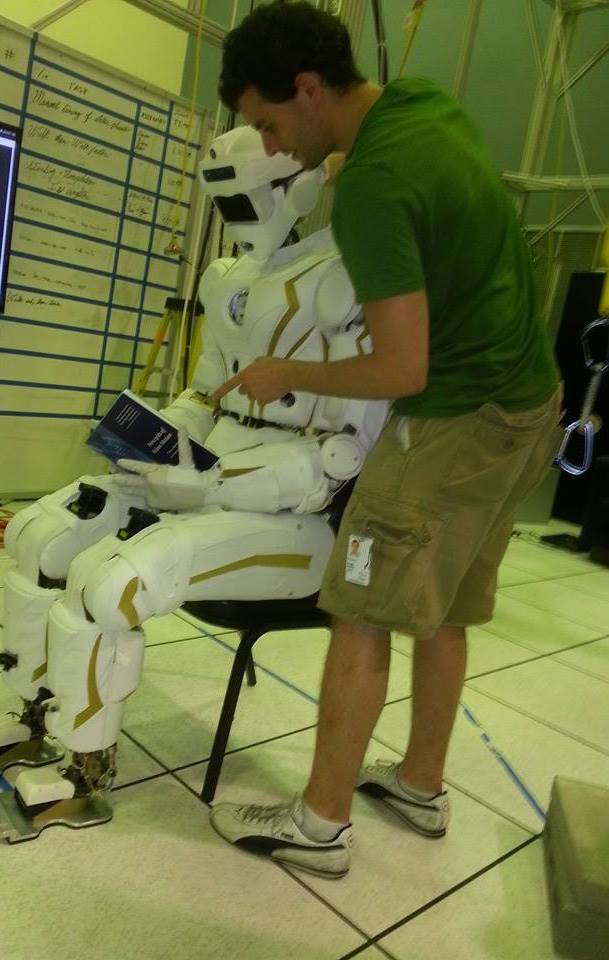
\includegraphics[height=4.0cm]{sinnet_valkyrie}
      \end{figure}
    \end{column}
    \begin{column}{.333\textwidth}
      \begin{figure}
        \centering
        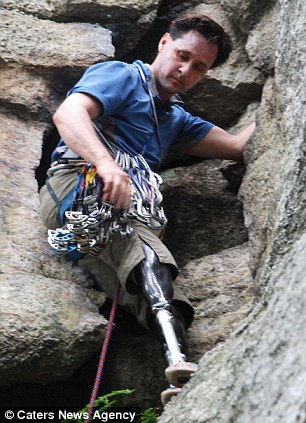
\includegraphics[height=4.0cm]{hugh_herr_climbing}
      \end{figure}
    \end{column}
    \begin{column}{.333\textwidth}
      \begin{figure}
        \centering
        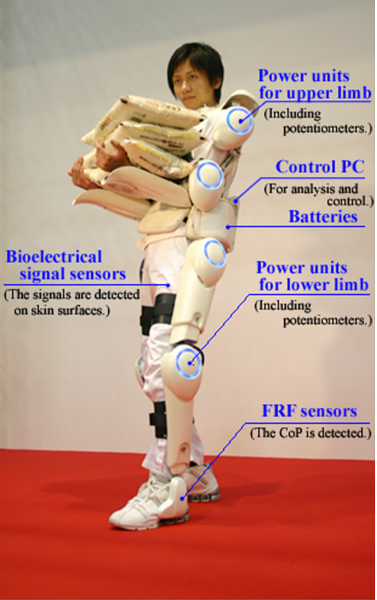
\includegraphics[height=4.0cm]{exoskeleton}
      \end{figure}
    \end{column}
  \end{columns}
\end{frame}

\begin{frame}[t]
  \only<1> {
    {\Large \bf Biomechanics}
    \begin{itemize}
    \item
      D.~A. Winter, {\em Biomechanics and Motor Control of Human Movement}, 2nd ed., New York: Wiley-Interscience, 1990.\\
    \item
      J. Perry and J. Burnfield, Gait Analysis: Normal and Pathological Function, 2nd ed., Thorofare: Slack Inc., 2010.\\
    \end{itemize}
  }
  \only<2,3> {
    \textcolor{gray}{\Large \bf Biomechanics}\\[1mm]
  }

  \only<2> {
    {\Large \bf Reduction-Based Control}
    \begin{itemize}
    \item
      A.~D. Ames et al., {\em On the Geometric Reduction of Controlled Three-Dimensional Bipedal Robotic Walkers}, in 3rd Workshop on Lagrangian and Hamiltonian Methods for Nonlinear Control (LHMNL'06), Nagoya, Japan, Jul. 2006.\\
    \item
      R.~W. Sinnet et al., {\em 3D Bipedal Walking with Knees and Feet: A Hybrid Geometric Approach}, in 48th IEEE Conference on Decision and Control, Shanghai, P. R. China, Dec. 2009.
    \item
      R~.W. Sinnet and A.~D. Ames, {\em Bio-Inspired Feedback Control of Three-Dimensional Humanlike Bipedal Robots}, in Journal of Robotics and Mechatronics, special issue on {\em Focused Areas and Future Trends in Bio-Inspired Robots}, Aug. 2012.

    \end{itemize}
  }
  \only<1,3> {
    \textcolor{gray}{\Large \bf Reduction-Based Control}\\[1mm]
  }

  \only<3> {
    {\Large \bf Human-Inspired Control}
    \begin{itemize}
    \item
      A.~D. Ames, {\em First Steps Toward Automatically Generating Bipedal Robotic Walking from Human Data}, in 8th International Workshop on Robotic Motion and Control, Gron{\'o}w, Poland, Jun. 2011.
    \item
      R.~W. Sinnet et al., {\em A Human-Inspired Hybrid Control Approach to Bipedal Robotic Walking}, in 18th IFAC World Congress (IFAC 2011), Milan, Italy, Sep. 2011.
    \item
      R.~W. Sinnet et al., {\em A Human-Inspired Framework for Bipedal Robotic Walking Design}, International Journal of Biomechatronics and Biomedical Robotics, Jan. 2014.
    \end{itemize}
  }
  \only<1,2> {
    \textcolor{gray}{\Large \bf Human-Inspired Control}
  }

\end{frame}

\begin{frame}[t]
  \frametitle{History}
  \begin{columns}

    \begin{column}{.24\textwidth}
      \textcolor{blue}{Passive Walking:}
      \begin{figure}
        \centering
        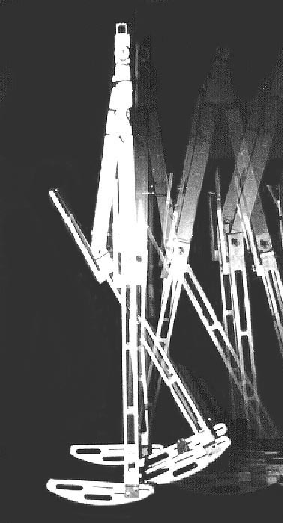
\includegraphics[height=4.5cm]{bipeds_ruina}
      \end{figure}
    \end{column}

    \begin{column}{.24\textwidth}
      \textcolor{blue}{Passivity-Based Control:}
      \begin{figure}
        \centering
        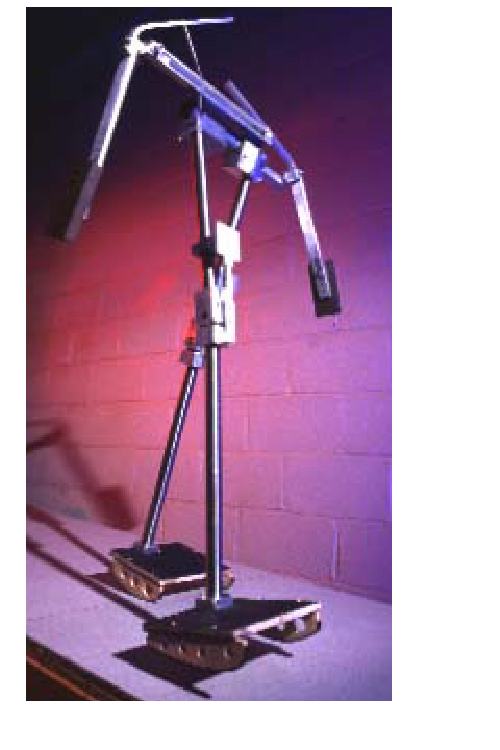
\includegraphics[height=4.5cm]{bipeds_collins}
      \end{figure}
    \end{column}

    \begin{column}{.24\textwidth}
      \textcolor{blue}{Hybrid Zero Dynamics:}
      \begin{figure}
        \centering
        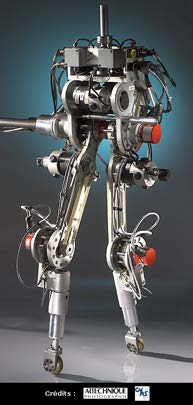
\includegraphics[height=4.5cm]{bipeds_grizzle}
      \end{figure}
    \end{column}

    \begin{column}{.24\textwidth}
      \textcolor{blue}{Human-Inspired Control:}
      \begin{figure}
        \centering
        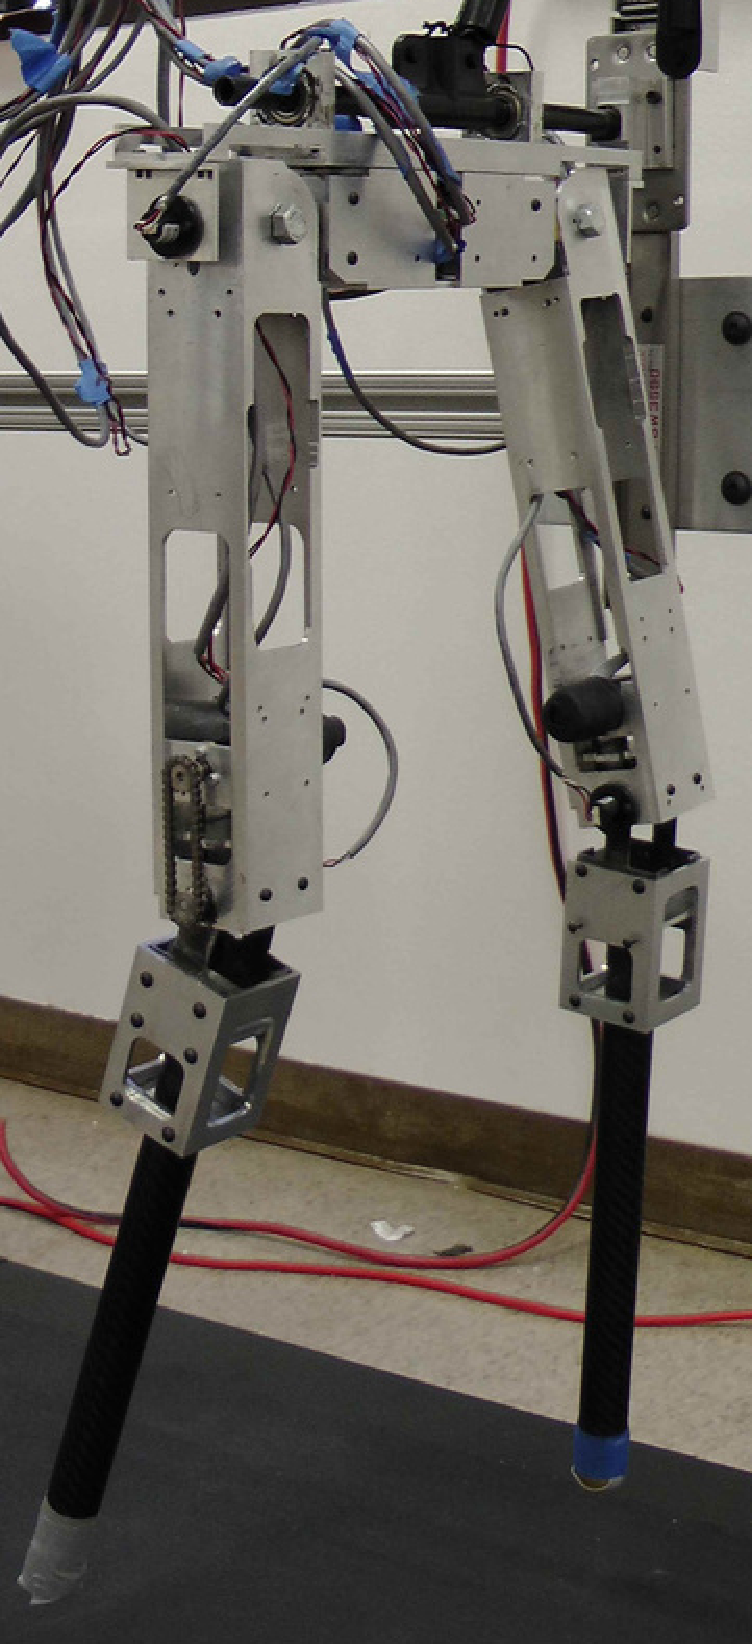
\includegraphics[height=4.5cm]{bipeds_ames}
      \end{figure}
    \end{column}

  \end{columns}
\end{frame}
}{}
\ifdefstring{\PRELIMSECB}{1}{\section{Mechanics}
\showtoc

\subsection{Hybrid Systems}
\begin{frame}[t]
  \frametitle{Bipedal Models}
  \begin{figure}
    \centering
    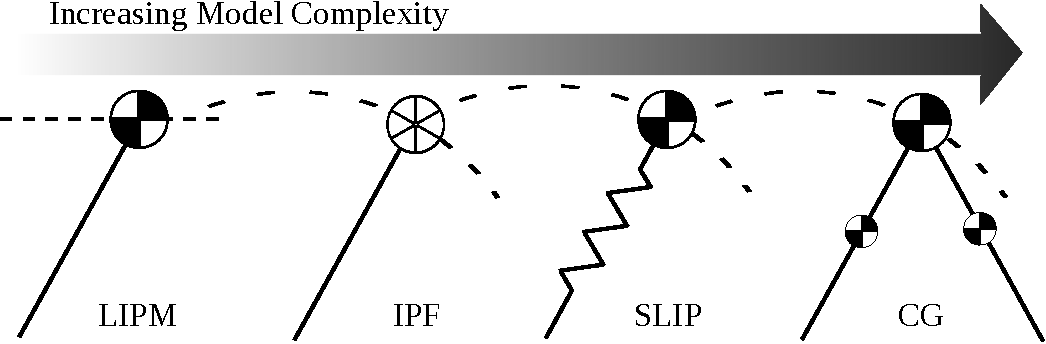
\includegraphics[width=.9\textwidth]{biped-models}
  \end{figure}
  \begin{itemize}
  \item Bipedal locomotion has been studied with a variety of models.
  \item Pendulum models consider massless legs with no impacts.
  \item Kinematic chains are markedly more complex than pendula.
  \end{itemize}
\end{frame}

\begin{frame}[t]
  \frametitle{Modeling Hybrid Systems}
  \begin{columns}
    \begin{column}{.63\textwidth}
      \begin{definition}
        A \alert{hybrid control system} is a tuple \vspace{-.3cm}
        $$\HCS = \hcsystem, \vspace{-.4cm}$$
        where
        \begin{itemize}
        \item
          $\Domain \subset \X$ is the \blue{domain of admissibility} with state space $\X$,
        \item
          $\ControlSet$ is a set of \blue{admissible controls},
        \item
          $\Guard$ is a \blue{guard} or \blue{switching surface},
        \item
          $\ResetMap$ is a smooth \blue{reset map},
        \item
          $(\xf, \xg)$ is a \blue{control system} on $\Domain$: \vspace{-3mm}
          \begin{align*}
            \dx = \xf(\x) + \xg(\x) \, \uu.
          \end{align*}
        \end{itemize}
      \end{definition}
    \end{column}
    \begin{column}{.4\textwidth}
      \begin{figure}    
        \centering
        \def\svgwidth{.8\columnwidth}
        \input{../figs/simple_hybrid_system.eps_latex}
      \end{figure}
      \vspace{-1em}
      A \alert{simple hybrid system}:\vspace{-.5em}
      $$\HS = \hsystem$$
    \end{column}
  \end{columns}
\end{frame}

\begin{frame}[t]
  \frametitle{Lagrangian Systems}
  Mechanical systems are defined by:
  \begin{itemize}
  \item Kinetic energy, $T : T\sQ \to \Rnn$,\\
  \item Potential energy, $U : \sQ \to \R$,
  \end{itemize}
  which together comprise the Lagrangian,
  \begin{align*}
    \Lagrangian\argsqdq = T\argsqdq - U\argsqdq.
  \end{align*}
  Dynamical motion in such a system with external forcing $\mathcal{F} = B\argsq u$ is governed by the Euler--Lagrange equation:
  \begin{align*}
    \frac{d}{dt} \pd{\Lagrangian}{\dq} - \pd{\Lagrangian}{\q} = B\argsq u.
  \end{align*}
\end{frame}

\begin{frame}[t]

  \frametitle{Swing Phase Dynamics}
  \begin{columns}
    \begin{column}{.55\textwidth}
      For Lagrangian $\Lagrangian$ with coordinates
      \begin{align*}
        \x = \argsqdq \in T\ConfigurationSpace,
      \end{align*}
      the dynamic model has the form
      \begin{align*}
        \M\argsq \, \ddq + \C\argsqdq \, \dq + \G\argsq = \B\argsq \, \uu,
      \end{align*}
      or $\dx = \xf\argsqdq+ \xg\argsq \, \uu,$ with
      \begin{align*}
        \xf\argsqdq &= \left(\!\!\begin{array}{c}
            \dq\\
            \M^{-1}\argsq (-\C\argsqdq \, \dq - \G\argsq)
          \end{array}\!\!\right),\\
        \xg(\q) &= \left(\!\!\begin{array}{c}
            \mathbf{0}_{m \times m}\\
            \M^{-1}(\q) \B(\q)
          \end{array}\!\!\right).
      \end{align*}
    \end{column}\!\!
    \begin{column}{.45\textwidth}
      \begin{figure}
        \centering
        \vspace{-10mm}
        \caption{Physical configuration}
        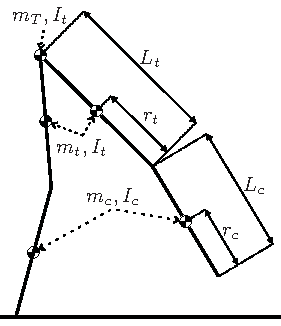
\includegraphics[width = 1.0\columnwidth]{pointfoot_robot_config}
      \end{figure}
    \end{column}
  \end{columns}
\end{frame}

\begin{frame}[t]
  \frametitle{Impact Dynamics}
  Introduce extended coordinates $\qe = (X, \q) \in \mathrm{SE}(3) \times \ConfigurationSpace$ which contains the kinematics of a reference point on the robot. Angular momentum balance based on H{\"u}rm{\"u}zl{\"u} and Marghitu:
  \begin{massump}
    \begin{itemize}
    \item Rigid-body plastic impacts
    \item Enough friction to prevent slipping
    \item Motors do not produce impulses
    \item No instantaneous change in configuration, i.e., $\qe^{-} = \qe^{+}$
    \end{itemize}
  \end{massump}
  Under these assumptions, the discrete dynamics satisfies
  \begin{align*}
    \left[\begin{array}{c c}
        \D_{e}(\qe) & -\Jacobian^{T}(\qe)\\
        \Jacobian(\qe) & \mathbf{0}_{3 \times 3}
      \end{array}\right]
    \left[\begin{array}{c}
        \dq^{+}\\
        \delta F(\qe, \dqe)
      \end{array}\right]
    = \left[\begin{array}{c c}
        \D_{e}(\qe) \, \dqe^{-}\\
        \mathbf{0}_{3}
      \end{array}\right].
  \end{align*}
\end{frame}

\subsection{Solutions to Hybrid Systems}
\begin{frame}[t]
  \frametitle{Hybrid Flows}
  A \alert{hybrid flow} of $\HS$ is a tuple
  \begin{align*}
    \chi^{\HS} = \left( \Delta, \mathscr{I}, \mathscr{C} \right),
  \end{align*}
  \vspace{-2em}
  \begin{itemize}
  \item $\Delta = \{0, 1, 2, \ldots\} \subseteq \Nat$ is a finite or infinite \blue{indexing set},
  \item $\mathscr{I} = \{I_{i} \}_{i \in \Delta}$ is a \blue{hybrid interval} where $I_{i} = [\tau_{i}, \tau_{i + 1}]$,
  \item $\mathscr{C} = \{c_{i} \}_{i \in \Delta}$ is a \blue{collection of solutions} of $\xf$, i.e., ${\dot c}_{i}(t) = \xf(c_{i}(t))$ $\forall i \in \Delta$.
  \end{itemize}

  \only<1>{
    \vspace{-1em}
    \begin{figure}
      \centering
      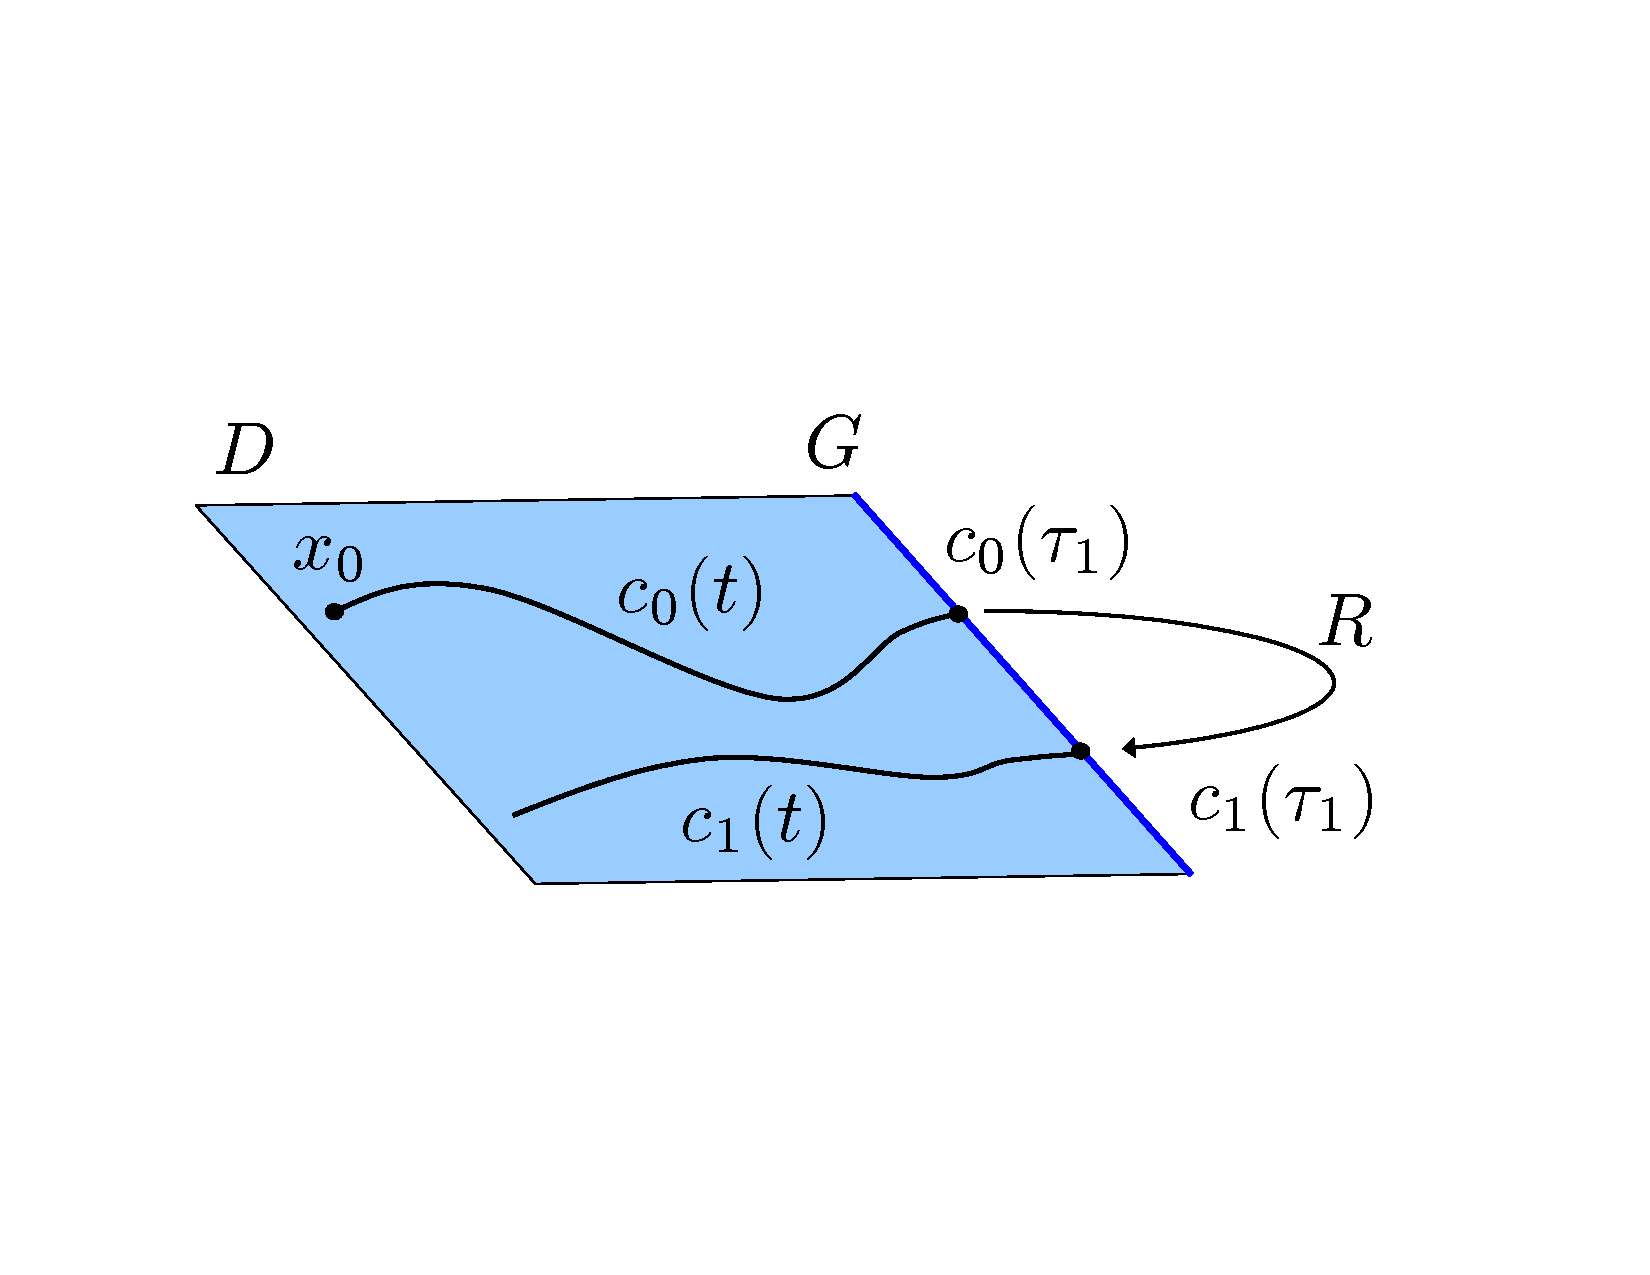
\includegraphics[width=0.5\columnwidth]{hybridflow}
    \end{figure}
    \vspace{-1em}
  }

  \only<2>{
    In addition, for every $i, i + 1 \in \Delta$, it is required that
    \begin{enumerate}
    \item $c_{i}(\tau_{i+1}) \in G$ and
    \item $\Delta(c_{i}(\tau_{i+1})) = c_{i+1}(\tau_{i+1})$
    \end{enumerate}
  }
\end{frame}


\begin{frame}[t]
  \frametitle{Periodic Orbits}
  \begin{figure}    
    \centering
    \def\svgwidth{.45\columnwidth}
    \input{../figs/hybrid_periodic_orbit.eps_latex}
    \caption{A hybrid periodic orbit. Stability is ascertained using the method of Poincar\'e.}
  \end{figure}
\end{frame}

\begin{frame}[t]
  \frametitle{Conservative Systems}
  For a conservative system, total energy is conserved; i.e.:
  \begin{align*}
    \Ec &= T\argsqdq + U\argsq\\
    &= \E(q(0), \dot q(0)) = \E_{0}
  \end{align*}
  Dynamical motion for such a system relies on the interplay between kinetic and potential energy, which is expressed in the Euler-Lagrange equation,
  \begin{align*}
    \frac{d}{dt} \pd{\Lagrangian}{\dq} - \pd{\Lagrangian}{\q} = 0.
  \end{align*}
\end{frame}


\begin{frame}[t]
  \frametitle{The Simplest Example: Passive Compass-Gait Biped}
  \only<1>{
    \begin{columns}
      \column{1.5in}
      Dynamic Model:
      \begin{align*}
        \M\argsq \ddot q + \CG\argsqdq = 0
      \end{align*}
      Control Law:
      \begin{align*}
        \uu = 0.
      \end{align*}
      \column{1.5in}
      \begin{figure}%width=1.0\columnwidth,
        
        \centering
        \def\svgwidth{1.0\columnwidth}
        \input{../figs/cg2d-slope-model.eps_latex}
        \vspace{-2em}
        \caption{Compass-gait biped falling down a slope.}
      \end{figure}
    \end{columns}
  }

  \only<2>{
    \begin{figure}
      \includemedia[
      % width=1.0\columnwidth,
      % height=0.5625\columnwidth,
      %width=1.0\columnwidth,
      %height=0.5\columnwidth,
      width=.9\columnwidth,
      height=0.45\columnwidth,
      addresource=cg2d_slope.mp4,
      activate=pageopen,
      flashvars={source=cg2d_slope.mp4&loop=true&autoPlay=true}
      ]{}{VPlayer9.swf}
      \caption{Stable passive gaits can be found for a range of slopes.}
    \end{figure}    
  }

  \only<3>{
    \begin{figure}
      \centering
      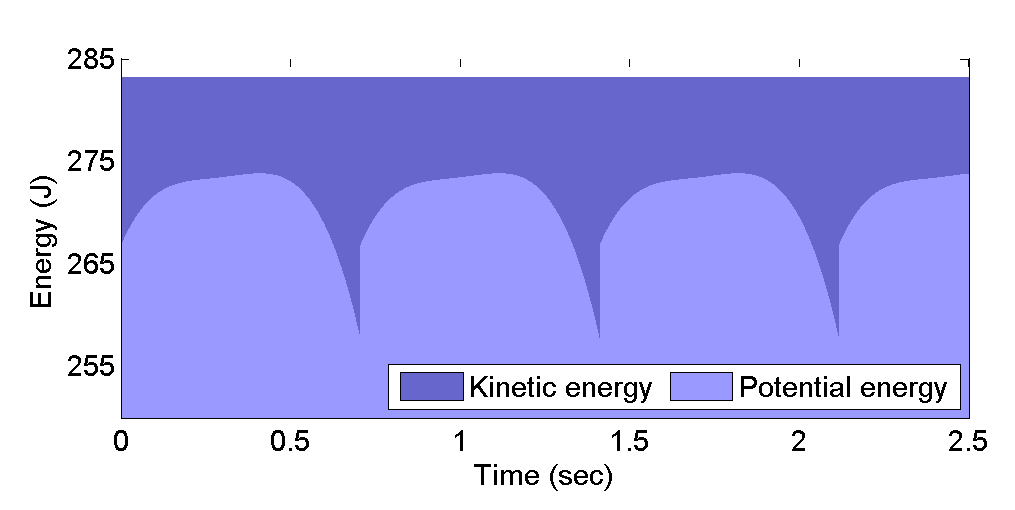
\includegraphics[width=1.0\columnwidth]{energy_cg2d_slope_model}
      \caption{Energy is exchanged between kinetic and potential in form.}
    \end{figure}    
  }
\end{frame}


\begin{frame}[t]
  \frametitle{Nonconservative Systems}
  For a nonconservative system, energy flows out of the system at a rate of $F_{\nc} \cdot dq$. Thus, the following quantity is conserved:
  \begin{align*}
    \Ec &= T\argsqdq + U\argsq - \int_{t_{0}}^{t} \! F_{\nc} \cdot \frac{dq}{d\tau} \ d\tau\\
    &= \E(q(0), \dot q(0)) = \E_{0}
  \end{align*}
  This equation expresses the interplay between kinetic and potential energy and the flow of energy into and out of the system.
\end{frame}


\begin{frame}[t]
  \frametitle{Example: Active Compass-Gait Biped}
  \only<1>{
    \begin{columns}
      \column{1.5in}
      Dynamic Model:
      \begin{align*}
        \M\argsq \ddq + \CG\argsqdq = \B\argsq \uu.
      \end{align*}
      Controlled Symmetries:
      \begin{align*}
        \uu &= \G\argsq - G(\Psi_{\gamma}\argsq)
      \end{align*}
      where $\Psi : \S \times \R \to \sQ$ rotates the frame of gravity by $\gamma$.

      \column{1.5in}
      \begin{figure}
        \centering
        \def\svgwidth{1.0\columnwidth}
        \input{../figs/cg2d-2link-model.eps_latex}
        \vspace{-2em}
        \caption{Compass-gait biped with Controlled Symmetries.}
      \end{figure}
    \end{columns}
  }
  \only<2>{
    \begin{figure}
      \includemedia[
      % width=1.0\columnwidth,
      % height=0.5625\columnwidth,
      width=.9\columnwidth,
      height=0.45\columnwidth,
      addresource=cg2d_2link_simulation.mp4,
      activate=pageopen,
      flashvars={source=cg2d_2link_simulation.mp4&loop=true&autoPlay=true}
      ]{}{VPlayer9.swf}
      \caption{Passive downhill gaits can be translated to flat ground with Controlled Symmetries.}
    \end{figure}    
  }
  \only<3>{
    \begin{figure}
      \centering
      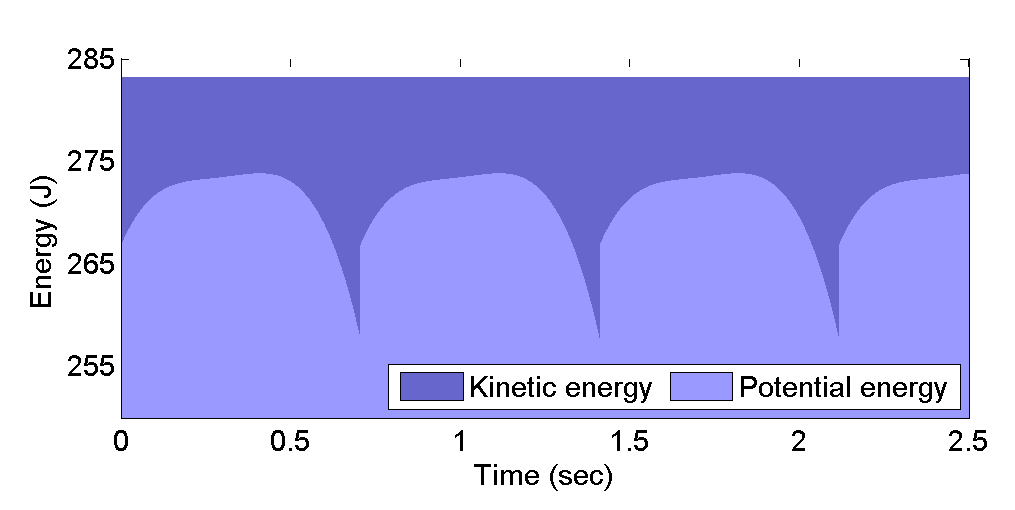
\includegraphics[width=1.0\columnwidth]{energy_cg2d_slope_model}
      \caption{Energy of the shaped system is conserved.}
    \end{figure}    
  }
\end{frame}

\begin{frame}[t]
  \frametitle{Example: 3-Link Biped}
  \only<1>{
    \begin{columns}
      \column{1.5in}
      Dynamic Model:
      \begin{align*}
        \M\argsq \ddq + \CG\argsqdq = \B\argsq \uu
      \end{align*}
      Control Law:
      \begin{align*}
        \uu &= \G\argsq - \G(\Psi\argsq)\\
        \uu_3 &=-k_{d} (\dot \vartheta_{T}^{a})\\
        &\hspace{1.8em} -k_{p} (\vartheta_{T}^{a} - \vartheta_{T}^{d})
      \end{align*}
      \column{1.5in}
      \begin{figure}
        \centering
        \def\svgwidth{1.0\columnwidth}
        \input{../figs/cg2d-3link-model.eps_latex}
        \vspace{-2em}
        \caption{3-link biped configuration.}
      \end{figure}
    \end{columns}
  }

  \only<2>{
    \begin{figure}
      \centering
      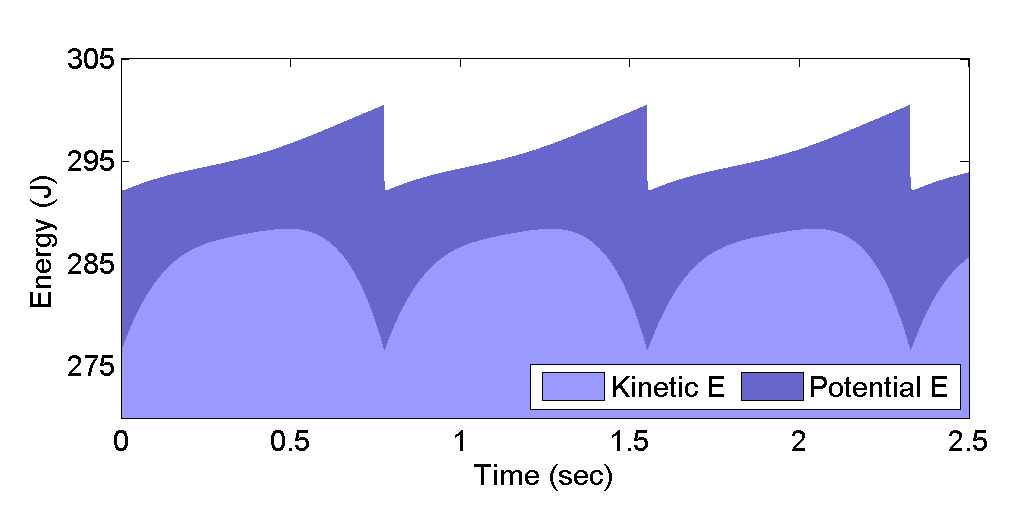
\includegraphics[width=1.0\columnwidth]{energy_cg2d_3link}
      \caption{Energy is not conserved as the controller injects energy.}
    \end{figure}
  }

  \only<3>{
    \begin{figure}
      \includemedia[
      %width=1.0\columnwidth,
      %height=0.5\columnwidth,
      width=.9\columnwidth,
      height=0.45\columnwidth,
      addresource=cg2d_3link_simulation.mp4,
      activate=pageopen,
      flashvars={source=cg2d_3link_simulation.mp4&loop=true&autoPlay=true}
      ]{}{VPlayer9.swf}
      \caption{Stable passive gaits can be found for a range of slopes.}
    \end{figure}
  }
\end{frame}
}{}
\ifdefstring{\PRELIMSECC}{1}{\section{Energy Shaping}
\showtoc

\subsection{Energy Shaping with Control Lyapunov Functions}

\begin{frame}[t]
  \frametitle{Motivation}
  \begin{block}{Main Question}
    Can we use an understanding of energy exchange to improve robustness  of
    periodic orbits in hybrid mechanical systems?
  \end{block}

  \begin{block}{Observations}
    \begin{itemize}
    \item Numerous control design schemes exist for stabilizing hybrid mechanical
      systems to periodic orbits.
    \item Some controllers produce good behavior locally but lack robustness.
    \item Periodic orbits have associated energy functions with level sets which
      are invariant under the orbits.
    \end{itemize}
  \end{block}
\end{frame}

\begin{frame}[t]
  \frametitle{Overview}
  \begin{block}{Main Idea}
    Add robustness to a periodic behavior by imposing convergence on a conserved
    energy function, $\Ec : \x \to \R$, to a level set which is known to be
    invariant under the system dynamics.
  \end{block}
  
  \begin{block}{Control Objective}
    Choose control input $\mu\arx$ such that $\| \mu\arx \|$ is minimized and
    $\Ec\arxt \to \Eref$ as $t \to \infty$.
  \end{block}

  \begin{block}{Exponential Convergence}
    To achieve exponential stabilization, $\Ec\arxt$ should satisfy\vspace{-.4em}
    \begin{align*}
      \Ec\arxt \leq \Ec\arxzero e^{-\beta t} \mbox{ for } t \geq 0, \beta > 0.
    \end{align*}
  \end{block}
\end{frame}

\begin{frame}[t]
  \frametitle{Conserved Energy Functions}
  \only<1> {
    \begin{block}{Conservative Systems}
      A conservative system with state space $\x = \argsqdq$ is modeled as
      \begin{align*}
        \HCSbar = \left\{
          \begin{array}{l l}
            \left.\begin{array}{r c l}
                \hspace{.58em}\dx &=& \xfbar\argsqdq + \xgbar\argsq \, \uu
              \end{array}\right\}  & \mbox{if } \argsqdq \in \D \setminus \S,\\
            \left. \begin{array}{r c l}
                \qp &=& \Deltaq\argsqm\\
                \dqp &=& \Deltadq\argsqdqm
              \end{array} \right\} & \mbox{if } \argsqdq \in \S,
          \end{array}\right.
      \end{align*}
      where $\xfbar\argsqdq := \xf\argsqdq$ and $\xgbar\argsq := \xg\argsq$ for
      notational clarity. Total energy is conserved through the continuous
      dynamics, i.e.,
      \begin{align*}
        \Ec\argsqdq := T\argsqdq + U\argsq.
      \end{align*}
    \end{block}
  }

  \only<2> {
    \begin{block}{Nonconservative Systems}
      To properly handle the flow of energy due to $\vv\argsqdq$, define a storage
      function, $\W$, which obeys the differential equation
      \begin{align*}
        d\W = \vfR\argsqdq \, dt = \left( \B\argsq \, \vv\argsqdq \right)^{T}
        \frac{d\q}{dt}\art \, dt.
      \end{align*}
      Using $\W$, augment the state space, i.e., $\x := (\q, \dq, \W)$, and the vector
      fields (subsuming $\vv\argsqdq$ under $\xfbar\argsqdq$), i.e, 
      \begin{align*}
        \xfbar\argsqdq := \left(\begin{array}{c}
            \xf\argsqdq + \xg\argsq \, \vv\argsqdq\\
            \vfR\argsqdq
          \end{array}\right), &&
        \xgbar\argsq := \left(\begin{array}{c}
            \xg\argsq\\
            \boldzero
          \end{array}\right).
      \end{align*}
    \end{block}
  }
  \only<3> {
    \begin{block}{Nonconservative Systems}
      Use the augmented state to define the hybrid control system
      \begin{align*}
        \HCSbar = \left\{
          \begin{array}{l l}
            \left.\begin{array}{r c l}
                \hspace{1.15em}\dx &=& \xfbar\argsqdq + \xgbar\argsq \, \uu
              \end{array}\right\}  & \mbox{if } \argsqdq \in \D \setminus \S,\\
            \left. \begin{array}{r c l}
                \qp &=& \Deltaq\argsqm\\
                \dqp &=& \Deltadq\argsqdqm\\
                \Wp &=& \DeltaW = 0
              \end{array} \right\} & \mbox{if } \argsqdq \in \S.
          \end{array}\right.
      \end{align*}
      For such a system, the following quantity is conserved:
      \begin{align*}
        \Ec\argsqdqW := T\argsqdq + U\argsq - W.
      \end{align*}
    \end{block}
  }
\end{frame}

\begin{frame}[t]
  \frametitle{Rapidly Exponentially Stabilizing CLFs}
  A \blue{rapidly exponentially stability control Lyapunov function (RES--CLF)}
  $\Ve : \X \to \Rnn$ satisfies
  \begin{align*}
    &c_{1} \nx^{2} \leq \Ve\arx \leq \frac{c_{2}}{\resclfparam^{2}} \nx^{2},\\
    &\inf_{\uu \in \U} \Lie{\xfbar}\Ve\arx + \Lie{\xgbar}\Ve\arx \, \uu +
    \frac{c_{3}}{\resclfparam} \Ve\arx \leq 0
  \end{align*}
  for $c_{1}, c_{2}, c_{3} > 0$ exhibits exponential convergence. If the above
  are satisfied, then it is also true that
  \begin{align*}
    \left\| \pd{\Ve\arx}{\x} \right\| \leq c_{4} \nx.
  \end{align*}
\end{frame}

\begin{frame}[t]
  \frametitle{Energy Shaping}
  Consider a conserved energy function $\Ec\arx$ on a hybrid control system
  $\HCSbar$ which has a periodic orbit $\orbit$ and define a Lyapunov candidate:
  \begin{align*}
    V\arx = \frac{1}{2} \left(\Ec\arx - \Eref\right)^{2},
  \end{align*}
  with $\Eref$ the constant energy level of the system on the orbit
  $\orbit$. For a RES--CLF, we seek a feedback control law, $\mu\arx$, such that
  \begin{align*}
    \Lie{\xfbar} V\arx + \Lie{\xgbar} \V\arx \, \mu\arx + \epsilon \V\arx &\leq 0.
  \end{align*}
\end{frame}

\begin{frame}[t]
  \frametitle{Quadratic Program Formulation}
  The linear form of the RES--CLF condition suggests
  \begin{align}
    \nonumber
    \mueps\arx = \argmin_{\uu \in \R^{n}}  \, & \uu^T \uu,\\
    \mbox{s.t. } & \Aclf\arx \, \uu \leq \bclf\arx
  \end{align}
  which encodes the dynamics of the system. This controller imposes exponential
  stabilization of the energy as defined by the RES--CLF.
\end{frame}

\begin{frame}[t]
  \frametitle{Main Theorem}
  \begin{block}{Theorem [Energy Shaping]}
    Given an exponentially-stable cycle in a hybrid system, application
    of the energy shaping controller results in the closed-loop hybrid system
    \begin{align*}
      \HS_{\resclfparam} = \left\{
        \begin{array}{r c l l}
          \dx &=& \xfbar\arx + \xgbar\arx \, \mueps\arx, & \x \in \D \setminus \S,\\
          \xp &=& \Delta(\xm), & \x \in \S,
        \end{array}\right.
    \end{align*}
    which is exponentially stable about the hybrid periodic orbit $\orbit$ for
    large enough $\resclfparam$.
  \end{block}
\end{frame}

\subsection{Sketch of Proof}

\begin{frame}[t]
  \frametitle{Overview of Proof}
  \begin{block}{Sketch of Proof [Energy Shaping]}
    \begin{enumerate}
    \item Transform the coordinates into a more intuitive form.
    \item Define a discrete Lyapunov candidate function valid on the \Poincare{} map.
    \item Show the conditions for stability through bounding arguments.
    \end{enumerate}
  \end{block}
\end{frame}

\begin{frame}[t]
  \frametitle{Zero Dynamics Formulation}
  Construct a change of coordinates, splitting up the system into two sets of
  coordinates:
  \begin{align*}
    \dot \zdx &= f\argsxz + g\argsxz \, \uu,\\
    \dot \zdz &= q\argsxz + w\argsxz \, \uu.
  \end{align*}
  The vector fields $f$, $g$, $q$, and $w$ are assumed to be locally Lipschitz
  continuous. For simplicity, define
  \begin{align*}
    \bigF\argsxz = \left(\begin{array}{c}
        f\argsxz\\
        q\argsxz
      \end{array}\right),&&
    \bigG \argsxz = \left(\begin{array}{c}
        g\argsxz\\
        w\argsxz
      \end{array}\right).
  \end{align*}
\end{frame}

\begin{frame}[t]
  \frametitle{Energy-Based Coordinate Change}
  \only<1> {
    \begin{block}{Conservative Systems}
      Using the state $\x = \argsqdq$, construct the transformation
      $\xform\argsqdqW := \argsxz$ where
      \begin{align*}
        \zdx &= \Ec\argsqdq - \Eref,\\
        \zdz &= \xrem,
      \end{align*}
    \end{block}
  }

  \only<2> {
    \begin{block}{Nonconservative Systems}
      Using the state $\x = \argsqdqW$, construct the transformation
      $\xform\argsqdqW := \argsxz$ where
      \begin{align*}
        \zdx &= \Ec\argsqdqW - \Eref,\\
        \zdz &= \xremW,
      \end{align*}
    \end{block}
  }
  where $n$ is the size of the configuration space, $\Q$. The fixed point of the
  hybrid system is chosen to occur at $\argsxz = \xzst$ such that $\Delta\xzst =
  \argszero$.
\end{frame}

\begin{frame}[t]
  \frametitle{Validity of Transformation}
  \only<1> {
    \begin{block}{Conservative Systems}
      The coordinate change $\xform\arx = \xform\argsqdq$ is valid if it is locally
      diffeomorphic around the orbit $\orbit$, i.e., if
      \begin{align*}
        \pd{\xform\argsqdq}{\argsqdq} =
        \left(\begin{array}{c c}
            I_{2n-1} & \boldzero_{2n-1 \times 1}\\
            \pd{\Ec(\q, \dq)}{\xrem} & \pd{\Ec(\q, \dq)}{\dq_{n}}
          \end{array}\right)
      \end{align*}
      % 
      has full rank, which occurs when
      \begin{align*}
        \det\left(\pd{\xform\argsqdq}{\argsqdq}\right) =
        \pd{\Ec\argsqdq}{\dq_{n}} \ne 0.
      \end{align*}
    \end{block}
  }
  
  \only<2> {
    \begin{block}{Nonconservative Systems}
      The coordinate change $\xform\arx = \xform\argsqdqW$ is valid if it is
      locally diffeomorphic around the orbit $\orbit$, i.e., if
      \begin{align*}
        \pd{\xform\argsqdqW}{\argsqdqW} =
        \left(\begin{array}{c c c}
            I_{2n-1} & \boldzero_{2n-1 \times 1} & \boldzero_{2n-1 \times 1}\\
            \pd{\E\argsqdqW}{\xrem} & \pd{\Ec\argsqdqW}{\dq_{n}} & 1\\
            \boldzero_{1 \times 2n-1} & 0 & 1
          \end{array}\right)
      \end{align*}
      % 
      has full rank, which occurs when
      \begin{align*}
        \det \pd{\xform\argsqdqW}{\argsqdqW} = \pd{\Ec\argsqdqW}{\dq_{n}} \ne 0.
      \end{align*}
    \end{block}
  }
\end{frame}

\begin{frame}[t]
  \frametitle{Flows of Continuous Dynamical Systems}
  The flow of an ODE expressed in the variables $\argsxz$ is given
  by
  \begin{align*}
    \flowt\argsxz = \int_{0}^{t} \left[ \bigF\argsxztau + \bigG\argsxztau \,
      \uu\argsxztau \right] \, d\tau
  \end{align*}
  for some feedback control law $\uu : \zdX \times \zdZ \to \U$. For some stable
  tube $\stabletube$ around the orbit $\orbit$, it holds that the vector fields
  are bounded:
  \begin{align*}
    \supF & := \sup \left\{ \left\| \bigF\argsxz \right\| : \argsxz \in
      \stabletube \right\},\\
    \lambdamaxG &:= \sup \left\{\lambdamax\bigG\argsxz : \argsxz \in \stabletube
    \right\},\\
    \lambdaminG &:= \inf \left\{\lambdamin\bigG\argsxz : \argsxz \in \stabletube
    \right\}.
  \end{align*}
\end{frame}


\begin{frame}[t]
  \frametitle{Definition of the \Poincare{} Map}
  \only<1> {
    The \blue{\Poincare{} first return map} takes a point on the guard, applies
    the reset map and then integrates forward until the guard is reached
    again. For the shaped system, $\Pe : \S \to \S$, is defined by
    \begin{align*}
      \Pe\argsxz = \floweps_{\TIeDelta}\argsDeltaxz,
    \end{align*}
    where $\TIe : \zdX \times \zdZ \to \Rnn$ is the \tti{} function which is
    defined by
    \begin{align*}
      \TIe\argsxz = \inf \{ t \geq 0 : h(\flowepst\argsxz) \}
    \end{align*}
    and is locally Lipschitz continuous by the implicit function theorem.
  }

  \only<2> {
    \begin{figure}    
      \centering
      \def\svgwidth{.78\columnwidth}
      \input{../figs/poincare_return_map.eps_latex}
      \caption{The \Poincare{} map is defined by the \tti{} function and maps
        from states on the \Poincare{} section $\S$ back to the section.}
    \end{figure}
  }

  \only<3> {
    Using the change of coordinates $\rho(\resclfparam) :=
    \tfrac{1}{\resclfparam}$, define the function
    \begin{align*}
      N(t, \rho, \zdx, \zdz) = h(\flowrhot(\Deltaxz)),
    \end{align*}
    By the implicit function theorem, there exists a $\delta > 0$ and a unique
    function $\taurho(\rho, \zdx, \zdz)$ defined and locally Lipschitz for all
    $(\rho, \zdx, \zdz) \in \B_{\delta}(0, 0, \zdzst)$ such that $\tau^{0}(0,
    \zdzst) = \TI(0, \zdzst) = \Tst$ where $\Tst$ is the period of the invariant
    orbit $\orbit$.\\ \ \\

    Selecting a fixed $\resclfparam > 0$ with the min-norm controller, it
    follows that for some $\delta > 0$ and $\argsxz \in \B_{\delta}\xzst \cap
    \S$,
    \begin{align*}
      \label{eq:TIe-bounds}
      0.9 \Tst \leq \TIe\argsxz \leq 1.1 \Tst.
    \end{align*}
  }
\end{frame}

\begin{frame}[t]
  \frametitle{Equivalence of Hybrid Periodic Orbits}
  \begin{lemma}[Equivalence of Orbits]
    Applying the energy shaping controller to the hybrid control system $\HCSbar$
    results in the closed-loop hybrid system $\HSepsbar$ that demonstrates a
    periodic orbit which is identical to the unshaped system $\HSbar$.
  \end{lemma}
  \begin{block}{Proof}
    The energy of states $\xo \in \orbit$ is a constant,
    $\E(\xo) \equiv \Eref$. By the choice of Lyapunov function,
    $\V(\xo) \equiv 0$. In addition, $\dV(\xo) \equiv 0$ since
    the system is conservative. And since the solution to the optimization
    problem has cost $\uu^{T}(\xo) \uu(\xo) \equiv 0$, the
    control effort is also zero. Hence the orbits are equivalent.
  \end{block}
\end{frame}

\begin{frame}[t]
  \frametitle{Boundedness of \TtI{} Function}
  \only<1> {
    The difference in solutions between the shaped and unshaped systems can be
    bounded by examining the difference in solutions:
    \begin{lemma}[Boundedness of \TtI{}]
      For the hybrid systems $\HSbar$ and $\HSepsbar$,
      \begin{eqnarray}
        \nonumber
        &| \TIe(\Deltaxz) - \TI(\Deltaxz) | \leq \ATIe \nzdxzst,
      \end{eqnarray}
      where $\limeps \ATIe = 0$.
    \end{lemma}
  }
  
  \only<2> {
    \begin{block}{Proof (Boundedness of \TtI{})}
      Construct an auxiliary \tti{} function $\TB$ which is locally Lipschitz
      continuous and independent of $\resclfparam$:
      \begin{align*}
        \TB(\eta, \zdx, \zdz) = \inf\{t \geq 0 : h(\eta + \flowt(\Delta(0,
        \zdzst))) = 0\}.
      \end{align*}
      By construction,
      \begin{align*}
        \TB(0, \zdx, \zdz) = \TI\argsxz.
      \end{align*}
    \end{block}
  }

  \only<3> {
    \begin{block}{Proof (Boundedness of \TtI{})}
      Let $\argsxzti{1}$ and $\argsxzti{2}$ satisfy\vspace{-.4em}
      \begin{align*}
        \argsDxzti{1} = \floweps\argsxzti{1}, && \argsDxzti{2} =
        \flow\argsxzti{2},
      \end{align*}
      with initial conditions $\argsxzizero{1} = \argsxzizero{2} = \Delta(0,
      \zdzst)$. Define
      \begin{align*}
        \etaeps = \left.\argsxzti{1}\right|_{t = \TIe\argsxz} -
        \left.\argsxzti{2}\right|_{t = \TIe\argsxz}
      \end{align*}
      and as a result,\vspace{-.4em}
      \begin{align*}
        \TIe\argsxz = \TB(\etaeps, \zdx, \zdz).
      \end{align*}
    \end{block}
  }

  \only<4> {
    \begin{block}{Proof (Boundedness of \TtI{})}
      Examining the explicit solution given by the min-norm control law,
      \begin{align*}
        \mueps\argsxz = - \frac{\frac{c_{3}}{\resclfparam} \Ve\argsxz
          \bigG^{T}\argsxz \left( \pd{V_{e}\argsxz}{\argsxz}
          \right)^{T}}{\pd{V_{e}\argsxz}{\argsxz} \bigG\argsxz \bigG^{T}\argsxz
          \left( \pd{V_{e}\argsxz}{\argsxz} \right)^{T}},
      \end{align*}
      a bound can be established:
      \begin{align*}
        \| \mueps\argsxz \| \leq \frac{c_{2}c_{3}}{\resclfparam^{3}} \frac{\lambdamaxG}{\lambdaminG} \nzdx.
      \end{align*}
    \end{block}
  }

  \only<5> {
    \begin{block}{Proof (Boundedness of \TtI{})}
      The difference between flows can then be bounded:
      \begin{align*}
        \|\etaeps\| &\leq \int_{0}^{\TIe\argsxz} \! \left\| \bigG\argsxztau \,
          \mueps\argsxztau \, \right\| d\tau\\
        &\leq \LDelta \frac{c_{2}^{\frac{3}{2}}
          c_{3}^{2}}{2c_{1}^{\frac{1}{2}}\resclfparam^{5}}
        \frac{\lambdamaxG^{2}}{\lambdaminG^{2}}  \, \left(1 -
          e^{-\frac{c_{3}}{2\resclfparam} 1.1 \Tst}\right) \nzdxzst.
      \end{align*}
    \end{block}
  }
  
  \only<6> {
    \begin{block}{Proof (Boundedness of \TtI{})}
      Because $\TB$ is Lipschitz continuous, it follows that
      \begin{align*}
        | \TIe\argsxz - \TI\argsxz | &= | \TB(\etaeps, \zdx, \zdz) - \TB(0,
        \zdx, \zdz)|\\
        &\leq \LB \| \etaeps \|.
      \end{align*}
      Using the bound for $\etaeps$ leads to the conclusion that
      \begin{align*}
        | \TIe(\Deltaxz) - \TI(\Deltaxz) | \leq \ATIe \nzdxzst
      \end{align*}
      with $\limeps \ATIe = 0$. \hfill \qedsymbol
    \end{block}
  }
\end{frame}

\begin{frame}[t]
  \frametitle{Boundedness of \Poincare{} Maps}
  \only<1> {
    The difference in \Poincare{} maps of the unshaped and shaped systems can be
    bounded by examining the difference in solutions:
    \begin{lemma}[Boundedness of \Poincare{} Maps]
      For the hybrid systems $\HSbar$ and $\HSepsbar$,
      \begin{eqnarray}
        \nonumber
        &\| \Pe\argsxz - \P\argsxz \| \leq \Ae \nzdxzst,
      \end{eqnarray}
      where  $\limeps\Ae = 0$.
    \end{lemma}
  }

  \only<2> {
    \begin{block}{Proof (Boundedness of \Poincare{} Maps)}
      By the definition of the \Poincare{} map,
      \begin{align*}
        \lefteqn{\left\| \Pe\argsxz - \P\argsxz \right\| \leq}\\
        & \hspace{2em} \int_{\TIDelta}^{\TIeDelta} \hspace{-2.5em} \left\|
          \bigF\argsxztau \right\| \, d\tau\\
        & \hspace{4em} \mbox{} + \int_{0}^{\TIeDelta} \hspace{-2.5em} \left\|
          \bigG\argsxztau \, \mueps\argsxztau \, \right\| d\tau.
      \end{align*}
    \end{block}
  }

  \only<3> {
    \begin{block}{Proof (Boundedness of \Poincare{} Maps)}
      Using the explicit solution given by the min-norm controller and the bounds
      established on the difference in \tti{} functions, the bounds can be
      evaluated and the result is a bound of the form
      \begin{align*}
        \left\| \Pe\argsxz - \P\argsxz \right\| \leq \Ae \! \nzdxzst,
      \end{align*}
      where  $\limeps\Ae = 0$. \hfill \qedsymbol
    \end{block}
  }
\end{frame}

\begin{frame}[t]
  \frametitle{Proof of Energy Shaping Theorem}
  \only<1> {
    Define a composite Lyapunov function,
    \begin{align*}
      \VP\argsxz = \Vn\argsxz + \sigma \Vex(\zdx),
    \end{align*}
    where
    \begin{itemize}
    \item $\Vn$ : Lyapunov function guaranteed by stability of the nominal system
      (converse Lyapunov theorem)
    \item $\Vex$ : Lyapunov function for energy shaping control law
    \end{itemize}
    with scaling parameter $\sigma$. This is a discrete Lyapunov function that
    is valid on the guard.
  }
  
  \only<2> {
    Exponential stability of the hybrid system $\HS$ is guaranteed by the
    discrete Lyapunov theorem if
    \begin{eqnarray*}
      &r_{1} \nzdxzst^{2} \leq \VP\argsxz \leq r_{2} \nzdxzst^{2}\\
      &\VP(\Pe\argsxz) - \VP\argsxz \leq r_{3} \nzdxzst^{2}
    \end{eqnarray*}
    for some $r_{1}, r_{2}, r_{3} \in \Rnn$.
  }
\end{frame}
}{}
\ifdefstring{\PRELIMSECD}{1}{\section{Geometric Reduction}
\showtoc

\begin{frame}
  \frametitle{Overview}
  diagram
\end{frame}

\subsection{Functional Routhian Reduction}
\begin{frame}
  \frametitle{History}
  \begin{description}[D]
  \item[ Geometric reduction\footnote{For more on geometric reduction, see [Marsden, Springer-Verlag 1994]}:] \hspace{5cm}

    \begin{itemize}
    \item Begin with a Lagrangian $\Lagrangian : T\ConfigurationSpace \to \R$.
    \item Symmetries in the system are characterized by \textcolor{blue}{cyclic}
      variables: $\frac{\partial \Lagrangian}{\partial \phi} = 0$.
    \item The dimensionality of the phase space can be reduced (by ``dividing'' out by the symmetries).
    \item A corresponding Lagrangian, the \textcolor{blue}{Routhian}, can be defined on this reduced phase space.
    \end{itemize}
  \end{description}

  \begin{block}{Geometric Reduction ``Theorem''}
    One can understand the behavior of the full-order system in terms of
    the behavior of the reduced system and vice versa.
  \end{block}
\end{frame}

\begin{frame}
  \frametitle{Motivation}
  \begin{description}[D]
  \item[ Classical Reduction:]  The conserved quantities used to reduce and reconstruct systems are constants.
  \item[ Yet:]  It may be desirable to \alert{vary} the cyclic variables while not affecting the reduced order system.
  \item[ Motivates:]  An extension of Routhian reduction, termed \alert{functional Routhian reduction}, where the conserved quantities are functions of the cyclic variables:
    \begin{itemize}
    \item Allows us to control the cyclic variables.
    \item Can be effectively used to reduce bipedal robotic walkers.
    \item Generalizes to hybrid systems.
    \end{itemize}
  \end{description}
\end{frame}

\begin{frame}
  \frametitle{Almost-Cyclic Lagrangians \& Functional Routhians}
  \vspace{-1mm}

  Consider the case when $\ConfigurationSpace = S \times \S$ where $S$ is called the \textcolor{blue}{shape space}; we denote an element $q \in \ConfigurationSpace$ by $q = (\theta^T, \varphi)^T$.

  \vspace{-1mm}

  \begin{definition}
    A Lagrangian $\Llambda : TS \times T\S \to \R$ is \alert{almost-cyclic} if:
    \vspace{-3mm}
    \begin{align*}
      \Llambda(\theta, \phi, \dot \theta, \dot \phi)  =
      \frac{1}{2} \left(\!\!\begin{array}{cc}
      \dot \theta^T  &  \dot \phi
      \end{array}\!\!\right) \Mlambda(\theta)
      \left(\begin{array}{c}
        \dot \theta\\
        \dot \phi
      \end{array}\right) - \Wlambda(\theta, \phi, \dot \theta) - \Vlambda(\theta, \phi),
    \end{align*}
    for some function $\lambda : \S \to \R$.
  \end{definition}

  \only<1>{
    \vspace{-7mm}
    \textcolor{darkgray}{
      \begin{align*}
        \Mlambda(\theta) &= \left(\begin{array}{cc}
          \textcolor{lightblue}{\Mtheta(\theta)} + \Mphitheta^T(\theta) \Mphi^{-1}(\theta) \Mphitheta(\theta) & \Mphitheta^T(\theta)\\
          \Mphitheta(\theta) \qquad & \Mphi(\theta)
        \end{array}\right),\\[0mm]
        \Wlambda(\theta,\phi,\dot \theta) &= \textcolor{berkeleygold}{\lambda(\varphi)} \Mphi^{-1}(\theta) \Mphitheta(\theta) \dot{\theta},\\[0mm]
        \Vlambda(\theta,\phi) &= \textcolor{lightblue}{\Vt(\theta)} - \frac{1}{2} \textcolor{berkeleygold}{\lambda(\varphi)} \Mphi^{-1}(\theta) \textcolor{berkeleygold}{\lambda(\varphi)}.
      \end{align*}
    }
  }

  \only<2>{
    \begin{definition}
      The corresponding \alert{ functional Routhian} $\Lt : TS \to \R$ is: \vspace{-.3cm}
      \begin{eqnarray*}
        \Lt(\theta, \dot \theta) &=& \left[ \Llambda(\theta, \varphi, \dot{\theta}, \dot{\varphi}) - \lambda(\varphi) \dot{\varphi} \right]_{\Jfcn = \lambda(\varphi)}\\[0mm]
        & = &  \frac{1}{2} \dot{\theta}^T M_\theta(\theta) \dot{\theta} - \Vt(\theta).
      \end{eqnarray*}
    \end{definition}
  }
\end{frame}

\begin{frame}
  \frametitle{Functional Routhian Reduction}

  \begin{theorem}
    {\small Let $\Llambda$ be an almost-cyclic Lagrangian with an almost-cyclic variable, $\varphi$, and $\Lt$ the corresponding functional Routhian with shape space $S = \R^{n - 1}$. Let $\Upsilon : TS \times \S \to \R^n$ represent external forces satisfying:
      \begin{enumerate}
      \item $\Fextt$ does not depend on $\varphi,\dot{\varphi}$,
      \item $\Upsilon_i(\theta,\dot{\theta}) = 0$ for $i = 2, \ldots, n$.
      \end{enumerate}
      Then $(\theta(t), \varphi(t), \dot{\theta}(t), \dot{\varphi}(t))$ is a solution to the forced vector field $f_{\Llambda}$ on $[t_0, t_F]$ with \vspace{-2mm}
      \begin{align*}
        \dot{\varphi}(t_0) = \Mphi^{-1}(\theta(t_0)) (\lambda(\varphi(t_0)) - \Mphitheta(\theta(t_0))\dot{\theta}(t_0)),\\[-7mm]
      \end{align*}
      if and only if $(\theta(t), \dot{\theta}(t))$ is a solution to the forced vector field $f_{\Lt}$ and $(\varphi(t), \dot{\varphi}(t))$ satisfies:\vspace{-2mm}
      \begin{align*}
        \dot{\varphi}(t) = \Mphi^{-1}(\theta(t)) (\lambda(\varphi(t)) - \Mphitheta(\theta(t))\dot{\theta}(t)).\\[-1.2cm]
    \end{align*}}
  \end{theorem}
\end{frame}



%%%%
\subsection{Reduction Control Laws}
\frame[t] {
  \frametitle{Sagittal Control Law: Reduced Dynamics Controller}

  Consider the sagittal restriction of the 3D biped, which will be a 2D biped, and apply a 2D controller that results in stable walking for this system.

  \only<1> {
    \begin{columns}
      \begin{column}{0.3\textwidth}
        \begin{figure}
          \centering
          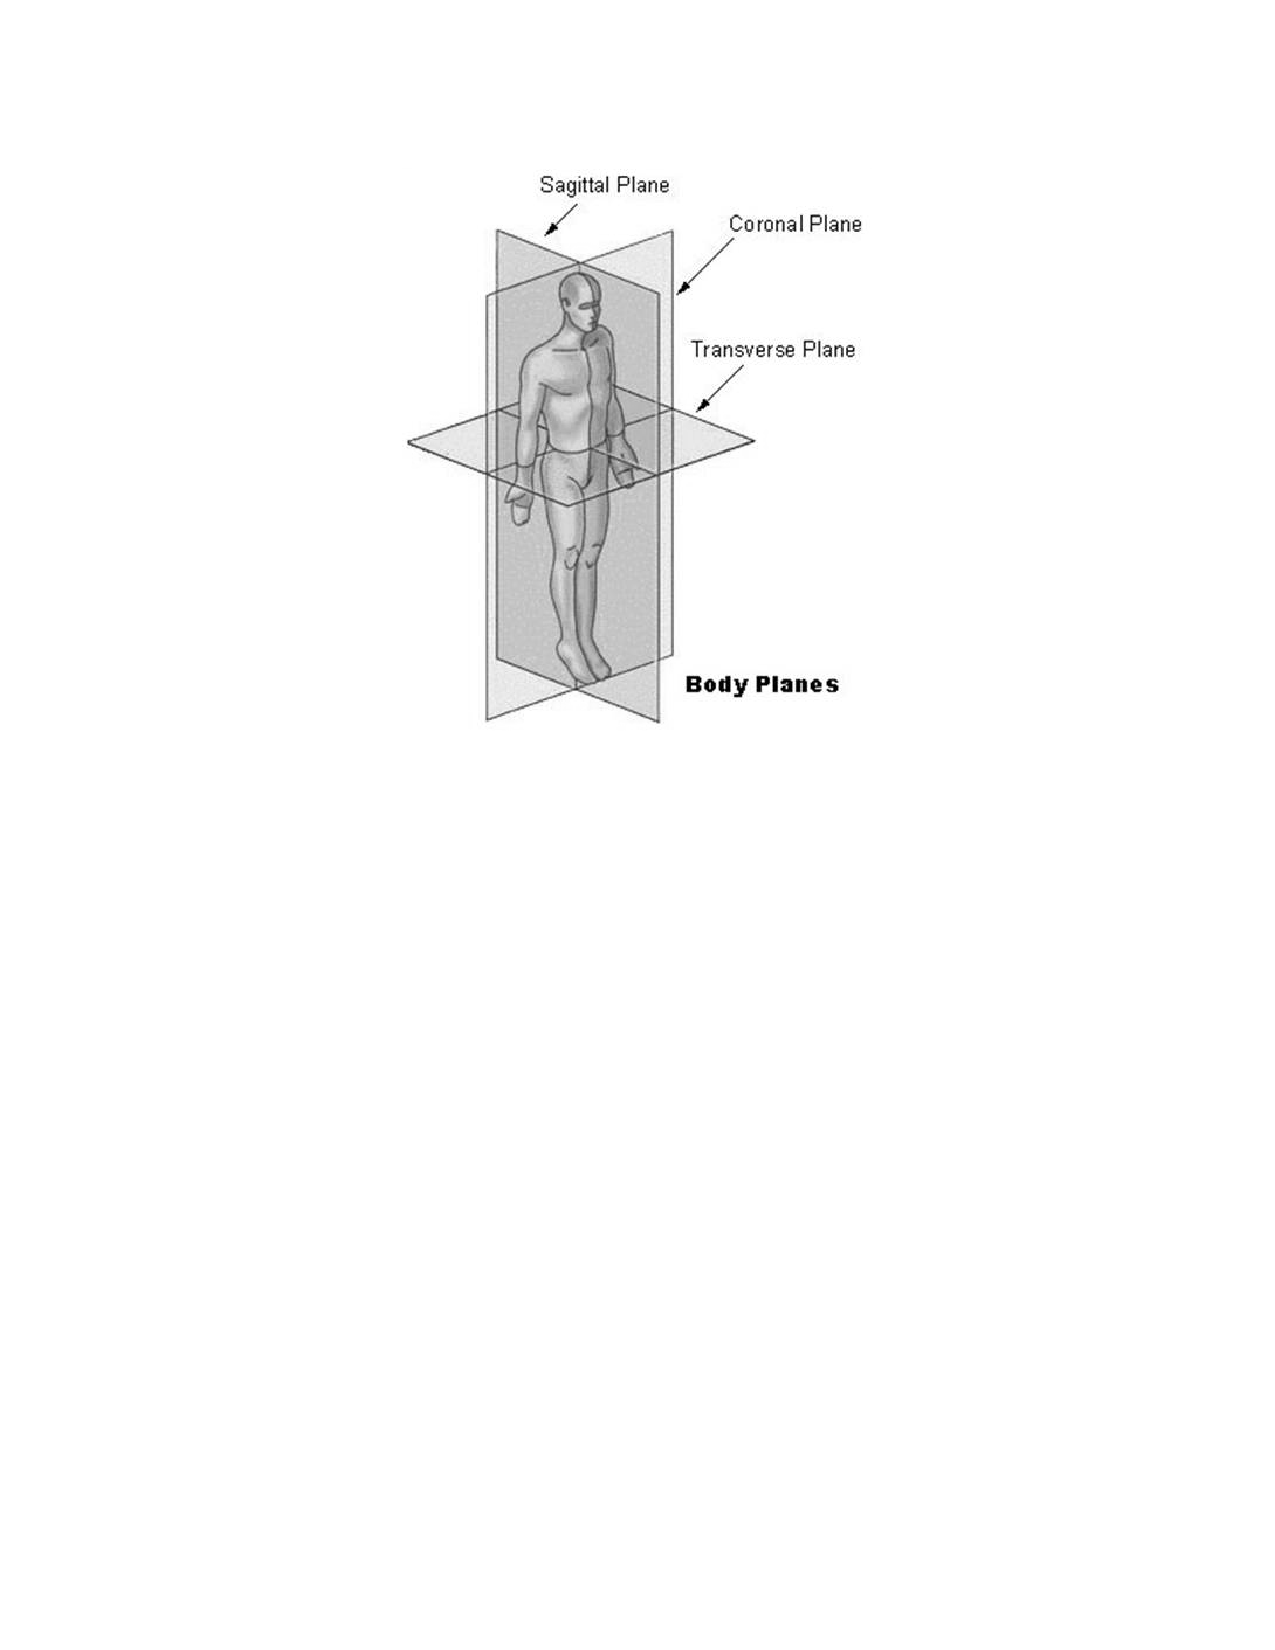
\includegraphics[height=4cm]{bodyplanes}
        \end{figure}
      \end{column}
      \begin{column}{0.6\textwidth}
        \begin{figure}
          \centering
          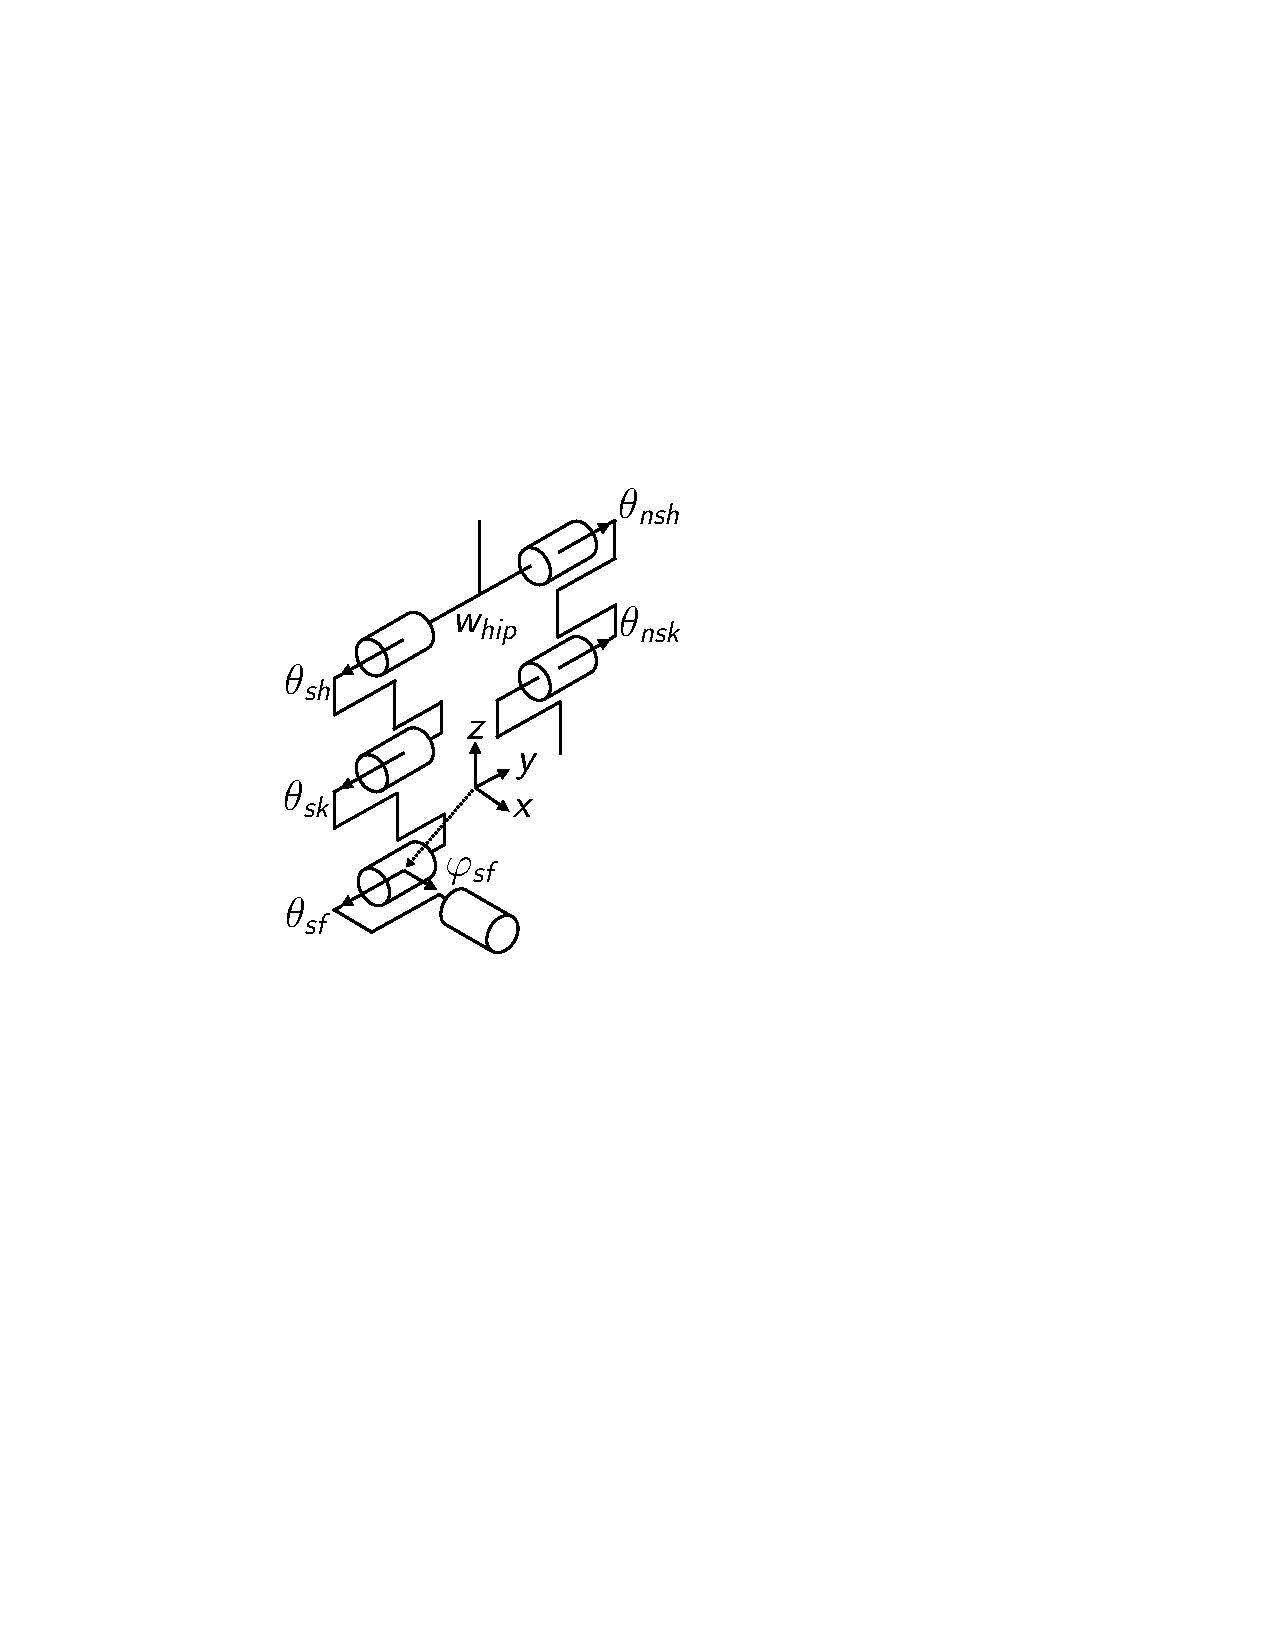
\includegraphics[height=3cm]{robot_angles_3d} \qquad
          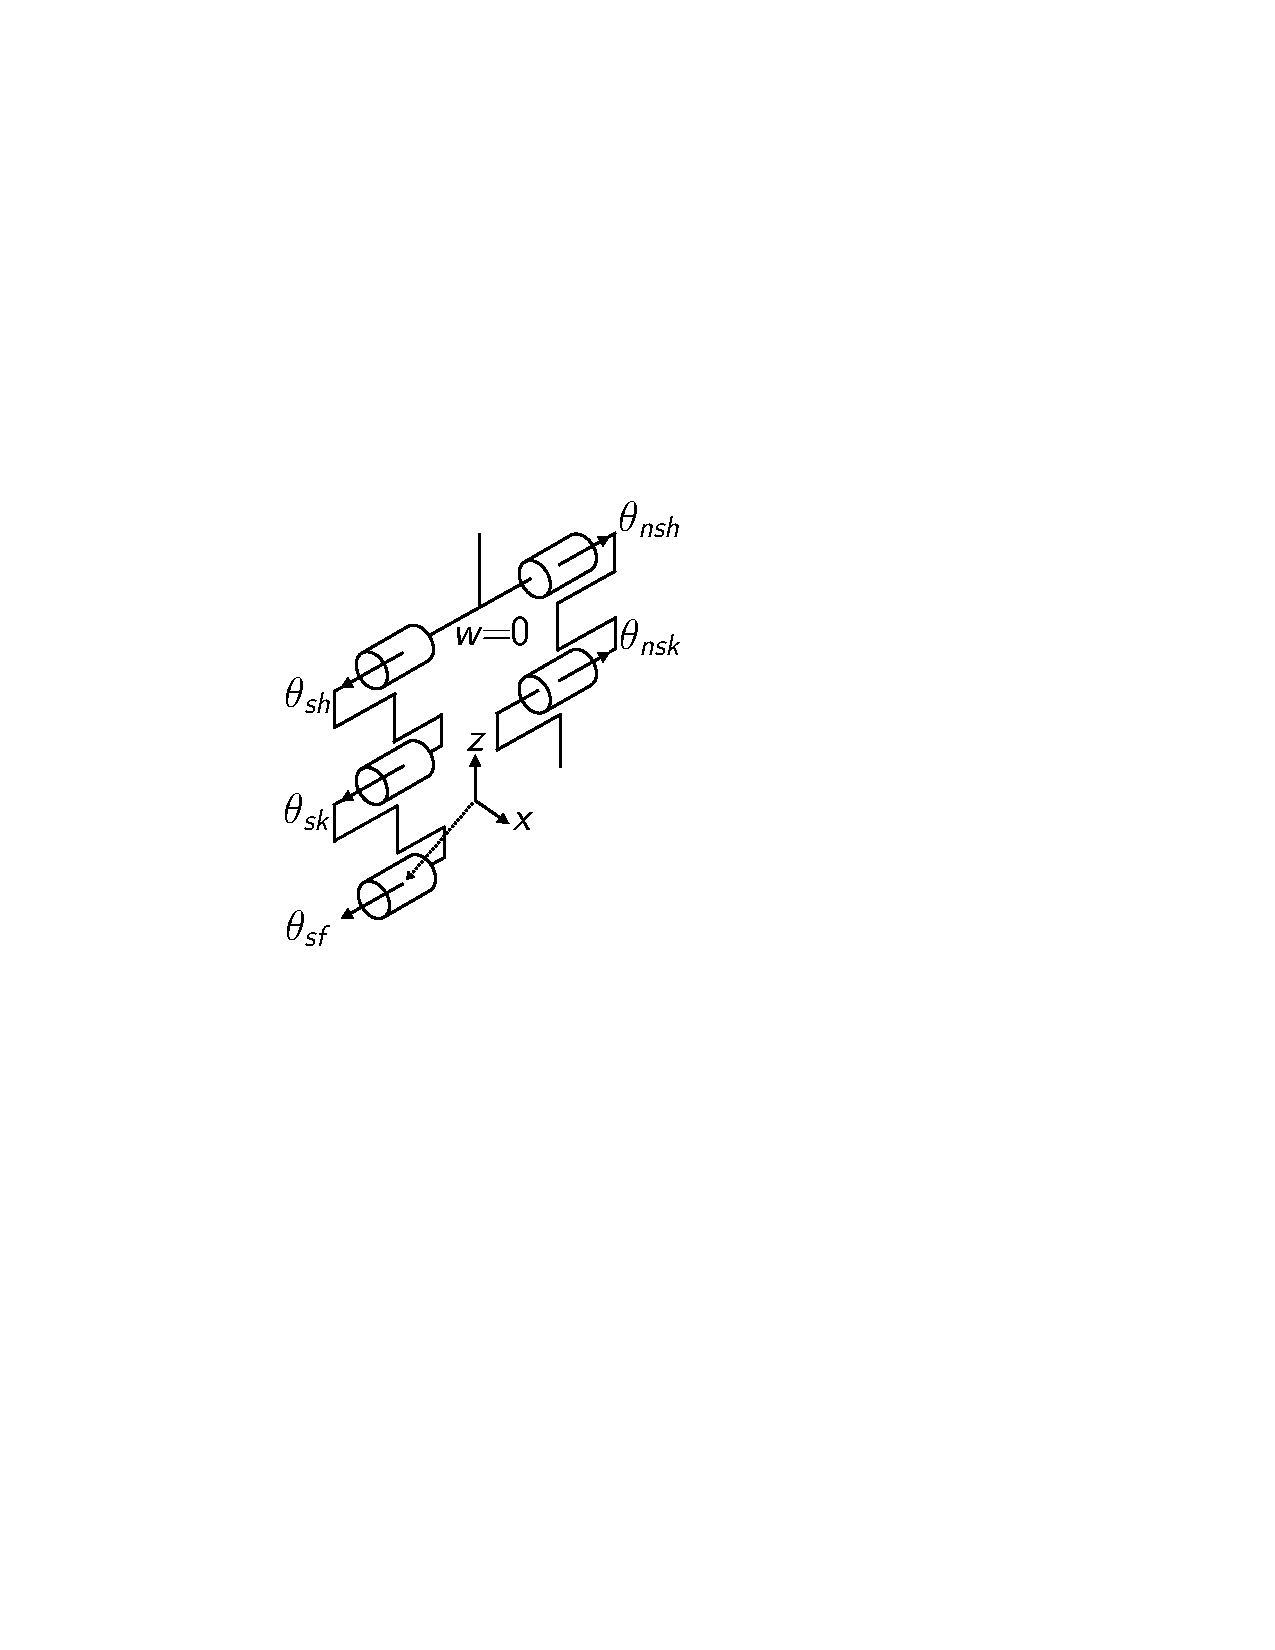
\includegraphics[height=3cm]{robot_angles_2d}
          \caption{Sagittal restriction of of 3D biped leads to a reduced model.}
        \end{figure}
      \end{column}
    \end{columns}
  }

  \only<2> {
    {\scriptsize  \textcolor{gray}{
        \begin{diagram}[width=5em,height=5em]
          \textcolor{black}{\fbox{$\begin{array}{c}$Hipped 3D Biped$\end{array}$}} &
          \rTo^{1^{\mathsf{st}} \:\: \mathsf{Reduction}}_{\mathsf{Control} \:\: \mathsf{Law}} &
          \fbox{$\begin{array}{c}$3D Biped$\\$with shaped$\\$energy$\end{array}$} &
          \rTo^{2^{\mathsf{nd}} \:\: \mathsf{Reduction}}_{\mathsf{Control} \:\: \mathsf{Law}} &
          \fbox{$\begin{array}{c}$3D Biped$\\$walking stably$\end{array}$}\\
          \dDashto^{\textcolor{black}{\mathsf{Sagittal}}}_{\textcolor{black}{\mathsf{Restriction}}} &&
          \uTo \dTo_{\begin{array}{c}$Reduction$\end{array}}&&\\
          \textcolor{black}{\fbox{$\begin{array}{c}$2D Biped$\end{array}$}} &
          \rTo^{\textcolor{black}{\mathsf{Sagittal}}}_{\textcolor{black}{\mathsf{Control} \:\: \mathsf{Law}}} &
          \textcolor{black}{\fbox{$\begin{array}{c}$2D Biped$\\$walking stably$\end{array}$}} && \\
    \end{diagram}}}
  }

  \only<3> {
    \begin{itemize}
    \item  The Lagrangian of the 3D biped has the general form:
      \begin{eqnarray}
        \label{eq:submats}
        \lefteqn{\Lfd(\cq{},\cdq{}) = -\Vu \ + }\\
        \nonumber
        &&\frac{1}{2}
        \left(\begin{array}{c c}
          \dot{\theta}^T & \dot{\varphi}
        \end{array}\right)
        \underbrace{\left(\begin{array}{c c}
            \Mth & \Mphitheta^T(\theta,\varphi)\\
            \Mphitheta(\theta,\varphi) & \Mphi(\theta,\varphi)
          \end{array}\right)}_{\mMu}
        \left(\begin{array}{c}
          \dot{\theta}\\
          \dot{\varphi}
        \end{array}\right), \nonumber
      \end{eqnarray}
      \vspace{-5mm}

    \item The Lagrangian of the sagittal restriction is given by:
      \begin{align*}
        \Lrd(\theta,\dot{\theta}) = \frac{1}{2} \dot{\theta}^T \Mth \dot{\theta} - \left.\Vu\right\vert_{\varphi=0},
      \end{align*}

    \end{itemize}
  }

  \only<4> {
    \vspace{-.1cm}
    \begin{itemize}

    \item The Lagrangian of the sagittal restriction is given by:
      \begin{align*}
        \Lrd(\theta,\dot{\theta}) = \frac{1}{2} \dot{\theta}^T \Mth \dot{\theta} - \left.\Vu\right\vert_{\varphi=0},
      \end{align*}

    \item This yields a control system: $(\fr,\gr)$.

    \item \alert{Assume} there exists a control law, $\usagarg$, that results in stable 2D waking for the dynamical system:
      \begin{align*}
        \flt = \fr(\theta, \dot{\theta}) + \gr(\theta) \usagarg.
      \end{align*}

    \end{itemize}
  }

  %\only<5> {
  %  \begin{figure}
  %    \centering
  %    \movie[width=0.6\textwidth,externalviewer]{
  %    \includegraphics[width=0.6\textwidth]{2dwalkinggait.pdf}}{Movies/2d-movie.avi}\\
  %    \includegraphics[height=0.3\textheight]{pp-2d-legs.pdf}
  %    \includegraphics[height=0.3\textheight]{pp-2d-feet.pdf}
  %  \end{figure}
  %}
  %
}

\frame[t] {
  \frametitle{$1^{\mathsf{st}}$ Reduction Control Law: Lagrangian Shaping Controller}

  Shape the total energy of the 3D biped so that functional Routhian reduction can be applied and the reduced system is exactly the 2D system obtained from the first control law.

  {\scriptsize \textcolor{gray}{
      \begin{diagram}[width=5em,height=5em]
        \textcolor{black}{\fbox{$\begin{array}{c}$Hipped 3D Biped$ \end{array}$}} &
        \rTo^{\textcolor{black}{1^{\mathsf{st}} \:\: \mathsf{Reduction}}}_{\textcolor{black}{\mathsf{Control} \:\: \mathsf{Law}}} &
        \textcolor{black}{\fbox{$\begin{array}{c}$3D Biped$\\$with shaped$\\$energy$\end{array}$}} &
        \rTo^{2^{\mathsf{nd}} \:\: \mathsf{Reduction}}_{\mathsf{Control} \:\: \mathsf{Law}} &
        \fbox{$\begin{array}{c}$3D Biped$\\$walking stably$\end{array}$}\\
        \dDashto^{\textcolor{black}{\mathsf{Sagittal}}}_{\textcolor{black}{\mathsf{Restriction}}} &&
        \uTo \dTo_{\textcolor{black}{\begin{array}{c}$Reduction$\end{array}}}&&\\
        \textcolor{black}{\fbox{$\begin{array}{c}$2D Biped$\end{array}$}} &
        \rTo^{\textcolor{black}{\mathsf{Sagittal}}}_{\textcolor{black}{\mathsf{Control} \:\: \mathsf{Law}}} &
        \textcolor{black}{\fbox{$\begin{array}{c}$2D Biped$\\$walking stably$\end{array}$}} &&
      \end{diagram}
  }}
}


\frame[t] {
  \frametitle{$2^{\mathsf{nd}}$ Reduction Control Law: Zero Dynamics Controller}

  Use feedback linearization to stabilize to the surface of initial conditions for which the decoupling promised by functional Routhian Reduction is valid.

  {\scriptsize  \textcolor{gray}{
      \begin{diagram}[width=5em,height=5em]
        \textcolor{black}{\fbox{$\begin{array}{c}$Hipped 3D Biped$\end{array}$}} &
        \rTo^{\textcolor{black}{1^{\mathsf{st}} \:\: \mathsf{Reduction}}}_{\textcolor{black}{\mathsf{Control} \:\: \mathsf{Law}}} &
        \textcolor{black}{\fbox{$\begin{array}{c}$3D Biped$\\$with shaped$\\$energy$\end{array}$}} &
        \rTo^{\textcolor{black}{2^{\mathsf{nd}} \:\: \mathsf{Reduction}}}_{\textcolor{black}{\mathsf{Control} \:\: \mathsf{Law}}} &
        \textcolor{black}{\fbox{$\begin{array}{c}$3D Biped$\\$walking stably$\end{array}$}}\\
        \dDashto^{\textcolor{black}{\mathsf{Sagittal}}}_{\textcolor{black}{\mathsf{Restriction}}} &&
        \uTo \dTo_{\textcolor{black}{\begin{array}{c}$Reduction$\end{array}}}&& \\
        \textcolor{black}{\fbox{$\begin{array}{c}$2D Biped$\end{array}$}} &
        \rTo^{\textcolor{black}{\mathsf{Sagittal}}}_{\textcolor{black}{\mathsf{Control} \:\: \mathsf{Law}}} &
        \textcolor{black}{\fbox{$\begin{array}{c}$2D Biped$\\$walking stably$\end{array}$}}&&
      \end{diagram}
  }}
}
}{}
\ifdefstring{\PRELIMSECE}{1}{\section{Human-Inspired Control}
\showtoc

\subsection{Human-Inspired Control Framework}
\frame{
  \frametitle{Human Data Experiment}
  \begin{columns}
    \begin{column}{0.65\textwidth}
      \begin{figure}
        \centering
        \vspace{-1cm}
        \caption{Experimental setup showing sensor placement for human data acquisition}
        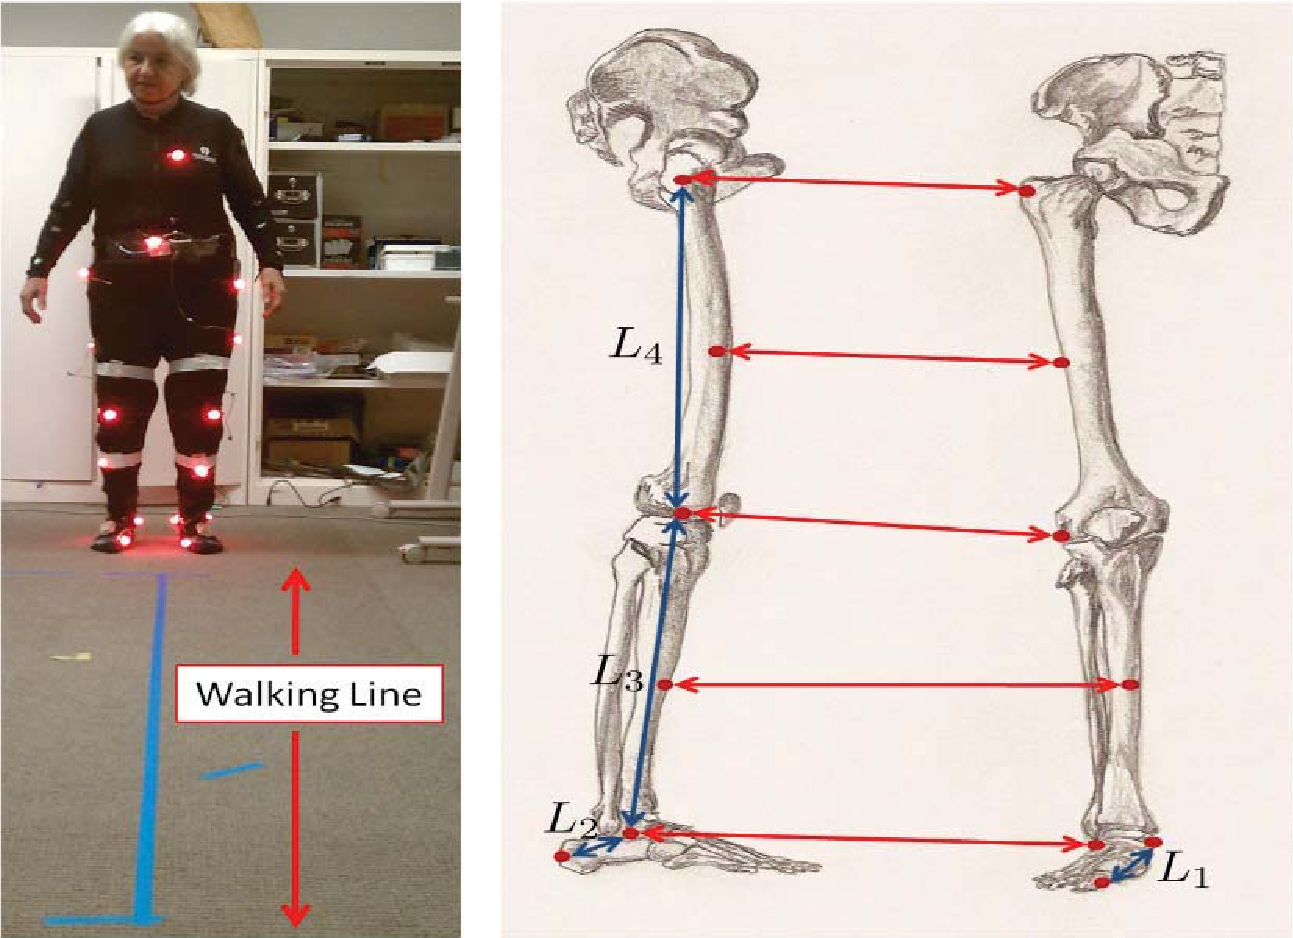
\includegraphics[width=1.0\columnwidth]{labeled_diagram}
      \end{figure}
    \end{column}
    \begin{column}{0.35\textwidth}
      \begin{figure} \centering
        \vspace{-1cm}
        \caption{Human outputs}
        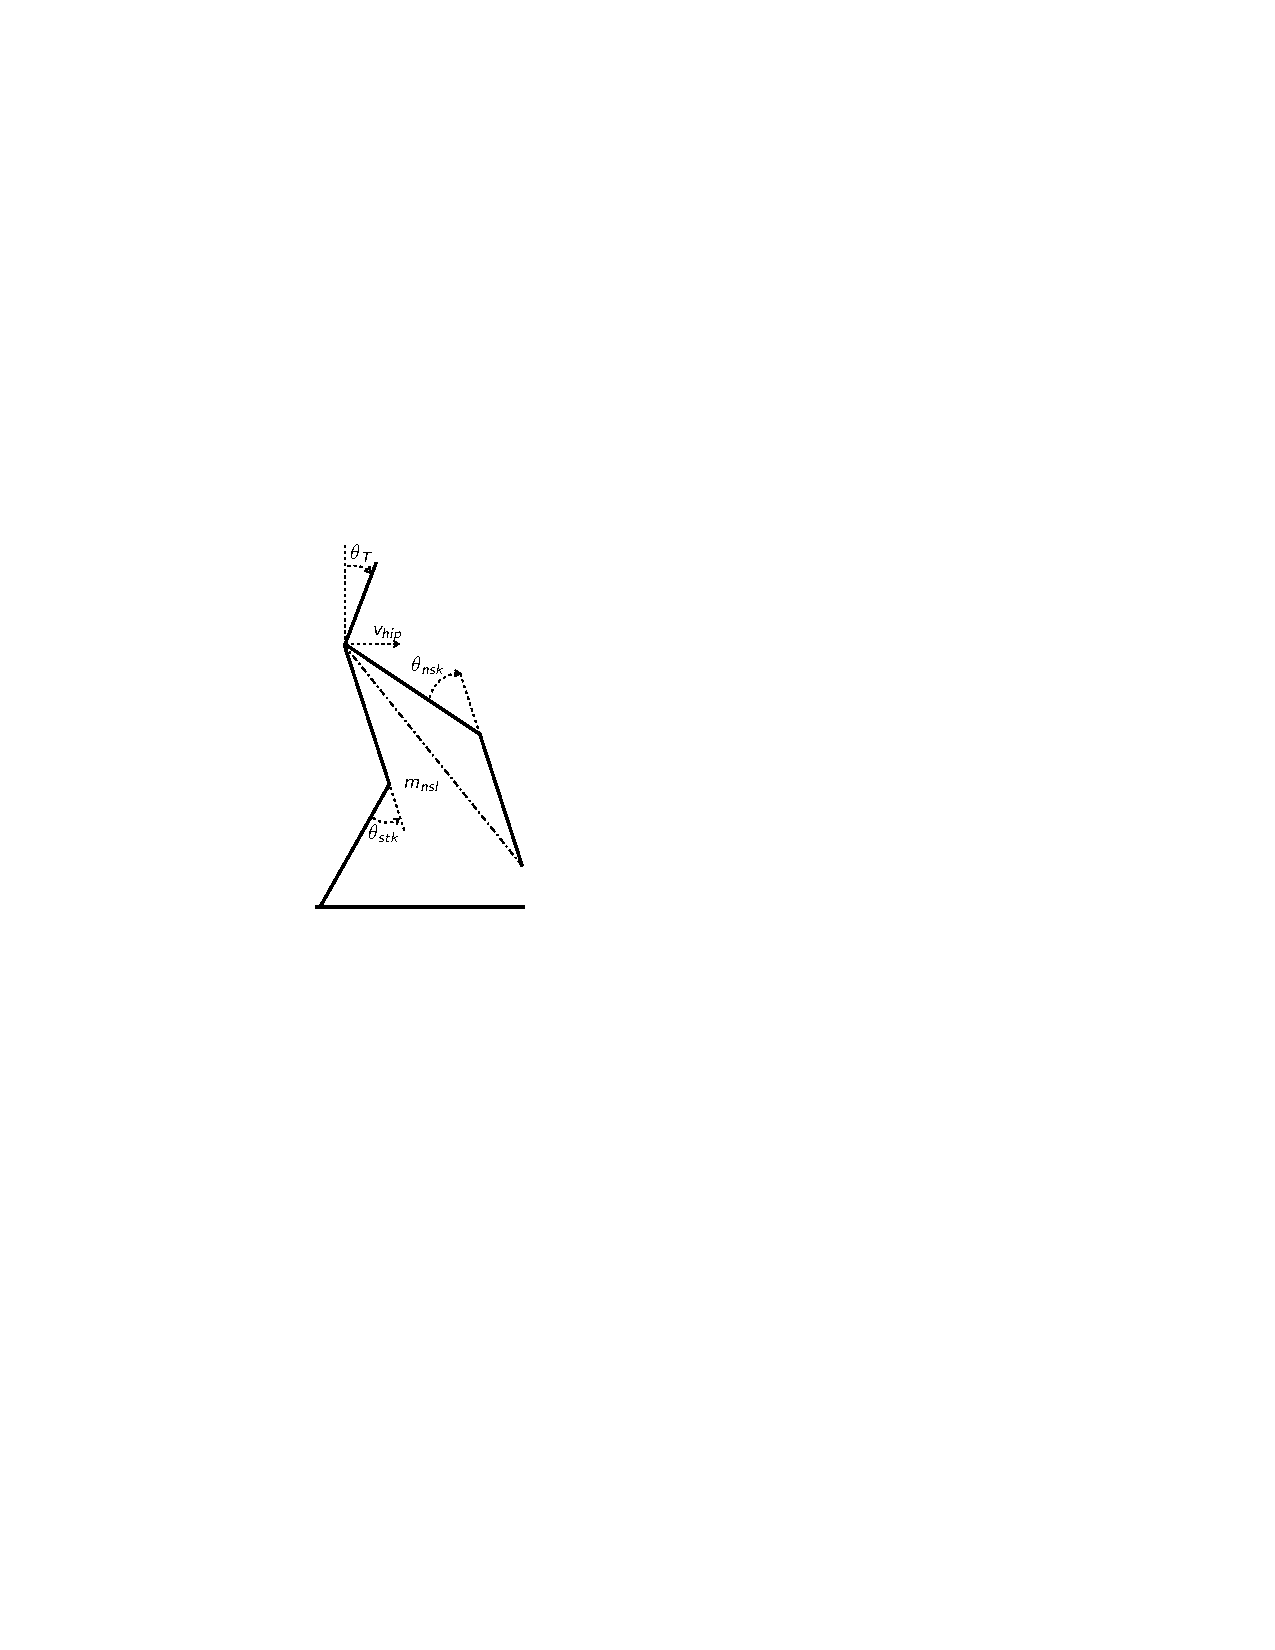
\includegraphics[width=0.8\columnwidth]{pointfoot_robot_const}
      \end{figure}
    \end{column}
  \end{columns}
}

\frame[t]{
  \frametitle{Canonical Walking Functions}
  The following function, termed the \blue{canonical walking function}, fits human kinematics data quite accurately:
  \begin{align}
    \nonumber
    y(t) &= e^{-\zeta \omega_{n} t} (c_{1} \cos (\omega_{d} t) + c_{2} \sin (\omega_{d} t)) + \hat{g}\\
    \tag{CWF}
    \label{eq:cwf}
    y^{H}(t, A)&= e^{-a_{3} t} (a_{1} \cos (a_{2} t) + a_{4} \sin (a_{2} t)) + a_{5}
  \end{align}
  where,
  \begin{itemize}
  \item
    $\zeta$ is the damping ratio,
  \item
    $\omega_{n}$, $\omega_{d}$ are the natural and damped natural frequencies, resp.,
  \item
    $c_{1}$ and $c_{2}$ are initial conditions,
  \item
    and $\hat{g}$ is from a particular solution for constant forcing.
  \end{itemize}
  Parameterize time using hip position:
  \begin{align*}
    \tau(\theta) := \frac{p_\mathit{hip}^{x}(\theta) - p_\mathit{hip}^{x}(\theta^{-})}{v_\mathit{hip}}
  \end{align*}
}

\begin{frame}[t]
  \frametitle{Example: 5-Link Biped}
  \begin{columns}
    \column{1.5in}
    Dynamic Model:
    \begin{align*}
      M(q) \ddot q + H(q, \dot q) = B(q) u
    \end{align*}
    \column{1.5in}
    \begin{figure}
      \centering
      \def\svgwidth{1.0\columnwidth}
      \input{../figs/cg2d-5link-model.eps_latex}
      \vspace{-2em}
      \caption{5-link biped configuration.}
    \end{figure}
  \end{columns}
\end{frame}

\frame{
  \frametitle{Selecting Human Outputs}
  The following human kinematics outputs are viable:
  \begin{enumerate}
    {
    \item[\HF{1}:] $\Oa$, \blue{forward hip velocity}, i.e., the velocity of the $x$-position of the hip,
    \item[\HF{2}:] $\Ob$, \blue{swing leg slope}, i.e., the tangent of the angle between the $z$-axis and the projection of the line connecting the swing ankle and hip,
    \item[\HF{3}:] $\Oc$, \blue{stance knee relative angle},
    \item[\HF{4}:] $\Od$, \blue{swing knee relative angle},
    \item[\HF{5}:] $\Oe$, \blue{vertical torso angle}, the angle of the torso measured with respect to the vertical axis of the world frame.
    }
  \end{enumerate}

  \vspace{1mm}
  For convenience, define the actual and desired outputs:
  \vspace{-1mm}
  \begin{align*}
    y_{1}^{a} = \Oa, \ y_{2}^{a} = \Ob, \ y_{3}^{a} = \Oc, \ y_{4}^{a} = \Od, \ y_{5}^{a} = \Oe,
  \end{align*}
  \vspace{-8mm}
  \begin{align*}
    y_{1}^{d} = y^{H}(\tau(\theta), A_1), \ \ldots, \ y_{5}^{d} = y^{H}(\tau(\theta), A_5)
  \end{align*}
}

\frame{
  \frametitle{Human-Inspired Optimization}
  The form of \eqref{eq:cwf} allows it to encode certain outputs:
  \vspace{-4mm}
  \begin{figure}
    \centering
    \caption{Canonical walking functions with parameters from \eqref{eq:opt}}
    \vspace{-2mm}
    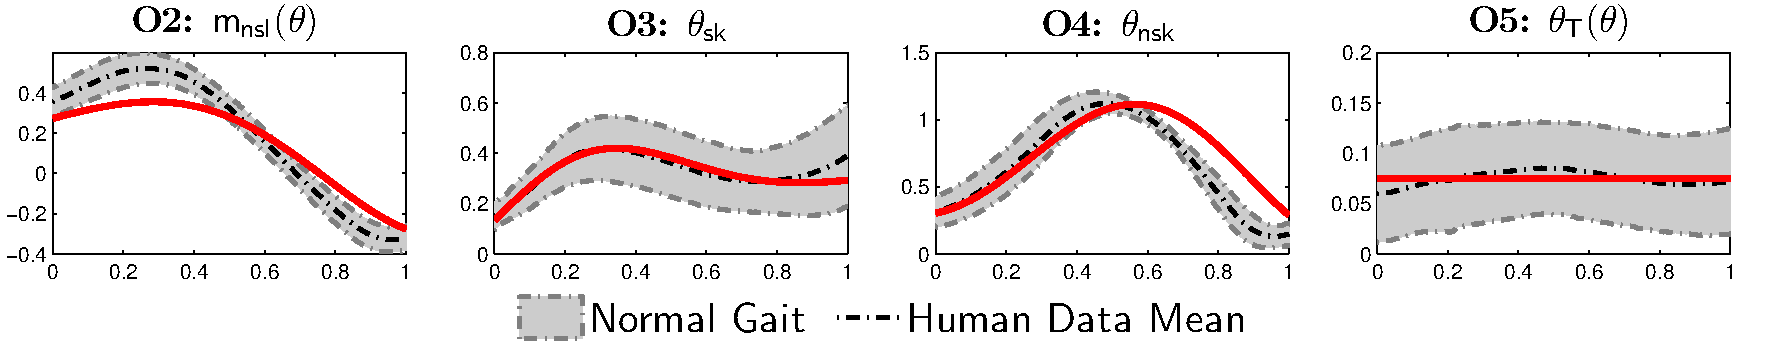
\includegraphics[width=1.0\textwidth]{human_function_fits}
    \vspace{-2mm}
  \end{figure}
  These outputs can be used to construct a \blue{partial hybrid zero dynamics} parameterized by matrix $A$ where outputs \textcolor{blue}{\HF{2}}--\textcolor{blue}{\HF{5}} of the robot are equal to the desired outputs for all time. The optimal parameters $A^*$ are found by solving
  \begin{align}
    \label{eq:opt}
    \tag{$\mathcal{O}$}
    A^{*} = \underset{A \in \R^{5 \times 5}}{\operatorname{argmin}} &  \:\: \mathrm{Cost}_{\mathrm{HD}}(A)  \\[-1mm]
    \nonumber
    \mathrm{s.t.} \quad & \ResetMapReduced(\GuardReduced \cap \HZD_{A}) \subset \PHZD_{A}
  \end{align}
}

\begin{frame}[t]
  \frametitle{Tracking the Partial Hybrid Zero Dynamics}
  Tracking can be accomplished with a variety of control schemes. PD control is interesting due to its model-independent nature:
  \begin{align*}
    \mathcal{K}_{2D}(\theta, \dot{\theta}) \! = \! k_p \left(\!\!
    \begin{array}{c}
      0\\
      y_{d,2} - y_{a,2}\\
      y_{d,3} - y_{a,3}\\
      y_{d,4} - y_{a,4}\\
      y_{d,5} - y_{a,5}
    \end{array}\!\!\right)  + 
    \blkdiag (k_p, k_d I_4)\left(\!\!
    \begin{array}{c}
      y_{d,1} - y_{a,1}\\
      \dot{y}_{d,2} - \dot{y}_{a,2}\\
      \dot{y}_{d,3} - \dot{y}_{a,3}\\
      \dot{y}_{d,4} - \dot{y}_{a,4}\\
      \dot{y}_{d,5} - \dot{y}_{a,5}
    \end{array}\!\!\right)
  \end{align*}

  This control law will result in walking in simulation (and in experiment in other works) and will satisfy assumptions made by functional Routhian reduction (introduced later).
\end{frame}

\begin{frame}[t]
  \frametitle{Procedure Summary}
  \begin{figure}
    \includemedia[
      width=0.8\columnwidth,
      height=0.45\columnwidth,
      addresource=human_experiment.mp4,
      activate=pageopen,
      flashvars={source=human_experiment.mp4&loop=true&autoPlay=true}
    ]{}{VPlayer9.swf}
    \caption{Human-inspired control produces robotic gaits from human data.}
  \end{figure}
\end{frame}

\begin{frame}[t]
  \frametitle{3D Simulation Results}
  \only<1>{
    \begin{figure}
      \centering
      \caption{Walking gait for 3D model with $v_\mathit{hip} = .6$ m/s}
      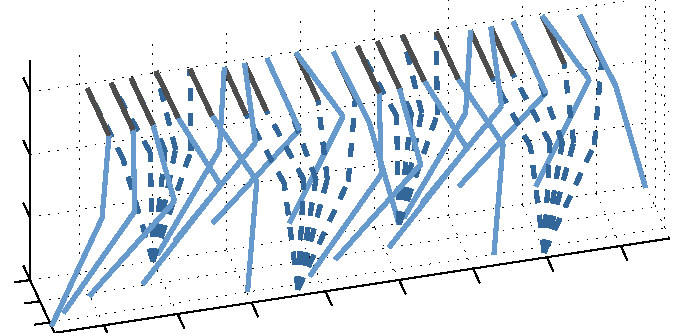
\includegraphics[width=.9\textwidth]{hic_frr_tiles_3d}
    \end{figure}
  }
  \only<2>{
    \begin{figure}
      \centering
      \caption{Phase portraits, human outputs, and actuator torques}
      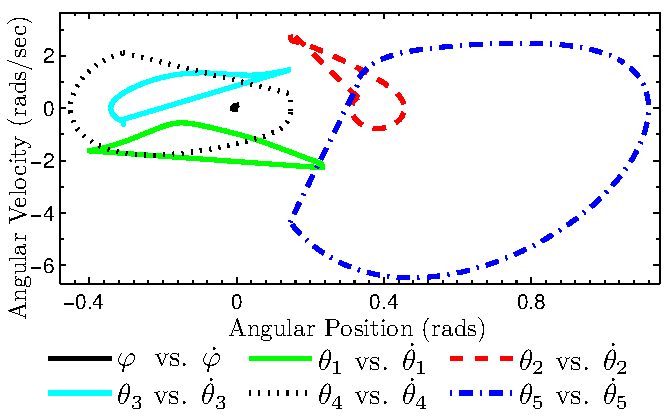
\includegraphics[width=.4\textwidth]{hic_frr_pp_3d_theta}\quad
      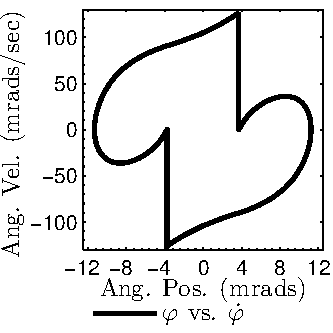
\includegraphics[width=.25\textwidth]{hic_frr_pp_3d_phi}\\[.3em]
      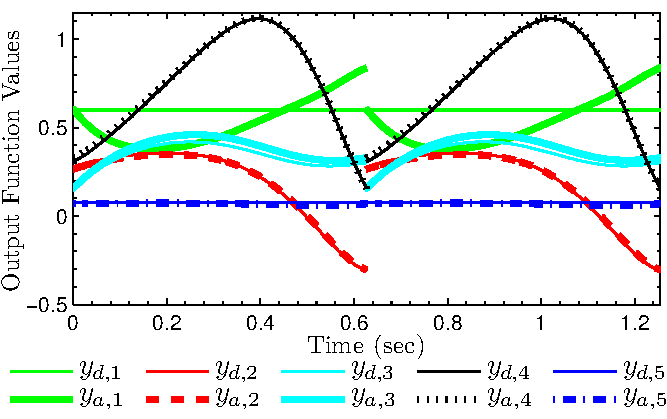
\includegraphics[width=.4\textwidth]{hic_frr_outputs_3d}\quad
      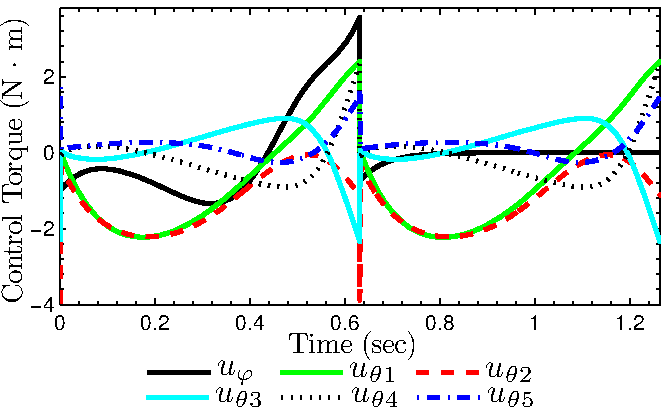
\includegraphics[width=.4\textwidth]{hic_frr_torques_3d}
    \end{figure}
  }
\end{frame}

\begin{frame}[t]
  \frametitle{3D Experiment Results}
  \begin{figure}
    \centering
    \caption{Experimental validation of HIC/FRR scheme}
    \only<1>{
      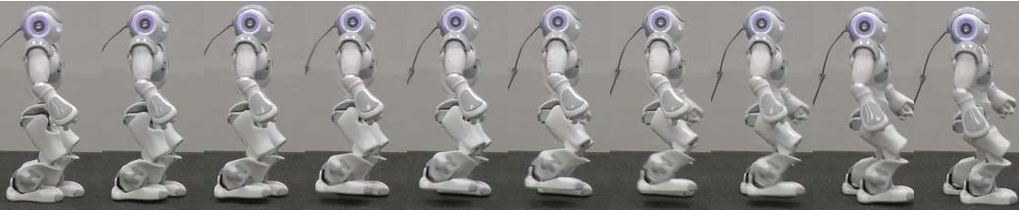
\includegraphics[height=2cm]{nao_tiles}\\[.3em]
      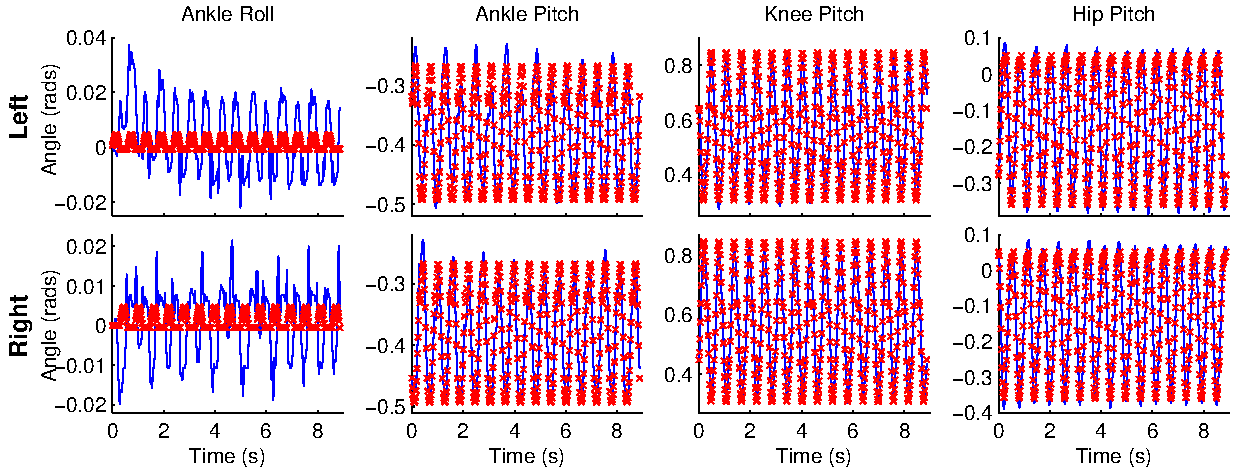
\includegraphics[height=3.25cm]{exp_angles}
    }
    \only<2>{
      \includemedia[
        %width=1.0\columnwidth,
        %height=0.5625\columnwidth,
        width=1.0\columnwidth,
        height=0.5\columnwidth,
        addresource=nao_reduction.mp4,
        activate=pageopen,
        flashvars={source=nao_reduction.mp4&loop=true&autoPlay=true}
      ]{}{VPlayer9.swf}
    }
  \end{figure}
\end{frame}

\begin{frame}[t]
  \frametitle{Combining ES and HIC}
  \only<1>{
    \begin{figure}
      \centering
      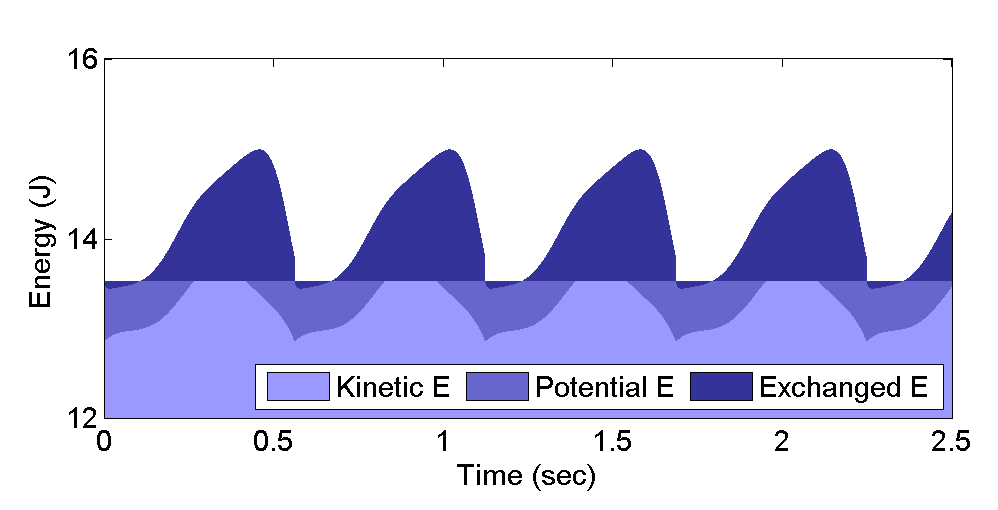
\includegraphics[width=1.0\columnwidth]{energy_conserved_5link}
      \caption{Demonstration of Energy Shaping and Human-Inspired Control.}
    \end{figure}
  }

  \only<2>{
    \begin{figure}
      \centering
      \includemedia[
        %width=1.0\columnwidth,
        %height=0.5625\columnwidth,
        width=1.0\columnwidth,
        height=0.5\columnwidth,
        addresource=5link_es.mp4,
        activate=pageopen,
        flashvars={source=5link_es.mp4&loop=true&autoPlay=true}
      ]{}{VPlayer9.swf}
      \caption{Energy shaping to stabilize to a gait from distant initial condition.}
    \end{figure}
  }
\end{frame}

}{}
\ifdefstring{\PRELIMSECF}{1}{\section{Conclusions}
\showtoc

\subsection{Remaining Work and Concluding Remarks}
\begin{frame}
  \frametitle{Current Results}
  \begin{itemize}
  \item 2D Compass-gait
  \item 2D 3-link
  \item 3D 3-link
  \item 2D 7-link
  \item 2D 5-link with HIC
  \end{itemize}
\end{frame}

\begin{frame}
  \frametitle{Remaining Work}
  \begin{itemize}
  \item 3D 5-link ES+HIC+FRR
  \item Formal proof of energy shaping
  \item 3D 7-link
  \item Application to SLIP model
  \end{itemize}
\end{frame}

\begin{frame}
  \frametitle{Questions}
  \Large{Questions?}
\end{frame}
}{}

%\section{Mechanics}
\showtoc

\subsection{Hybrid Systems}
\begin{frame}[t]
  \frametitle{Bipedal Models}
  \begin{figure}
    \centering
    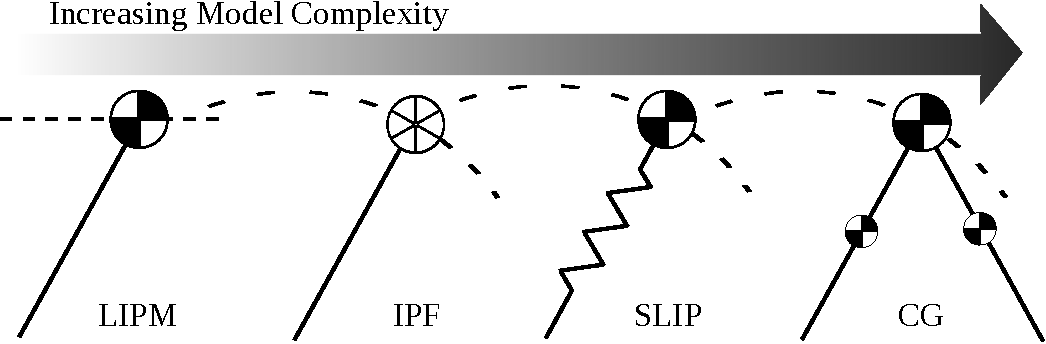
\includegraphics[width=.9\textwidth]{biped-models}
  \end{figure}
  \begin{itemize}
  \item Bipedal locomotion has been studied with a variety of models.
  \item Pendulum models consider massless legs with no impacts.
  \item Kinematic chains are markedly more complex than pendula.
  \end{itemize}
\end{frame}

\begin{frame}[t]
  \frametitle{Modeling Hybrid Systems}
  \begin{columns}
    \begin{column}{.63\textwidth}
      \begin{definition}
        A \alert{hybrid control system} is a tuple \vspace{-.3cm}
        $$\HCS = \hcsystem, \vspace{-.4cm}$$
        where
        \begin{itemize}
        \item
          $\Domain \subset \X$ is the \blue{domain of admissibility} with state space $\X$,
        \item
          $\ControlSet$ is a set of \blue{admissible controls},
        \item
          $\Guard$ is a \blue{guard} or \blue{switching surface},
        \item
          $\ResetMap$ is a smooth \blue{reset map},
        \item
          $(\xf, \xg)$ is a \blue{control system} on $\Domain$: \vspace{-3mm}
          \begin{align*}
            \dx = \xf(\x) + \xg(\x) \, \uu.
          \end{align*}
        \end{itemize}
      \end{definition}
    \end{column}
    \begin{column}{.4\textwidth}
      \begin{figure}    
        \centering
        \def\svgwidth{.8\columnwidth}
        \input{../figs/simple_hybrid_system.eps_latex}
      \end{figure}
      \vspace{-1em}
      A \alert{simple hybrid system}:\vspace{-.5em}
      $$\HS = \hsystem$$
    \end{column}
  \end{columns}
\end{frame}

\begin{frame}[t]
  \frametitle{Lagrangian Systems}
  Mechanical systems are defined by:
  \begin{itemize}
  \item Kinetic energy, $T : T\sQ \to \Rnn$,\\
  \item Potential energy, $U : \sQ \to \R$,
  \end{itemize}
  which together comprise the Lagrangian,
  \begin{align*}
    \Lagrangian\argsqdq = T\argsqdq - U\argsqdq.
  \end{align*}
  Dynamical motion in such a system with external forcing $\mathcal{F} = B\argsq u$ is governed by the Euler--Lagrange equation:
  \begin{align*}
    \frac{d}{dt} \pd{\Lagrangian}{\dq} - \pd{\Lagrangian}{\q} = B\argsq u.
  \end{align*}
\end{frame}

\begin{frame}[t]

  \frametitle{Swing Phase Dynamics}
  \begin{columns}
    \begin{column}{.55\textwidth}
      For Lagrangian $\Lagrangian$ with coordinates
      \begin{align*}
        \x = \argsqdq \in T\ConfigurationSpace,
      \end{align*}
      the dynamic model has the form
      \begin{align*}
        \M\argsq \, \ddq + \C\argsqdq \, \dq + \G\argsq = \B\argsq \, \uu,
      \end{align*}
      or $\dx = \xf\argsqdq+ \xg\argsq \, \uu,$ with
      \begin{align*}
        \xf\argsqdq &= \left(\!\!\begin{array}{c}
            \dq\\
            \M^{-1}\argsq (-\C\argsqdq \, \dq - \G\argsq)
          \end{array}\!\!\right),\\
        \xg(\q) &= \left(\!\!\begin{array}{c}
            \mathbf{0}_{m \times m}\\
            \M^{-1}(\q) \B(\q)
          \end{array}\!\!\right).
      \end{align*}
    \end{column}\!\!
    \begin{column}{.45\textwidth}
      \begin{figure}
        \centering
        \vspace{-10mm}
        \caption{Physical configuration}
        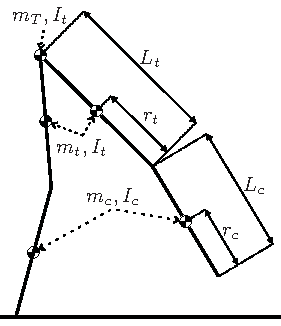
\includegraphics[width = 1.0\columnwidth]{pointfoot_robot_config}
      \end{figure}
    \end{column}
  \end{columns}
\end{frame}

\begin{frame}[t]
  \frametitle{Impact Dynamics}
  Introduce extended coordinates $\qe = (X, \q) \in \mathrm{SE}(3) \times \ConfigurationSpace$ which contains the kinematics of a reference point on the robot. Angular momentum balance based on H{\"u}rm{\"u}zl{\"u} and Marghitu:
  \begin{massump}
    \begin{itemize}
    \item Rigid-body plastic impacts
    \item Enough friction to prevent slipping
    \item Motors do not produce impulses
    \item No instantaneous change in configuration, i.e., $\qe^{-} = \qe^{+}$
    \end{itemize}
  \end{massump}
  Under these assumptions, the discrete dynamics satisfies
  \begin{align*}
    \left[\begin{array}{c c}
        \D_{e}(\qe) & -\Jacobian^{T}(\qe)\\
        \Jacobian(\qe) & \mathbf{0}_{3 \times 3}
      \end{array}\right]
    \left[\begin{array}{c}
        \dq^{+}\\
        \delta F(\qe, \dqe)
      \end{array}\right]
    = \left[\begin{array}{c c}
        \D_{e}(\qe) \, \dqe^{-}\\
        \mathbf{0}_{3}
      \end{array}\right].
  \end{align*}
\end{frame}

\subsection{Solutions to Hybrid Systems}
\begin{frame}[t]
  \frametitle{Hybrid Flows}
  A \alert{hybrid flow} of $\HS$ is a tuple
  \begin{align*}
    \chi^{\HS} = \left( \Delta, \mathscr{I}, \mathscr{C} \right),
  \end{align*}
  \vspace{-2em}
  \begin{itemize}
  \item $\Delta = \{0, 1, 2, \ldots\} \subseteq \Nat$ is a finite or infinite \blue{indexing set},
  \item $\mathscr{I} = \{I_{i} \}_{i \in \Delta}$ is a \blue{hybrid interval} where $I_{i} = [\tau_{i}, \tau_{i + 1}]$,
  \item $\mathscr{C} = \{c_{i} \}_{i \in \Delta}$ is a \blue{collection of solutions} of $\xf$, i.e., ${\dot c}_{i}(t) = \xf(c_{i}(t))$ $\forall i \in \Delta$.
  \end{itemize}

  \only<1>{
    \vspace{-1em}
    \begin{figure}
      \centering
      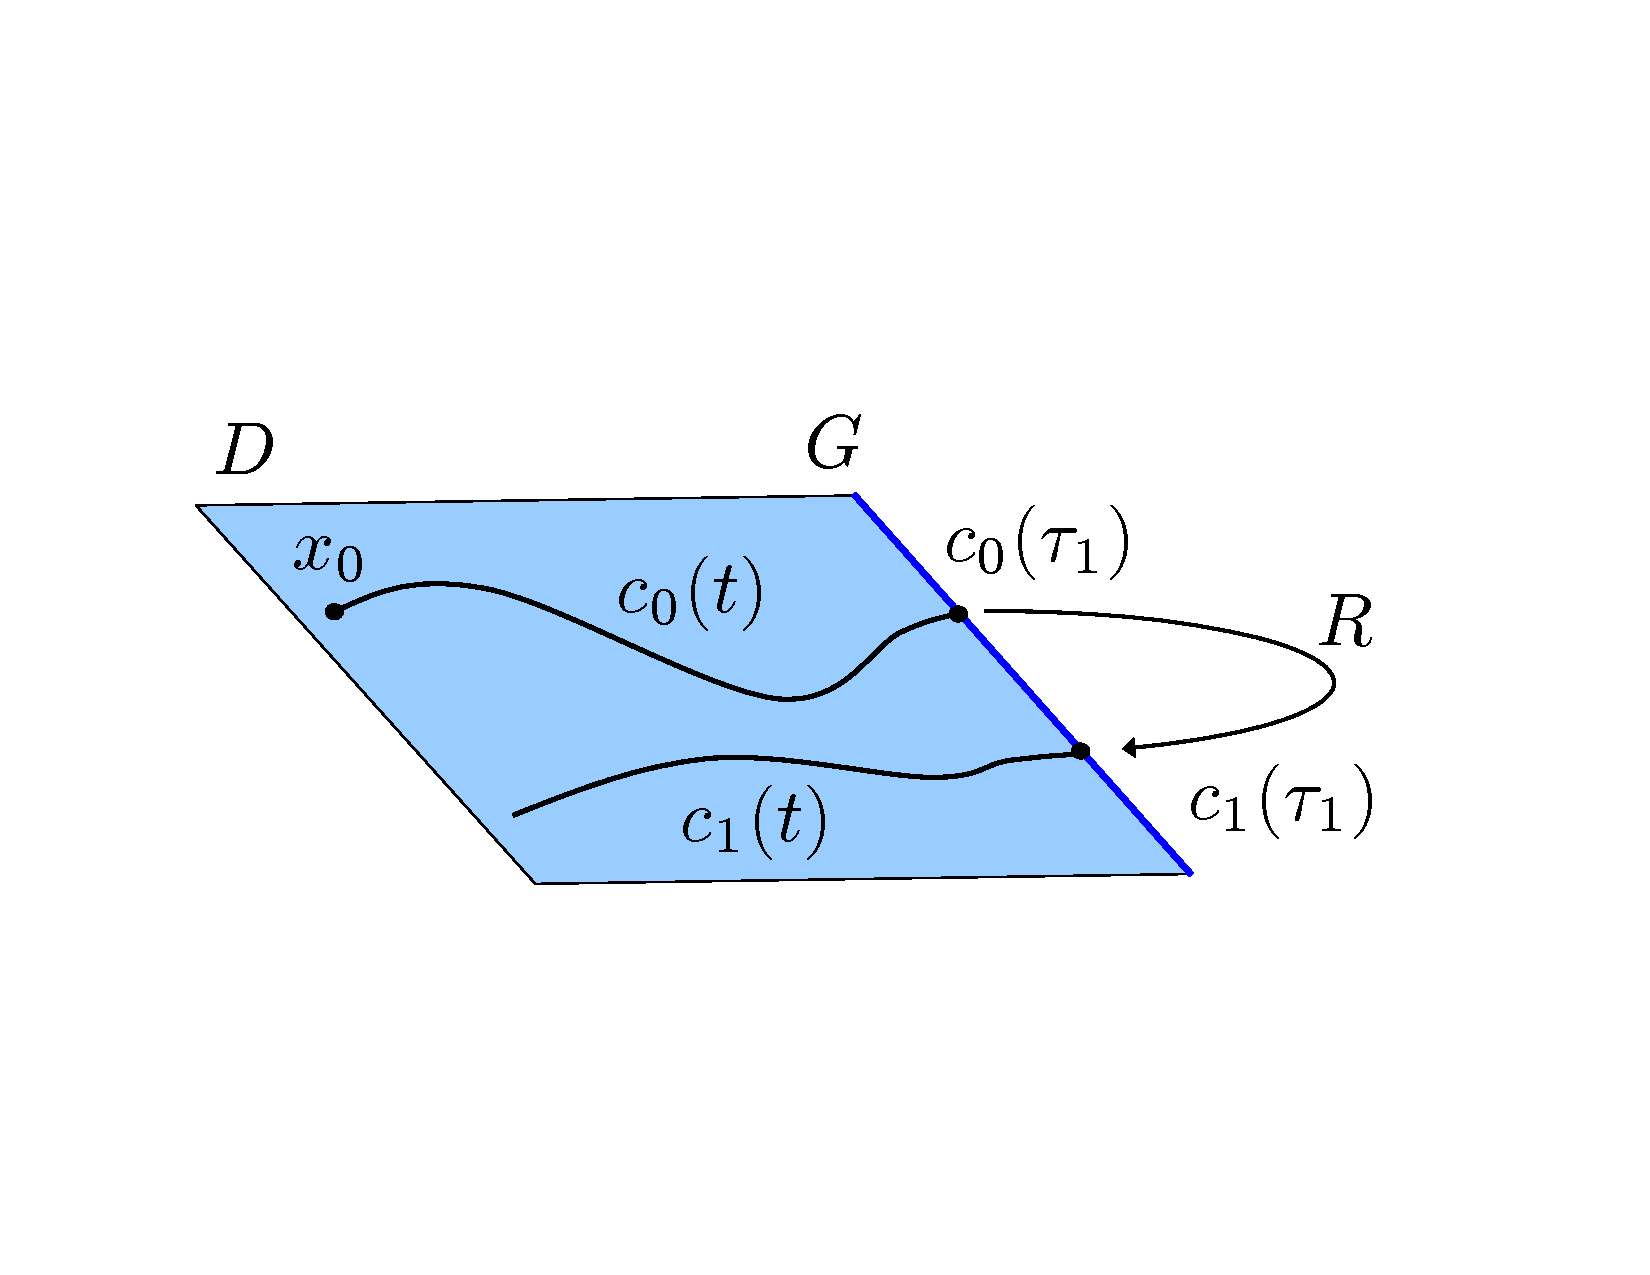
\includegraphics[width=0.5\columnwidth]{hybridflow}
    \end{figure}
    \vspace{-1em}
  }

  \only<2>{
    In addition, for every $i, i + 1 \in \Delta$, it is required that
    \begin{enumerate}
    \item $c_{i}(\tau_{i+1}) \in G$ and
    \item $\Delta(c_{i}(\tau_{i+1})) = c_{i+1}(\tau_{i+1})$
    \end{enumerate}
  }
\end{frame}


\begin{frame}[t]
  \frametitle{Periodic Orbits}
  \begin{figure}    
    \centering
    \def\svgwidth{.45\columnwidth}
    \input{../figs/hybrid_periodic_orbit.eps_latex}
    \caption{A hybrid periodic orbit. Stability is ascertained using the method of Poincar\'e.}
  \end{figure}
\end{frame}

\begin{frame}[t]
  \frametitle{Conservative Systems}
  For a conservative system, total energy is conserved; i.e.:
  \begin{align*}
    \Ec &= T\argsqdq + U\argsq\\
    &= \E(q(0), \dot q(0)) = \E_{0}
  \end{align*}
  Dynamical motion for such a system relies on the interplay between kinetic and potential energy, which is expressed in the Euler-Lagrange equation,
  \begin{align*}
    \frac{d}{dt} \pd{\Lagrangian}{\dq} - \pd{\Lagrangian}{\q} = 0.
  \end{align*}
\end{frame}


\begin{frame}[t]
  \frametitle{The Simplest Example: Passive Compass-Gait Biped}
  \only<1>{
    \begin{columns}
      \column{1.5in}
      Dynamic Model:
      \begin{align*}
        \M\argsq \ddot q + \CG\argsqdq = 0
      \end{align*}
      Control Law:
      \begin{align*}
        \uu = 0.
      \end{align*}
      \column{1.5in}
      \begin{figure}%width=1.0\columnwidth,
        
        \centering
        \def\svgwidth{1.0\columnwidth}
        \input{../figs/cg2d-slope-model.eps_latex}
        \vspace{-2em}
        \caption{Compass-gait biped falling down a slope.}
      \end{figure}
    \end{columns}
  }

  \only<2>{
    \begin{figure}
      \includemedia[
      % width=1.0\columnwidth,
      % height=0.5625\columnwidth,
      %width=1.0\columnwidth,
      %height=0.5\columnwidth,
      width=.9\columnwidth,
      height=0.45\columnwidth,
      addresource=cg2d_slope.mp4,
      activate=pageopen,
      flashvars={source=cg2d_slope.mp4&loop=true&autoPlay=true}
      ]{}{VPlayer9.swf}
      \caption{Stable passive gaits can be found for a range of slopes.}
    \end{figure}    
  }

  \only<3>{
    \begin{figure}
      \centering
      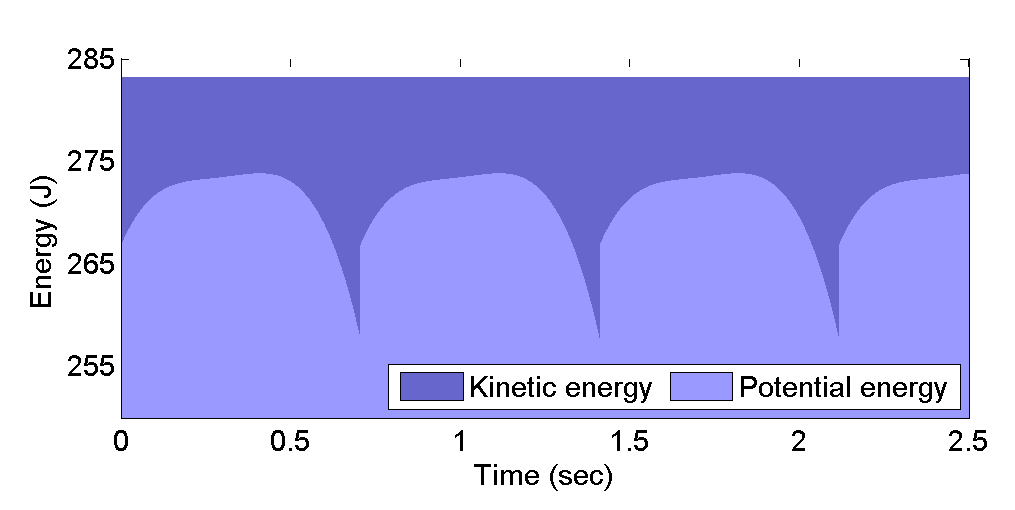
\includegraphics[width=1.0\columnwidth]{energy_cg2d_slope_model}
      \caption{Energy is exchanged between kinetic and potential in form.}
    \end{figure}    
  }
\end{frame}


\begin{frame}[t]
  \frametitle{Nonconservative Systems}
  For a nonconservative system, energy flows out of the system at a rate of $F_{\nc} \cdot dq$. Thus, the following quantity is conserved:
  \begin{align*}
    \Ec &= T\argsqdq + U\argsq - \int_{t_{0}}^{t} \! F_{\nc} \cdot \frac{dq}{d\tau} \ d\tau\\
    &= \E(q(0), \dot q(0)) = \E_{0}
  \end{align*}
  This equation expresses the interplay between kinetic and potential energy and the flow of energy into and out of the system.
\end{frame}


\begin{frame}[t]
  \frametitle{Example: Active Compass-Gait Biped}
  \only<1>{
    \begin{columns}
      \column{1.5in}
      Dynamic Model:
      \begin{align*}
        \M\argsq \ddq + \CG\argsqdq = \B\argsq \uu.
      \end{align*}
      Controlled Symmetries:
      \begin{align*}
        \uu &= \G\argsq - G(\Psi_{\gamma}\argsq)
      \end{align*}
      where $\Psi : \S \times \R \to \sQ$ rotates the frame of gravity by $\gamma$.

      \column{1.5in}
      \begin{figure}
        \centering
        \def\svgwidth{1.0\columnwidth}
        \input{../figs/cg2d-2link-model.eps_latex}
        \vspace{-2em}
        \caption{Compass-gait biped with Controlled Symmetries.}
      \end{figure}
    \end{columns}
  }
  \only<2>{
    \begin{figure}
      \includemedia[
      % width=1.0\columnwidth,
      % height=0.5625\columnwidth,
      width=.9\columnwidth,
      height=0.45\columnwidth,
      addresource=cg2d_2link_simulation.mp4,
      activate=pageopen,
      flashvars={source=cg2d_2link_simulation.mp4&loop=true&autoPlay=true}
      ]{}{VPlayer9.swf}
      \caption{Passive downhill gaits can be translated to flat ground with Controlled Symmetries.}
    \end{figure}    
  }
  \only<3>{
    \begin{figure}
      \centering
      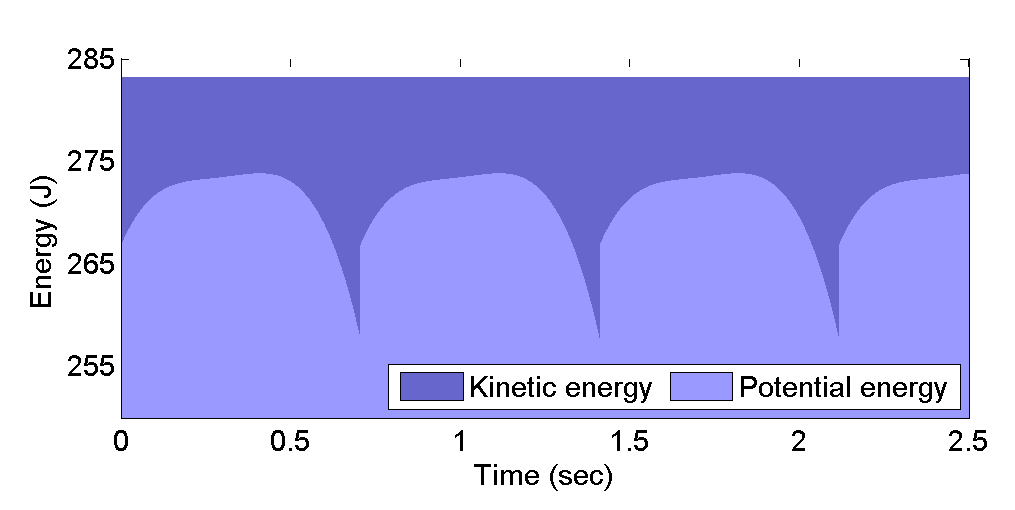
\includegraphics[width=1.0\columnwidth]{energy_cg2d_slope_model}
      \caption{Energy of the shaped system is conserved.}
    \end{figure}    
  }
\end{frame}

\begin{frame}[t]
  \frametitle{Example: 3-Link Biped}
  \only<1>{
    \begin{columns}
      \column{1.5in}
      Dynamic Model:
      \begin{align*}
        \M\argsq \ddq + \CG\argsqdq = \B\argsq \uu
      \end{align*}
      Control Law:
      \begin{align*}
        \uu &= \G\argsq - \G(\Psi\argsq)\\
        \uu_3 &=-k_{d} (\dot \vartheta_{T}^{a})\\
        &\hspace{1.8em} -k_{p} (\vartheta_{T}^{a} - \vartheta_{T}^{d})
      \end{align*}
      \column{1.5in}
      \begin{figure}
        \centering
        \def\svgwidth{1.0\columnwidth}
        \input{../figs/cg2d-3link-model.eps_latex}
        \vspace{-2em}
        \caption{3-link biped configuration.}
      \end{figure}
    \end{columns}
  }

  \only<2>{
    \begin{figure}
      \centering
      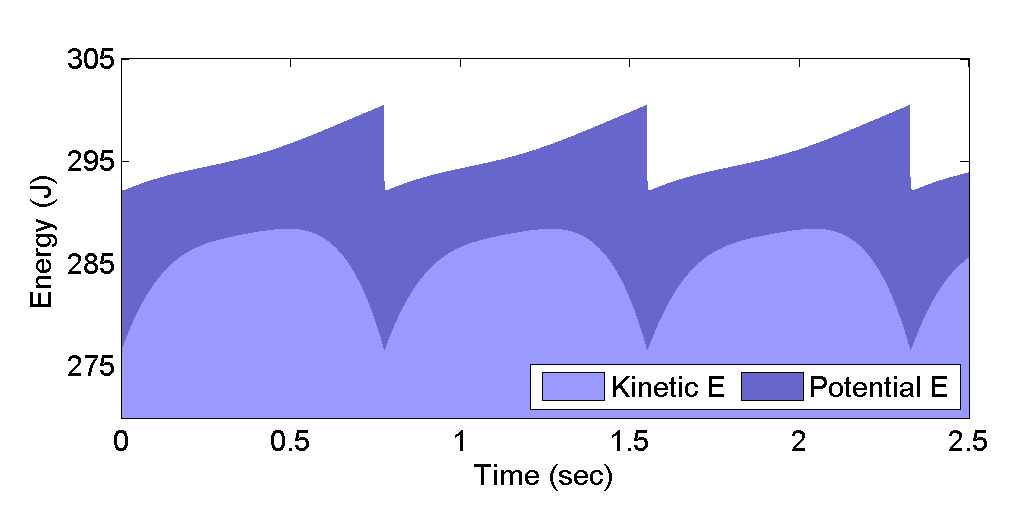
\includegraphics[width=1.0\columnwidth]{energy_cg2d_3link}
      \caption{Energy is not conserved as the controller injects energy.}
    \end{figure}
  }

  \only<3>{
    \begin{figure}
      \includemedia[
      %width=1.0\columnwidth,
      %height=0.5\columnwidth,
      width=.9\columnwidth,
      height=0.45\columnwidth,
      addresource=cg2d_3link_simulation.mp4,
      activate=pageopen,
      flashvars={source=cg2d_3link_simulation.mp4&loop=true&autoPlay=true}
      ]{}{VPlayer9.swf}
      \caption{Stable passive gaits can be found for a range of slopes.}
    \end{figure}
  }
\end{frame}

%\section{Energy Shaping}
\showtoc

\subsection{Energy Shaping with Control Lyapunov Functions}

\begin{frame}[t]
  \frametitle{Motivation}
  \begin{block}{Main Question}
    Can we use an understanding of energy exchange to improve robustness  of
    periodic orbits in hybrid mechanical systems?
  \end{block}

  \begin{block}{Observations}
    \begin{itemize}
    \item Numerous control design schemes exist for stabilizing hybrid mechanical
      systems to periodic orbits.
    \item Some controllers produce good behavior locally but lack robustness.
    \item Periodic orbits have associated energy functions with level sets which
      are invariant under the orbits.
    \end{itemize}
  \end{block}
\end{frame}

\begin{frame}[t]
  \frametitle{Overview}
  \begin{block}{Main Idea}
    Add robustness to a periodic behavior by imposing convergence on a conserved
    energy function, $\Ec : \x \to \R$, to a level set which is known to be
    invariant under the system dynamics.
  \end{block}
  
  \begin{block}{Control Objective}
    Choose control input $\mu\arx$ such that $\| \mu\arx \|$ is minimized and
    $\Ec\arxt \to \Eref$ as $t \to \infty$.
  \end{block}

  \begin{block}{Exponential Convergence}
    To achieve exponential stabilization, $\Ec\arxt$ should satisfy\vspace{-.4em}
    \begin{align*}
      \Ec\arxt \leq \Ec\arxzero e^{-\beta t} \mbox{ for } t \geq 0, \beta > 0.
    \end{align*}
  \end{block}
\end{frame}

\begin{frame}[t]
  \frametitle{Conserved Energy Functions}
  \only<1> {
    \begin{block}{Conservative Systems}
      A conservative system with state space $\x = \argsqdq$ is modeled as
      \begin{align*}
        \HCSbar = \left\{
          \begin{array}{l l}
            \left.\begin{array}{r c l}
                \hspace{.58em}\dx &=& \xfbar\argsqdq + \xgbar\argsq \, \uu
              \end{array}\right\}  & \mbox{if } \argsqdq \in \D \setminus \S,\\
            \left. \begin{array}{r c l}
                \qp &=& \Deltaq\argsqm\\
                \dqp &=& \Deltadq\argsqdqm
              \end{array} \right\} & \mbox{if } \argsqdq \in \S,
          \end{array}\right.
      \end{align*}
      where $\xfbar\argsqdq := \xf\argsqdq$ and $\xgbar\argsq := \xg\argsq$ for
      notational clarity. Total energy is conserved through the continuous
      dynamics, i.e.,
      \begin{align*}
        \Ec\argsqdq := T\argsqdq + U\argsq.
      \end{align*}
    \end{block}
  }

  \only<2> {
    \begin{block}{Nonconservative Systems}
      To properly handle the flow of energy due to $\vv\argsqdq$, define a storage
      function, $\W$, which obeys the differential equation
      \begin{align*}
        d\W = \vfR\argsqdq \, dt = \left( \B\argsq \, \vv\argsqdq \right)^{T}
        \frac{d\q}{dt}\art \, dt.
      \end{align*}
      Using $\W$, augment the state space, i.e., $\x := (\q, \dq, \W)$, and the vector
      fields (subsuming $\vv\argsqdq$ under $\xfbar\argsqdq$), i.e, 
      \begin{align*}
        \xfbar\argsqdq := \left(\begin{array}{c}
            \xf\argsqdq + \xg\argsq \, \vv\argsqdq\\
            \vfR\argsqdq
          \end{array}\right), &&
        \xgbar\argsq := \left(\begin{array}{c}
            \xg\argsq\\
            \boldzero
          \end{array}\right).
      \end{align*}
    \end{block}
  }
  \only<3> {
    \begin{block}{Nonconservative Systems}
      Use the augmented state to define the hybrid control system
      \begin{align*}
        \HCSbar = \left\{
          \begin{array}{l l}
            \left.\begin{array}{r c l}
                \hspace{1.15em}\dx &=& \xfbar\argsqdq + \xgbar\argsq \, \uu
              \end{array}\right\}  & \mbox{if } \argsqdq \in \D \setminus \S,\\
            \left. \begin{array}{r c l}
                \qp &=& \Deltaq\argsqm\\
                \dqp &=& \Deltadq\argsqdqm\\
                \Wp &=& \DeltaW = 0
              \end{array} \right\} & \mbox{if } \argsqdq \in \S.
          \end{array}\right.
      \end{align*}
      For such a system, the following quantity is conserved:
      \begin{align*}
        \Ec\argsqdqW := T\argsqdq + U\argsq - W.
      \end{align*}
    \end{block}
  }
\end{frame}

\begin{frame}[t]
  \frametitle{Rapidly Exponentially Stabilizing CLFs}
  A \blue{rapidly exponentially stability control Lyapunov function (RES--CLF)}
  $\Ve : \X \to \Rnn$ satisfies
  \begin{align*}
    &c_{1} \nx^{2} \leq \Ve\arx \leq \frac{c_{2}}{\resclfparam^{2}} \nx^{2},\\
    &\inf_{\uu \in \U} \Lie{\xfbar}\Ve\arx + \Lie{\xgbar}\Ve\arx \, \uu +
    \frac{c_{3}}{\resclfparam} \Ve\arx \leq 0
  \end{align*}
  for $c_{1}, c_{2}, c_{3} > 0$ exhibits exponential convergence. If the above
  are satisfied, then it is also true that
  \begin{align*}
    \left\| \pd{\Ve\arx}{\x} \right\| \leq c_{4} \nx.
  \end{align*}
\end{frame}

\begin{frame}[t]
  \frametitle{Energy Shaping}
  Consider a conserved energy function $\Ec\arx$ on a hybrid control system
  $\HCSbar$ which has a periodic orbit $\orbit$ and define a Lyapunov candidate:
  \begin{align*}
    V\arx = \frac{1}{2} \left(\Ec\arx - \Eref\right)^{2},
  \end{align*}
  with $\Eref$ the constant energy level of the system on the orbit
  $\orbit$. For a RES--CLF, we seek a feedback control law, $\mu\arx$, such that
  \begin{align*}
    \Lie{\xfbar} V\arx + \Lie{\xgbar} \V\arx \, \mu\arx + \epsilon \V\arx &\leq 0.
  \end{align*}
\end{frame}

\begin{frame}[t]
  \frametitle{Quadratic Program Formulation}
  The linear form of the RES--CLF condition suggests
  \begin{align}
    \nonumber
    \mueps\arx = \argmin_{\uu \in \R^{n}}  \, & \uu^T \uu,\\
    \mbox{s.t. } & \Aclf\arx \, \uu \leq \bclf\arx
  \end{align}
  which encodes the dynamics of the system. This controller imposes exponential
  stabilization of the energy as defined by the RES--CLF.
\end{frame}

\begin{frame}[t]
  \frametitle{Main Theorem}
  \begin{block}{Theorem [Energy Shaping]}
    Given an exponentially-stable cycle in a hybrid system, application
    of the energy shaping controller results in the closed-loop hybrid system
    \begin{align*}
      \HS_{\resclfparam} = \left\{
        \begin{array}{r c l l}
          \dx &=& \xfbar\arx + \xgbar\arx \, \mueps\arx, & \x \in \D \setminus \S,\\
          \xp &=& \Delta(\xm), & \x \in \S,
        \end{array}\right.
    \end{align*}
    which is exponentially stable about the hybrid periodic orbit $\orbit$ for
    large enough $\resclfparam$.
  \end{block}
\end{frame}

\subsection{Sketch of Proof}

\begin{frame}[t]
  \frametitle{Overview of Proof}
  \begin{block}{Sketch of Proof [Energy Shaping]}
    \begin{enumerate}
    \item Transform the coordinates into a more intuitive form.
    \item Define a discrete Lyapunov candidate function valid on the \Poincare{} map.
    \item Show the conditions for stability through bounding arguments.
    \end{enumerate}
  \end{block}
\end{frame}

\begin{frame}[t]
  \frametitle{Zero Dynamics Formulation}
  Construct a change of coordinates, splitting up the system into two sets of
  coordinates:
  \begin{align*}
    \dot \zdx &= f\argsxz + g\argsxz \, \uu,\\
    \dot \zdz &= q\argsxz + w\argsxz \, \uu.
  \end{align*}
  The vector fields $f$, $g$, $q$, and $w$ are assumed to be locally Lipschitz
  continuous. For simplicity, define
  \begin{align*}
    \bigF\argsxz = \left(\begin{array}{c}
        f\argsxz\\
        q\argsxz
      \end{array}\right),&&
    \bigG \argsxz = \left(\begin{array}{c}
        g\argsxz\\
        w\argsxz
      \end{array}\right).
  \end{align*}
\end{frame}

\begin{frame}[t]
  \frametitle{Energy-Based Coordinate Change}
  \only<1> {
    \begin{block}{Conservative Systems}
      Using the state $\x = \argsqdq$, construct the transformation
      $\xform\argsqdqW := \argsxz$ where
      \begin{align*}
        \zdx &= \Ec\argsqdq - \Eref,\\
        \zdz &= \xrem,
      \end{align*}
    \end{block}
  }

  \only<2> {
    \begin{block}{Nonconservative Systems}
      Using the state $\x = \argsqdqW$, construct the transformation
      $\xform\argsqdqW := \argsxz$ where
      \begin{align*}
        \zdx &= \Ec\argsqdqW - \Eref,\\
        \zdz &= \xremW,
      \end{align*}
    \end{block}
  }
  where $n$ is the size of the configuration space, $\Q$. The fixed point of the
  hybrid system is chosen to occur at $\argsxz = \xzst$ such that $\Delta\xzst =
  \argszero$.
\end{frame}

\begin{frame}[t]
  \frametitle{Validity of Transformation}
  \only<1> {
    \begin{block}{Conservative Systems}
      The coordinate change $\xform\arx = \xform\argsqdq$ is valid if it is locally
      diffeomorphic around the orbit $\orbit$, i.e., if
      \begin{align*}
        \pd{\xform\argsqdq}{\argsqdq} =
        \left(\begin{array}{c c}
            I_{2n-1} & \boldzero_{2n-1 \times 1}\\
            \pd{\Ec(\q, \dq)}{\xrem} & \pd{\Ec(\q, \dq)}{\dq_{n}}
          \end{array}\right)
      \end{align*}
      % 
      has full rank, which occurs when
      \begin{align*}
        \det\left(\pd{\xform\argsqdq}{\argsqdq}\right) =
        \pd{\Ec\argsqdq}{\dq_{n}} \ne 0.
      \end{align*}
    \end{block}
  }
  
  \only<2> {
    \begin{block}{Nonconservative Systems}
      The coordinate change $\xform\arx = \xform\argsqdqW$ is valid if it is
      locally diffeomorphic around the orbit $\orbit$, i.e., if
      \begin{align*}
        \pd{\xform\argsqdqW}{\argsqdqW} =
        \left(\begin{array}{c c c}
            I_{2n-1} & \boldzero_{2n-1 \times 1} & \boldzero_{2n-1 \times 1}\\
            \pd{\E\argsqdqW}{\xrem} & \pd{\Ec\argsqdqW}{\dq_{n}} & 1\\
            \boldzero_{1 \times 2n-1} & 0 & 1
          \end{array}\right)
      \end{align*}
      % 
      has full rank, which occurs when
      \begin{align*}
        \det \pd{\xform\argsqdqW}{\argsqdqW} = \pd{\Ec\argsqdqW}{\dq_{n}} \ne 0.
      \end{align*}
    \end{block}
  }
\end{frame}

\begin{frame}[t]
  \frametitle{Flows of Continuous Dynamical Systems}
  The flow of an ODE expressed in the variables $\argsxz$ is given
  by
  \begin{align*}
    \flowt\argsxz = \int_{0}^{t} \left[ \bigF\argsxztau + \bigG\argsxztau \,
      \uu\argsxztau \right] \, d\tau
  \end{align*}
  for some feedback control law $\uu : \zdX \times \zdZ \to \U$. For some stable
  tube $\stabletube$ around the orbit $\orbit$, it holds that the vector fields
  are bounded:
  \begin{align*}
    \supF & := \sup \left\{ \left\| \bigF\argsxz \right\| : \argsxz \in
      \stabletube \right\},\\
    \lambdamaxG &:= \sup \left\{\lambdamax\bigG\argsxz : \argsxz \in \stabletube
    \right\},\\
    \lambdaminG &:= \inf \left\{\lambdamin\bigG\argsxz : \argsxz \in \stabletube
    \right\}.
  \end{align*}
\end{frame}


\begin{frame}[t]
  \frametitle{Definition of the \Poincare{} Map}
  \only<1> {
    The \blue{\Poincare{} first return map} takes a point on the guard, applies
    the reset map and then integrates forward until the guard is reached
    again. For the shaped system, $\Pe : \S \to \S$, is defined by
    \begin{align*}
      \Pe\argsxz = \floweps_{\TIeDelta}\argsDeltaxz,
    \end{align*}
    where $\TIe : \zdX \times \zdZ \to \Rnn$ is the \tti{} function which is
    defined by
    \begin{align*}
      \TIe\argsxz = \inf \{ t \geq 0 : h(\flowepst\argsxz) \}
    \end{align*}
    and is locally Lipschitz continuous by the implicit function theorem.
  }

  \only<2> {
    \begin{figure}    
      \centering
      \def\svgwidth{.78\columnwidth}
      \input{../figs/poincare_return_map.eps_latex}
      \caption{The \Poincare{} map is defined by the \tti{} function and maps
        from states on the \Poincare{} section $\S$ back to the section.}
    \end{figure}
  }

  \only<3> {
    Using the change of coordinates $\rho(\resclfparam) :=
    \tfrac{1}{\resclfparam}$, define the function
    \begin{align*}
      N(t, \rho, \zdx, \zdz) = h(\flowrhot(\Deltaxz)),
    \end{align*}
    By the implicit function theorem, there exists a $\delta > 0$ and a unique
    function $\taurho(\rho, \zdx, \zdz)$ defined and locally Lipschitz for all
    $(\rho, \zdx, \zdz) \in \B_{\delta}(0, 0, \zdzst)$ such that $\tau^{0}(0,
    \zdzst) = \TI(0, \zdzst) = \Tst$ where $\Tst$ is the period of the invariant
    orbit $\orbit$.\\ \ \\

    Selecting a fixed $\resclfparam > 0$ with the min-norm controller, it
    follows that for some $\delta > 0$ and $\argsxz \in \B_{\delta}\xzst \cap
    \S$,
    \begin{align*}
      \label{eq:TIe-bounds}
      0.9 \Tst \leq \TIe\argsxz \leq 1.1 \Tst.
    \end{align*}
  }
\end{frame}

\begin{frame}[t]
  \frametitle{Equivalence of Hybrid Periodic Orbits}
  \begin{lemma}[Equivalence of Orbits]
    Applying the energy shaping controller to the hybrid control system $\HCSbar$
    results in the closed-loop hybrid system $\HSepsbar$ that demonstrates a
    periodic orbit which is identical to the unshaped system $\HSbar$.
  \end{lemma}
  \begin{block}{Proof}
    The energy of states $\xo \in \orbit$ is a constant,
    $\E(\xo) \equiv \Eref$. By the choice of Lyapunov function,
    $\V(\xo) \equiv 0$. In addition, $\dV(\xo) \equiv 0$ since
    the system is conservative. And since the solution to the optimization
    problem has cost $\uu^{T}(\xo) \uu(\xo) \equiv 0$, the
    control effort is also zero. Hence the orbits are equivalent.
  \end{block}
\end{frame}

\begin{frame}[t]
  \frametitle{Boundedness of \TtI{} Function}
  \only<1> {
    The difference in solutions between the shaped and unshaped systems can be
    bounded by examining the difference in solutions:
    \begin{lemma}[Boundedness of \TtI{}]
      For the hybrid systems $\HSbar$ and $\HSepsbar$,
      \begin{eqnarray}
        \nonumber
        &| \TIe(\Deltaxz) - \TI(\Deltaxz) | \leq \ATIe \nzdxzst,
      \end{eqnarray}
      where $\limeps \ATIe = 0$.
    \end{lemma}
  }
  
  \only<2> {
    \begin{block}{Proof (Boundedness of \TtI{})}
      Construct an auxiliary \tti{} function $\TB$ which is locally Lipschitz
      continuous and independent of $\resclfparam$:
      \begin{align*}
        \TB(\eta, \zdx, \zdz) = \inf\{t \geq 0 : h(\eta + \flowt(\Delta(0,
        \zdzst))) = 0\}.
      \end{align*}
      By construction,
      \begin{align*}
        \TB(0, \zdx, \zdz) = \TI\argsxz.
      \end{align*}
    \end{block}
  }

  \only<3> {
    \begin{block}{Proof (Boundedness of \TtI{})}
      Let $\argsxzti{1}$ and $\argsxzti{2}$ satisfy\vspace{-.4em}
      \begin{align*}
        \argsDxzti{1} = \floweps\argsxzti{1}, && \argsDxzti{2} =
        \flow\argsxzti{2},
      \end{align*}
      with initial conditions $\argsxzizero{1} = \argsxzizero{2} = \Delta(0,
      \zdzst)$. Define
      \begin{align*}
        \etaeps = \left.\argsxzti{1}\right|_{t = \TIe\argsxz} -
        \left.\argsxzti{2}\right|_{t = \TIe\argsxz}
      \end{align*}
      and as a result,\vspace{-.4em}
      \begin{align*}
        \TIe\argsxz = \TB(\etaeps, \zdx, \zdz).
      \end{align*}
    \end{block}
  }

  \only<4> {
    \begin{block}{Proof (Boundedness of \TtI{})}
      Examining the explicit solution given by the min-norm control law,
      \begin{align*}
        \mueps\argsxz = - \frac{\frac{c_{3}}{\resclfparam} \Ve\argsxz
          \bigG^{T}\argsxz \left( \pd{V_{e}\argsxz}{\argsxz}
          \right)^{T}}{\pd{V_{e}\argsxz}{\argsxz} \bigG\argsxz \bigG^{T}\argsxz
          \left( \pd{V_{e}\argsxz}{\argsxz} \right)^{T}},
      \end{align*}
      a bound can be established:
      \begin{align*}
        \| \mueps\argsxz \| \leq \frac{c_{2}c_{3}}{\resclfparam^{3}} \frac{\lambdamaxG}{\lambdaminG} \nzdx.
      \end{align*}
    \end{block}
  }

  \only<5> {
    \begin{block}{Proof (Boundedness of \TtI{})}
      The difference between flows can then be bounded:
      \begin{align*}
        \|\etaeps\| &\leq \int_{0}^{\TIe\argsxz} \! \left\| \bigG\argsxztau \,
          \mueps\argsxztau \, \right\| d\tau\\
        &\leq \LDelta \frac{c_{2}^{\frac{3}{2}}
          c_{3}^{2}}{2c_{1}^{\frac{1}{2}}\resclfparam^{5}}
        \frac{\lambdamaxG^{2}}{\lambdaminG^{2}}  \, \left(1 -
          e^{-\frac{c_{3}}{2\resclfparam} 1.1 \Tst}\right) \nzdxzst.
      \end{align*}
    \end{block}
  }
  
  \only<6> {
    \begin{block}{Proof (Boundedness of \TtI{})}
      Because $\TB$ is Lipschitz continuous, it follows that
      \begin{align*}
        | \TIe\argsxz - \TI\argsxz | &= | \TB(\etaeps, \zdx, \zdz) - \TB(0,
        \zdx, \zdz)|\\
        &\leq \LB \| \etaeps \|.
      \end{align*}
      Using the bound for $\etaeps$ leads to the conclusion that
      \begin{align*}
        | \TIe(\Deltaxz) - \TI(\Deltaxz) | \leq \ATIe \nzdxzst
      \end{align*}
      with $\limeps \ATIe = 0$. \hfill \qedsymbol
    \end{block}
  }
\end{frame}

\begin{frame}[t]
  \frametitle{Boundedness of \Poincare{} Maps}
  \only<1> {
    The difference in \Poincare{} maps of the unshaped and shaped systems can be
    bounded by examining the difference in solutions:
    \begin{lemma}[Boundedness of \Poincare{} Maps]
      For the hybrid systems $\HSbar$ and $\HSepsbar$,
      \begin{eqnarray}
        \nonumber
        &\| \Pe\argsxz - \P\argsxz \| \leq \Ae \nzdxzst,
      \end{eqnarray}
      where  $\limeps\Ae = 0$.
    \end{lemma}
  }

  \only<2> {
    \begin{block}{Proof (Boundedness of \Poincare{} Maps)}
      By the definition of the \Poincare{} map,
      \begin{align*}
        \lefteqn{\left\| \Pe\argsxz - \P\argsxz \right\| \leq}\\
        & \hspace{2em} \int_{\TIDelta}^{\TIeDelta} \hspace{-2.5em} \left\|
          \bigF\argsxztau \right\| \, d\tau\\
        & \hspace{4em} \mbox{} + \int_{0}^{\TIeDelta} \hspace{-2.5em} \left\|
          \bigG\argsxztau \, \mueps\argsxztau \, \right\| d\tau.
      \end{align*}
    \end{block}
  }

  \only<3> {
    \begin{block}{Proof (Boundedness of \Poincare{} Maps)}
      Using the explicit solution given by the min-norm controller and the bounds
      established on the difference in \tti{} functions, the bounds can be
      evaluated and the result is a bound of the form
      \begin{align*}
        \left\| \Pe\argsxz - \P\argsxz \right\| \leq \Ae \! \nzdxzst,
      \end{align*}
      where  $\limeps\Ae = 0$. \hfill \qedsymbol
    \end{block}
  }
\end{frame}

\begin{frame}[t]
  \frametitle{Proof of Energy Shaping Theorem}
  \only<1> {
    Define a composite Lyapunov function,
    \begin{align*}
      \VP\argsxz = \Vn\argsxz + \sigma \Vex(\zdx),
    \end{align*}
    where
    \begin{itemize}
    \item $\Vn$ : Lyapunov function guaranteed by stability of the nominal system
      (converse Lyapunov theorem)
    \item $\Vex$ : Lyapunov function for energy shaping control law
    \end{itemize}
    with scaling parameter $\sigma$. This is a discrete Lyapunov function that
    is valid on the guard.
  }
  
  \only<2> {
    Exponential stability of the hybrid system $\HS$ is guaranteed by the
    discrete Lyapunov theorem if
    \begin{eqnarray*}
      &r_{1} \nzdxzst^{2} \leq \VP\argsxz \leq r_{2} \nzdxzst^{2}\\
      &\VP(\Pe\argsxz) - \VP\argsxz \leq r_{3} \nzdxzst^{2}
    \end{eqnarray*}
    for some $r_{1}, r_{2}, r_{3} \in \Rnn$.
  }
\end{frame}

%\section{Geometric Reduction}
\showtoc

\begin{frame}
  \frametitle{Overview}
  diagram
\end{frame}

\subsection{Functional Routhian Reduction}
\begin{frame}
  \frametitle{History}
  \begin{description}[D]
  \item[ Geometric reduction\footnote{For more on geometric reduction, see [Marsden, Springer-Verlag 1994]}:] \hspace{5cm}

    \begin{itemize}
    \item Begin with a Lagrangian $\Lagrangian : T\ConfigurationSpace \to \R$.
    \item Symmetries in the system are characterized by \textcolor{blue}{cyclic}
      variables: $\frac{\partial \Lagrangian}{\partial \phi} = 0$.
    \item The dimensionality of the phase space can be reduced (by ``dividing'' out by the symmetries).
    \item A corresponding Lagrangian, the \textcolor{blue}{Routhian}, can be defined on this reduced phase space.
    \end{itemize}
  \end{description}

  \begin{block}{Geometric Reduction ``Theorem''}
    One can understand the behavior of the full-order system in terms of
    the behavior of the reduced system and vice versa.
  \end{block}
\end{frame}

\begin{frame}
  \frametitle{Motivation}
  \begin{description}[D]
  \item[ Classical Reduction:]  The conserved quantities used to reduce and reconstruct systems are constants.
  \item[ Yet:]  It may be desirable to \alert{vary} the cyclic variables while not affecting the reduced order system.
  \item[ Motivates:]  An extension of Routhian reduction, termed \alert{functional Routhian reduction}, where the conserved quantities are functions of the cyclic variables:
    \begin{itemize}
    \item Allows us to control the cyclic variables.
    \item Can be effectively used to reduce bipedal robotic walkers.
    \item Generalizes to hybrid systems.
    \end{itemize}
  \end{description}
\end{frame}

\begin{frame}
  \frametitle{Almost-Cyclic Lagrangians \& Functional Routhians}
  \vspace{-1mm}

  Consider the case when $\ConfigurationSpace = S \times \S$ where $S$ is called the \textcolor{blue}{shape space}; we denote an element $q \in \ConfigurationSpace$ by $q = (\theta^T, \varphi)^T$.

  \vspace{-1mm}

  \begin{definition}
    A Lagrangian $\Llambda : TS \times T\S \to \R$ is \alert{almost-cyclic} if:
    \vspace{-3mm}
    \begin{align*}
      \Llambda(\theta, \phi, \dot \theta, \dot \phi)  =
      \frac{1}{2} \left(\!\!\begin{array}{cc}
      \dot \theta^T  &  \dot \phi
      \end{array}\!\!\right) \Mlambda(\theta)
      \left(\begin{array}{c}
        \dot \theta\\
        \dot \phi
      \end{array}\right) - \Wlambda(\theta, \phi, \dot \theta) - \Vlambda(\theta, \phi),
    \end{align*}
    for some function $\lambda : \S \to \R$.
  \end{definition}

  \only<1>{
    \vspace{-7mm}
    \textcolor{darkgray}{
      \begin{align*}
        \Mlambda(\theta) &= \left(\begin{array}{cc}
          \textcolor{lightblue}{\Mtheta(\theta)} + \Mphitheta^T(\theta) \Mphi^{-1}(\theta) \Mphitheta(\theta) & \Mphitheta^T(\theta)\\
          \Mphitheta(\theta) \qquad & \Mphi(\theta)
        \end{array}\right),\\[0mm]
        \Wlambda(\theta,\phi,\dot \theta) &= \textcolor{berkeleygold}{\lambda(\varphi)} \Mphi^{-1}(\theta) \Mphitheta(\theta) \dot{\theta},\\[0mm]
        \Vlambda(\theta,\phi) &= \textcolor{lightblue}{\Vt(\theta)} - \frac{1}{2} \textcolor{berkeleygold}{\lambda(\varphi)} \Mphi^{-1}(\theta) \textcolor{berkeleygold}{\lambda(\varphi)}.
      \end{align*}
    }
  }

  \only<2>{
    \begin{definition}
      The corresponding \alert{ functional Routhian} $\Lt : TS \to \R$ is: \vspace{-.3cm}
      \begin{eqnarray*}
        \Lt(\theta, \dot \theta) &=& \left[ \Llambda(\theta, \varphi, \dot{\theta}, \dot{\varphi}) - \lambda(\varphi) \dot{\varphi} \right]_{\Jfcn = \lambda(\varphi)}\\[0mm]
        & = &  \frac{1}{2} \dot{\theta}^T M_\theta(\theta) \dot{\theta} - \Vt(\theta).
      \end{eqnarray*}
    \end{definition}
  }
\end{frame}

\begin{frame}
  \frametitle{Functional Routhian Reduction}

  \begin{theorem}
    {\small Let $\Llambda$ be an almost-cyclic Lagrangian with an almost-cyclic variable, $\varphi$, and $\Lt$ the corresponding functional Routhian with shape space $S = \R^{n - 1}$. Let $\Upsilon : TS \times \S \to \R^n$ represent external forces satisfying:
      \begin{enumerate}
      \item $\Fextt$ does not depend on $\varphi,\dot{\varphi}$,
      \item $\Upsilon_i(\theta,\dot{\theta}) = 0$ for $i = 2, \ldots, n$.
      \end{enumerate}
      Then $(\theta(t), \varphi(t), \dot{\theta}(t), \dot{\varphi}(t))$ is a solution to the forced vector field $f_{\Llambda}$ on $[t_0, t_F]$ with \vspace{-2mm}
      \begin{align*}
        \dot{\varphi}(t_0) = \Mphi^{-1}(\theta(t_0)) (\lambda(\varphi(t_0)) - \Mphitheta(\theta(t_0))\dot{\theta}(t_0)),\\[-7mm]
      \end{align*}
      if and only if $(\theta(t), \dot{\theta}(t))$ is a solution to the forced vector field $f_{\Lt}$ and $(\varphi(t), \dot{\varphi}(t))$ satisfies:\vspace{-2mm}
      \begin{align*}
        \dot{\varphi}(t) = \Mphi^{-1}(\theta(t)) (\lambda(\varphi(t)) - \Mphitheta(\theta(t))\dot{\theta}(t)).\\[-1.2cm]
    \end{align*}}
  \end{theorem}
\end{frame}



%%%%
\subsection{Reduction Control Laws}
\frame[t] {
  \frametitle{Sagittal Control Law: Reduced Dynamics Controller}

  Consider the sagittal restriction of the 3D biped, which will be a 2D biped, and apply a 2D controller that results in stable walking for this system.

  \only<1> {
    \begin{columns}
      \begin{column}{0.3\textwidth}
        \begin{figure}
          \centering
          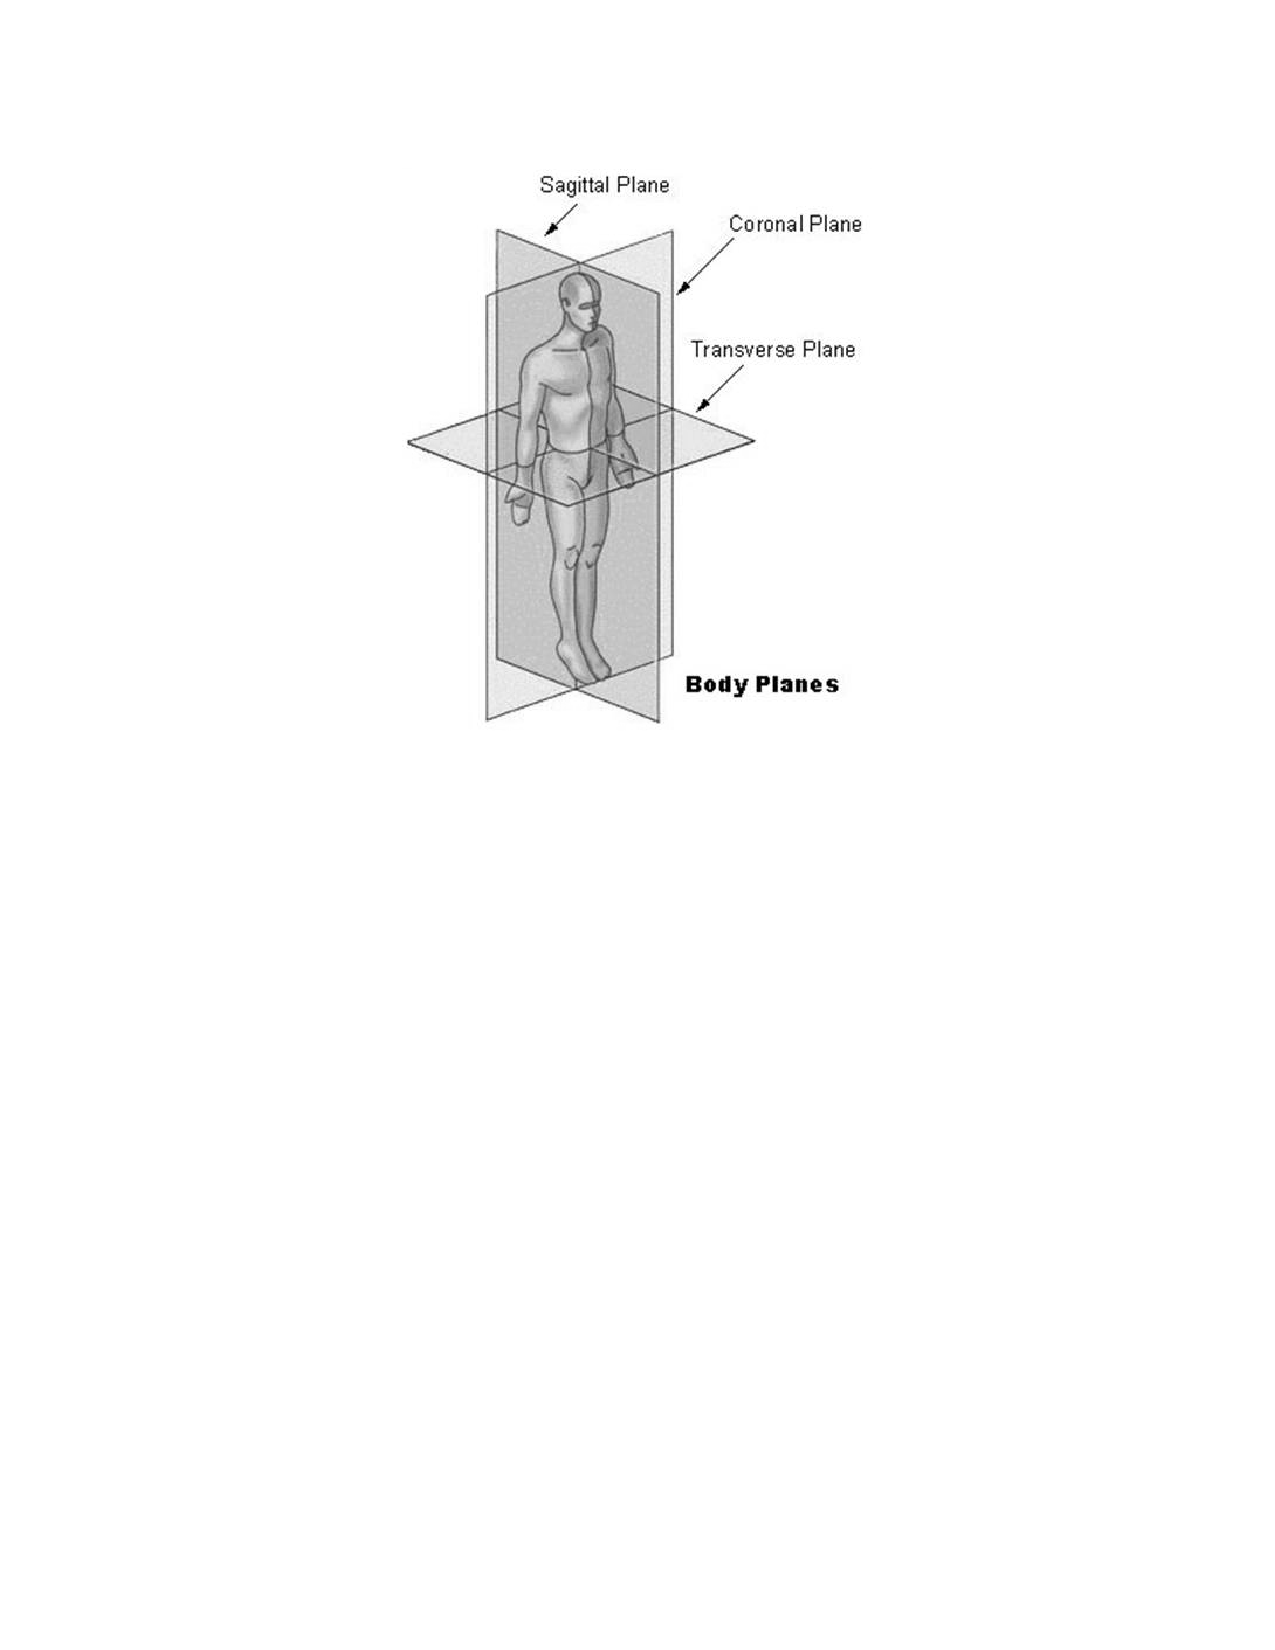
\includegraphics[height=4cm]{bodyplanes}
        \end{figure}
      \end{column}
      \begin{column}{0.6\textwidth}
        \begin{figure}
          \centering
          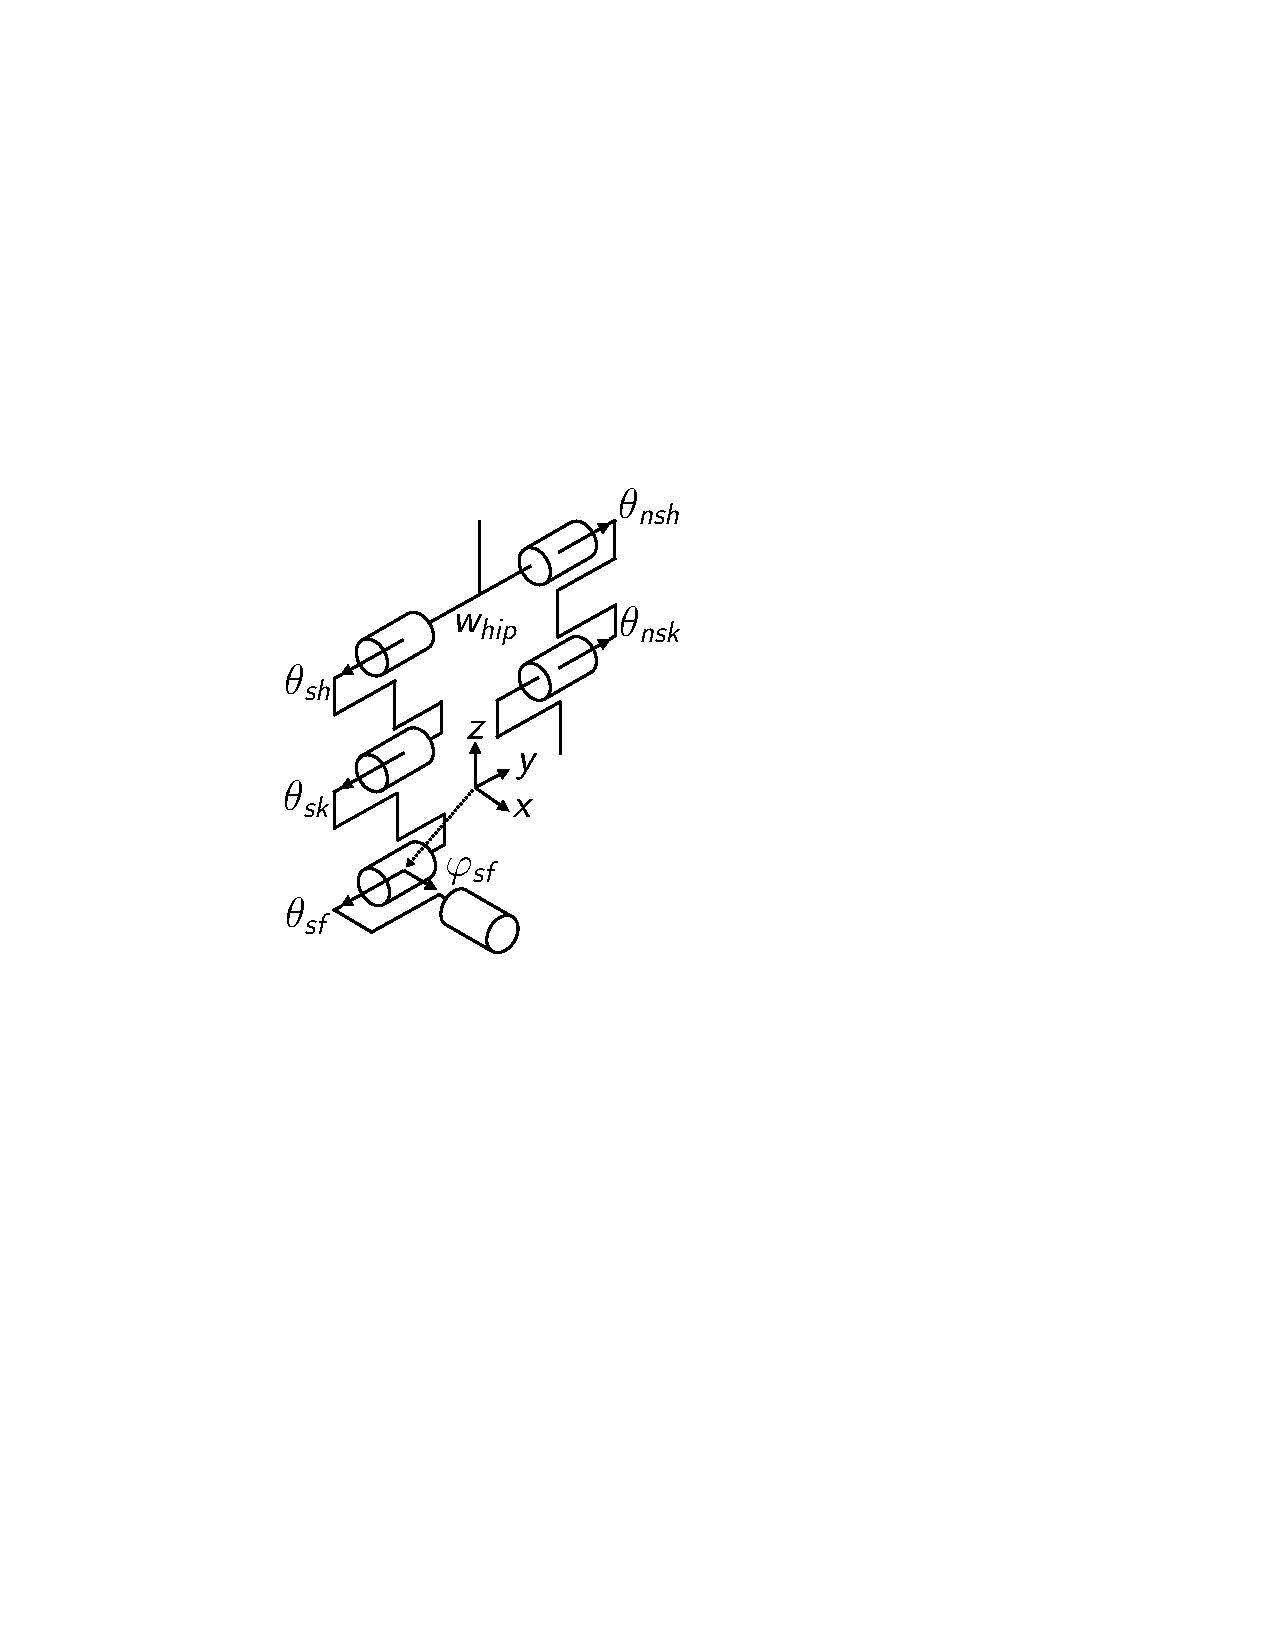
\includegraphics[height=3cm]{robot_angles_3d} \qquad
          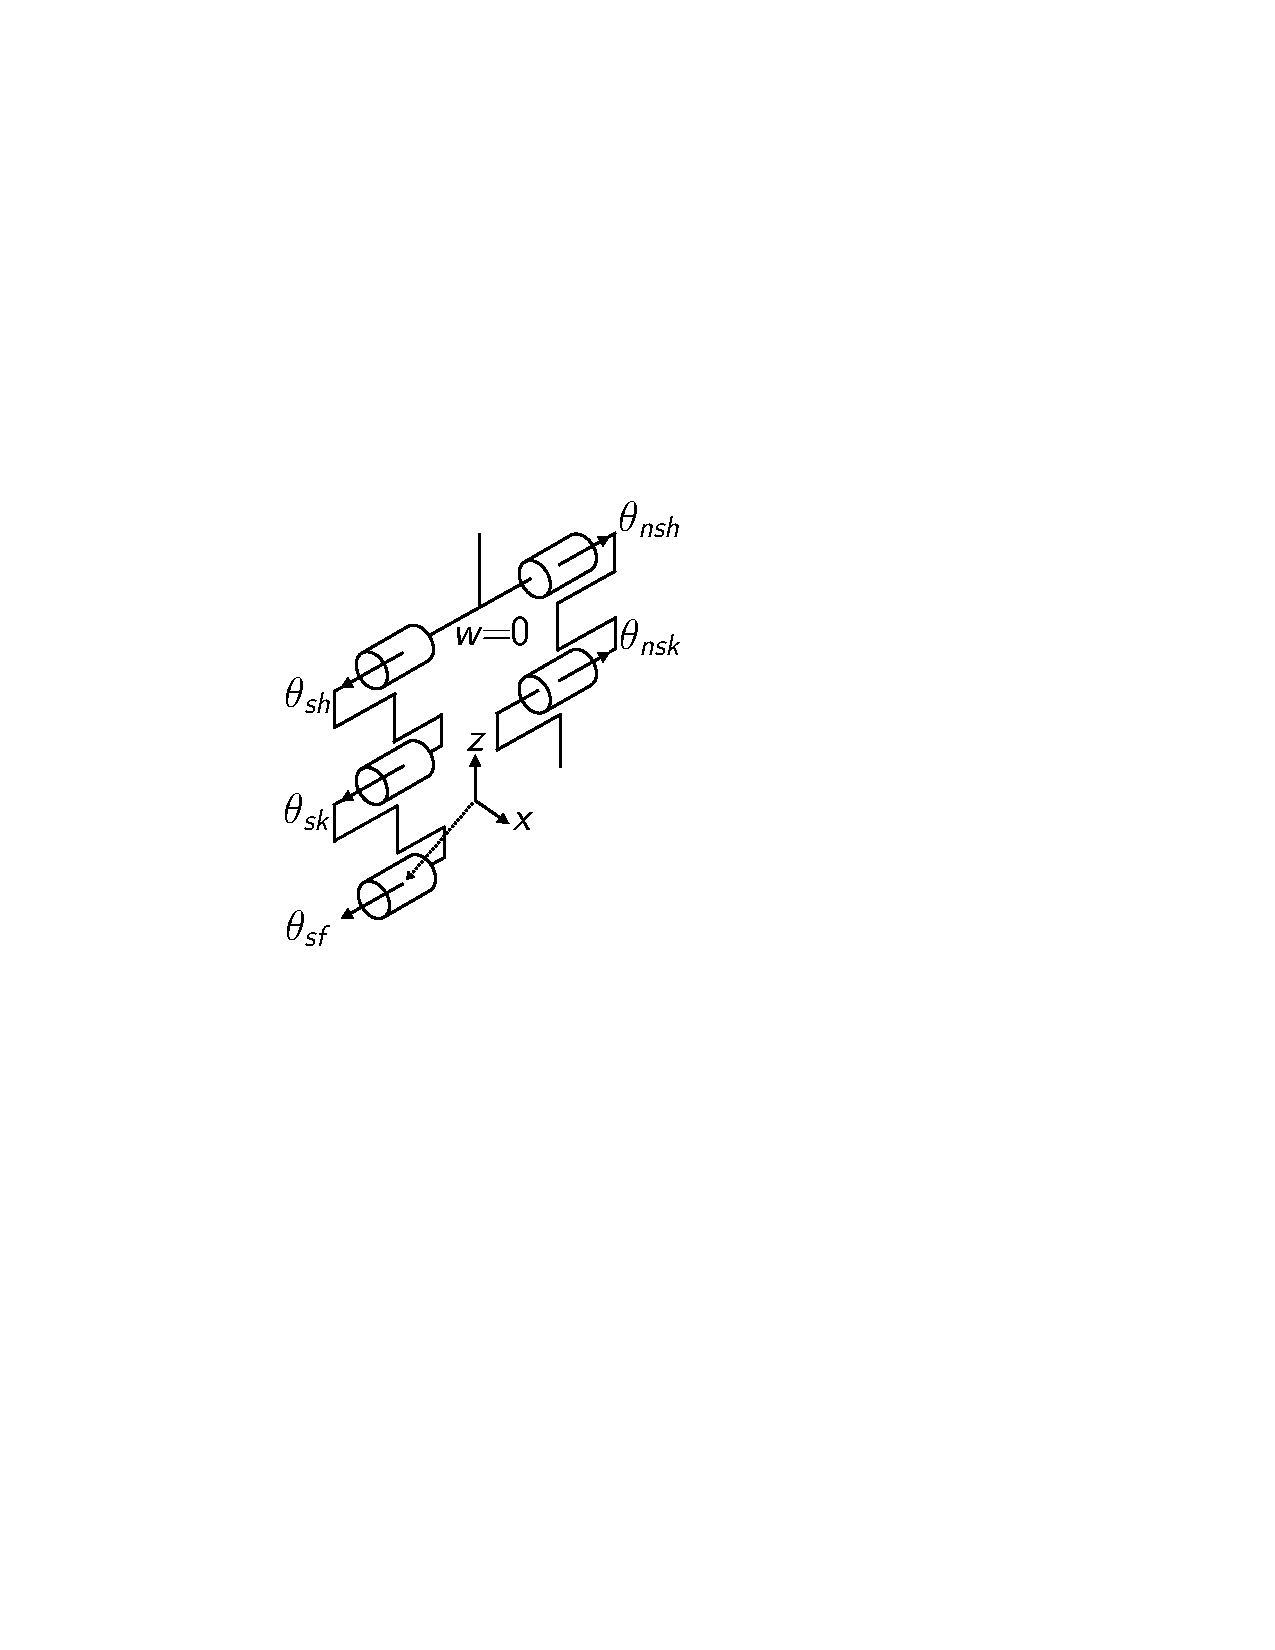
\includegraphics[height=3cm]{robot_angles_2d}
          \caption{Sagittal restriction of of 3D biped leads to a reduced model.}
        \end{figure}
      \end{column}
    \end{columns}
  }

  \only<2> {
    {\scriptsize  \textcolor{gray}{
        \begin{diagram}[width=5em,height=5em]
          \textcolor{black}{\fbox{$\begin{array}{c}$Hipped 3D Biped$\end{array}$}} &
          \rTo^{1^{\mathsf{st}} \:\: \mathsf{Reduction}}_{\mathsf{Control} \:\: \mathsf{Law}} &
          \fbox{$\begin{array}{c}$3D Biped$\\$with shaped$\\$energy$\end{array}$} &
          \rTo^{2^{\mathsf{nd}} \:\: \mathsf{Reduction}}_{\mathsf{Control} \:\: \mathsf{Law}} &
          \fbox{$\begin{array}{c}$3D Biped$\\$walking stably$\end{array}$}\\
          \dDashto^{\textcolor{black}{\mathsf{Sagittal}}}_{\textcolor{black}{\mathsf{Restriction}}} &&
          \uTo \dTo_{\begin{array}{c}$Reduction$\end{array}}&&\\
          \textcolor{black}{\fbox{$\begin{array}{c}$2D Biped$\end{array}$}} &
          \rTo^{\textcolor{black}{\mathsf{Sagittal}}}_{\textcolor{black}{\mathsf{Control} \:\: \mathsf{Law}}} &
          \textcolor{black}{\fbox{$\begin{array}{c}$2D Biped$\\$walking stably$\end{array}$}} && \\
    \end{diagram}}}
  }

  \only<3> {
    \begin{itemize}
    \item  The Lagrangian of the 3D biped has the general form:
      \begin{eqnarray}
        \label{eq:submats}
        \lefteqn{\Lfd(\cq{},\cdq{}) = -\Vu \ + }\\
        \nonumber
        &&\frac{1}{2}
        \left(\begin{array}{c c}
          \dot{\theta}^T & \dot{\varphi}
        \end{array}\right)
        \underbrace{\left(\begin{array}{c c}
            \Mth & \Mphitheta^T(\theta,\varphi)\\
            \Mphitheta(\theta,\varphi) & \Mphi(\theta,\varphi)
          \end{array}\right)}_{\mMu}
        \left(\begin{array}{c}
          \dot{\theta}\\
          \dot{\varphi}
        \end{array}\right), \nonumber
      \end{eqnarray}
      \vspace{-5mm}

    \item The Lagrangian of the sagittal restriction is given by:
      \begin{align*}
        \Lrd(\theta,\dot{\theta}) = \frac{1}{2} \dot{\theta}^T \Mth \dot{\theta} - \left.\Vu\right\vert_{\varphi=0},
      \end{align*}

    \end{itemize}
  }

  \only<4> {
    \vspace{-.1cm}
    \begin{itemize}

    \item The Lagrangian of the sagittal restriction is given by:
      \begin{align*}
        \Lrd(\theta,\dot{\theta}) = \frac{1}{2} \dot{\theta}^T \Mth \dot{\theta} - \left.\Vu\right\vert_{\varphi=0},
      \end{align*}

    \item This yields a control system: $(\fr,\gr)$.

    \item \alert{Assume} there exists a control law, $\usagarg$, that results in stable 2D waking for the dynamical system:
      \begin{align*}
        \flt = \fr(\theta, \dot{\theta}) + \gr(\theta) \usagarg.
      \end{align*}

    \end{itemize}
  }

  %\only<5> {
  %  \begin{figure}
  %    \centering
  %    \movie[width=0.6\textwidth,externalviewer]{
  %    \includegraphics[width=0.6\textwidth]{2dwalkinggait.pdf}}{Movies/2d-movie.avi}\\
  %    \includegraphics[height=0.3\textheight]{pp-2d-legs.pdf}
  %    \includegraphics[height=0.3\textheight]{pp-2d-feet.pdf}
  %  \end{figure}
  %}
  %
}

\frame[t] {
  \frametitle{$1^{\mathsf{st}}$ Reduction Control Law: Lagrangian Shaping Controller}

  Shape the total energy of the 3D biped so that functional Routhian reduction can be applied and the reduced system is exactly the 2D system obtained from the first control law.

  {\scriptsize \textcolor{gray}{
      \begin{diagram}[width=5em,height=5em]
        \textcolor{black}{\fbox{$\begin{array}{c}$Hipped 3D Biped$ \end{array}$}} &
        \rTo^{\textcolor{black}{1^{\mathsf{st}} \:\: \mathsf{Reduction}}}_{\textcolor{black}{\mathsf{Control} \:\: \mathsf{Law}}} &
        \textcolor{black}{\fbox{$\begin{array}{c}$3D Biped$\\$with shaped$\\$energy$\end{array}$}} &
        \rTo^{2^{\mathsf{nd}} \:\: \mathsf{Reduction}}_{\mathsf{Control} \:\: \mathsf{Law}} &
        \fbox{$\begin{array}{c}$3D Biped$\\$walking stably$\end{array}$}\\
        \dDashto^{\textcolor{black}{\mathsf{Sagittal}}}_{\textcolor{black}{\mathsf{Restriction}}} &&
        \uTo \dTo_{\textcolor{black}{\begin{array}{c}$Reduction$\end{array}}}&&\\
        \textcolor{black}{\fbox{$\begin{array}{c}$2D Biped$\end{array}$}} &
        \rTo^{\textcolor{black}{\mathsf{Sagittal}}}_{\textcolor{black}{\mathsf{Control} \:\: \mathsf{Law}}} &
        \textcolor{black}{\fbox{$\begin{array}{c}$2D Biped$\\$walking stably$\end{array}$}} &&
      \end{diagram}
  }}
}


\frame[t] {
  \frametitle{$2^{\mathsf{nd}}$ Reduction Control Law: Zero Dynamics Controller}

  Use feedback linearization to stabilize to the surface of initial conditions for which the decoupling promised by functional Routhian Reduction is valid.

  {\scriptsize  \textcolor{gray}{
      \begin{diagram}[width=5em,height=5em]
        \textcolor{black}{\fbox{$\begin{array}{c}$Hipped 3D Biped$\end{array}$}} &
        \rTo^{\textcolor{black}{1^{\mathsf{st}} \:\: \mathsf{Reduction}}}_{\textcolor{black}{\mathsf{Control} \:\: \mathsf{Law}}} &
        \textcolor{black}{\fbox{$\begin{array}{c}$3D Biped$\\$with shaped$\\$energy$\end{array}$}} &
        \rTo^{\textcolor{black}{2^{\mathsf{nd}} \:\: \mathsf{Reduction}}}_{\textcolor{black}{\mathsf{Control} \:\: \mathsf{Law}}} &
        \textcolor{black}{\fbox{$\begin{array}{c}$3D Biped$\\$walking stably$\end{array}$}}\\
        \dDashto^{\textcolor{black}{\mathsf{Sagittal}}}_{\textcolor{black}{\mathsf{Restriction}}} &&
        \uTo \dTo_{\textcolor{black}{\begin{array}{c}$Reduction$\end{array}}}&& \\
        \textcolor{black}{\fbox{$\begin{array}{c}$2D Biped$\end{array}$}} &
        \rTo^{\textcolor{black}{\mathsf{Sagittal}}}_{\textcolor{black}{\mathsf{Control} \:\: \mathsf{Law}}} &
        \textcolor{black}{\fbox{$\begin{array}{c}$2D Biped$\\$walking stably$\end{array}$}}&&
      \end{diagram}
  }}
}

%\section{Human-Inspired Control}
\showtoc

\subsection{Human-Inspired Control Framework}
\frame{
  \frametitle{Human Data Experiment}
  \begin{columns}
    \begin{column}{0.65\textwidth}
      \begin{figure}
        \centering
        \vspace{-1cm}
        \caption{Experimental setup showing sensor placement for human data acquisition}
        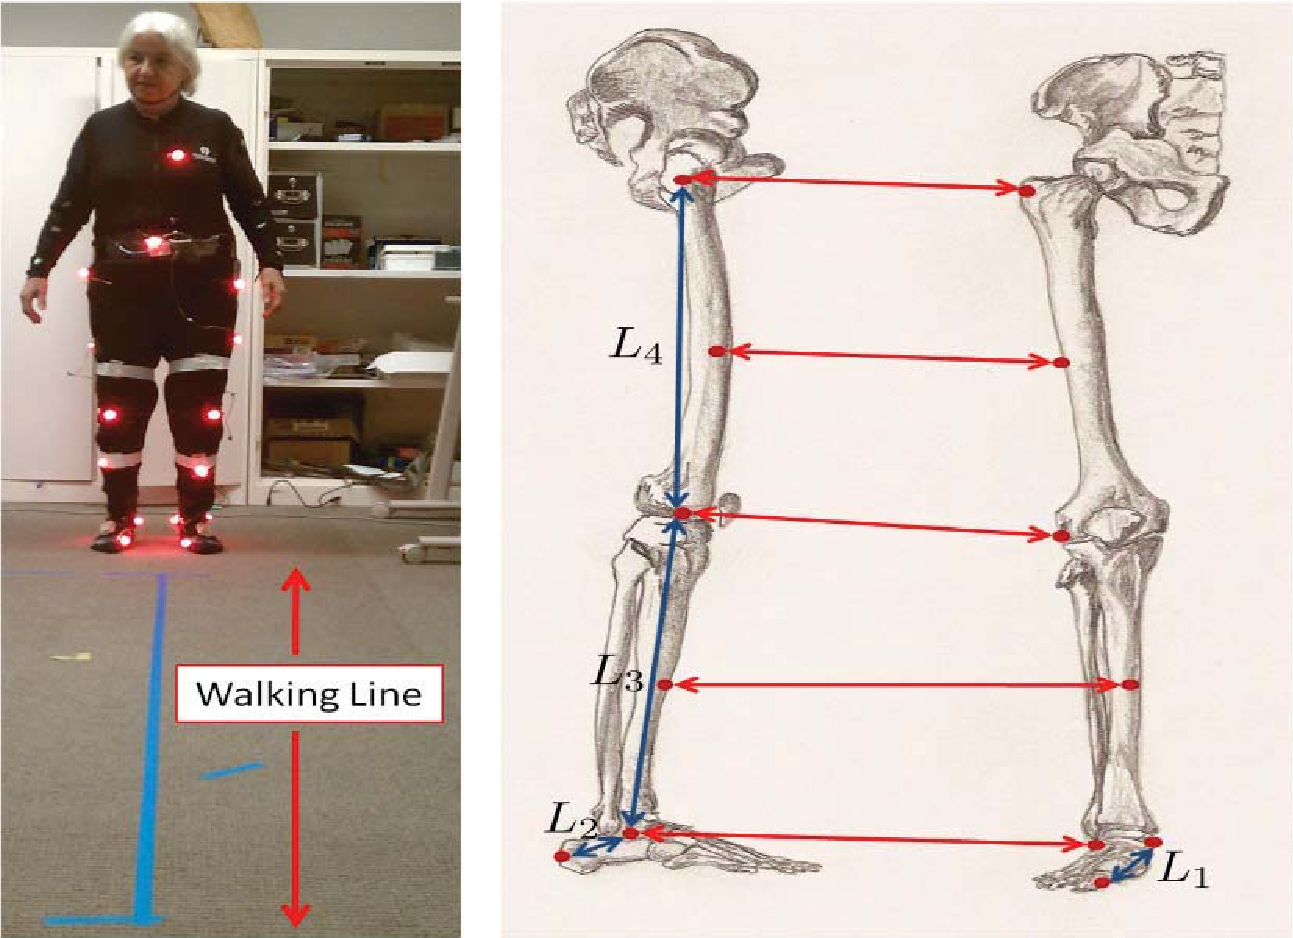
\includegraphics[width=1.0\columnwidth]{labeled_diagram}
      \end{figure}
    \end{column}
    \begin{column}{0.35\textwidth}
      \begin{figure} \centering
        \vspace{-1cm}
        \caption{Human outputs}
        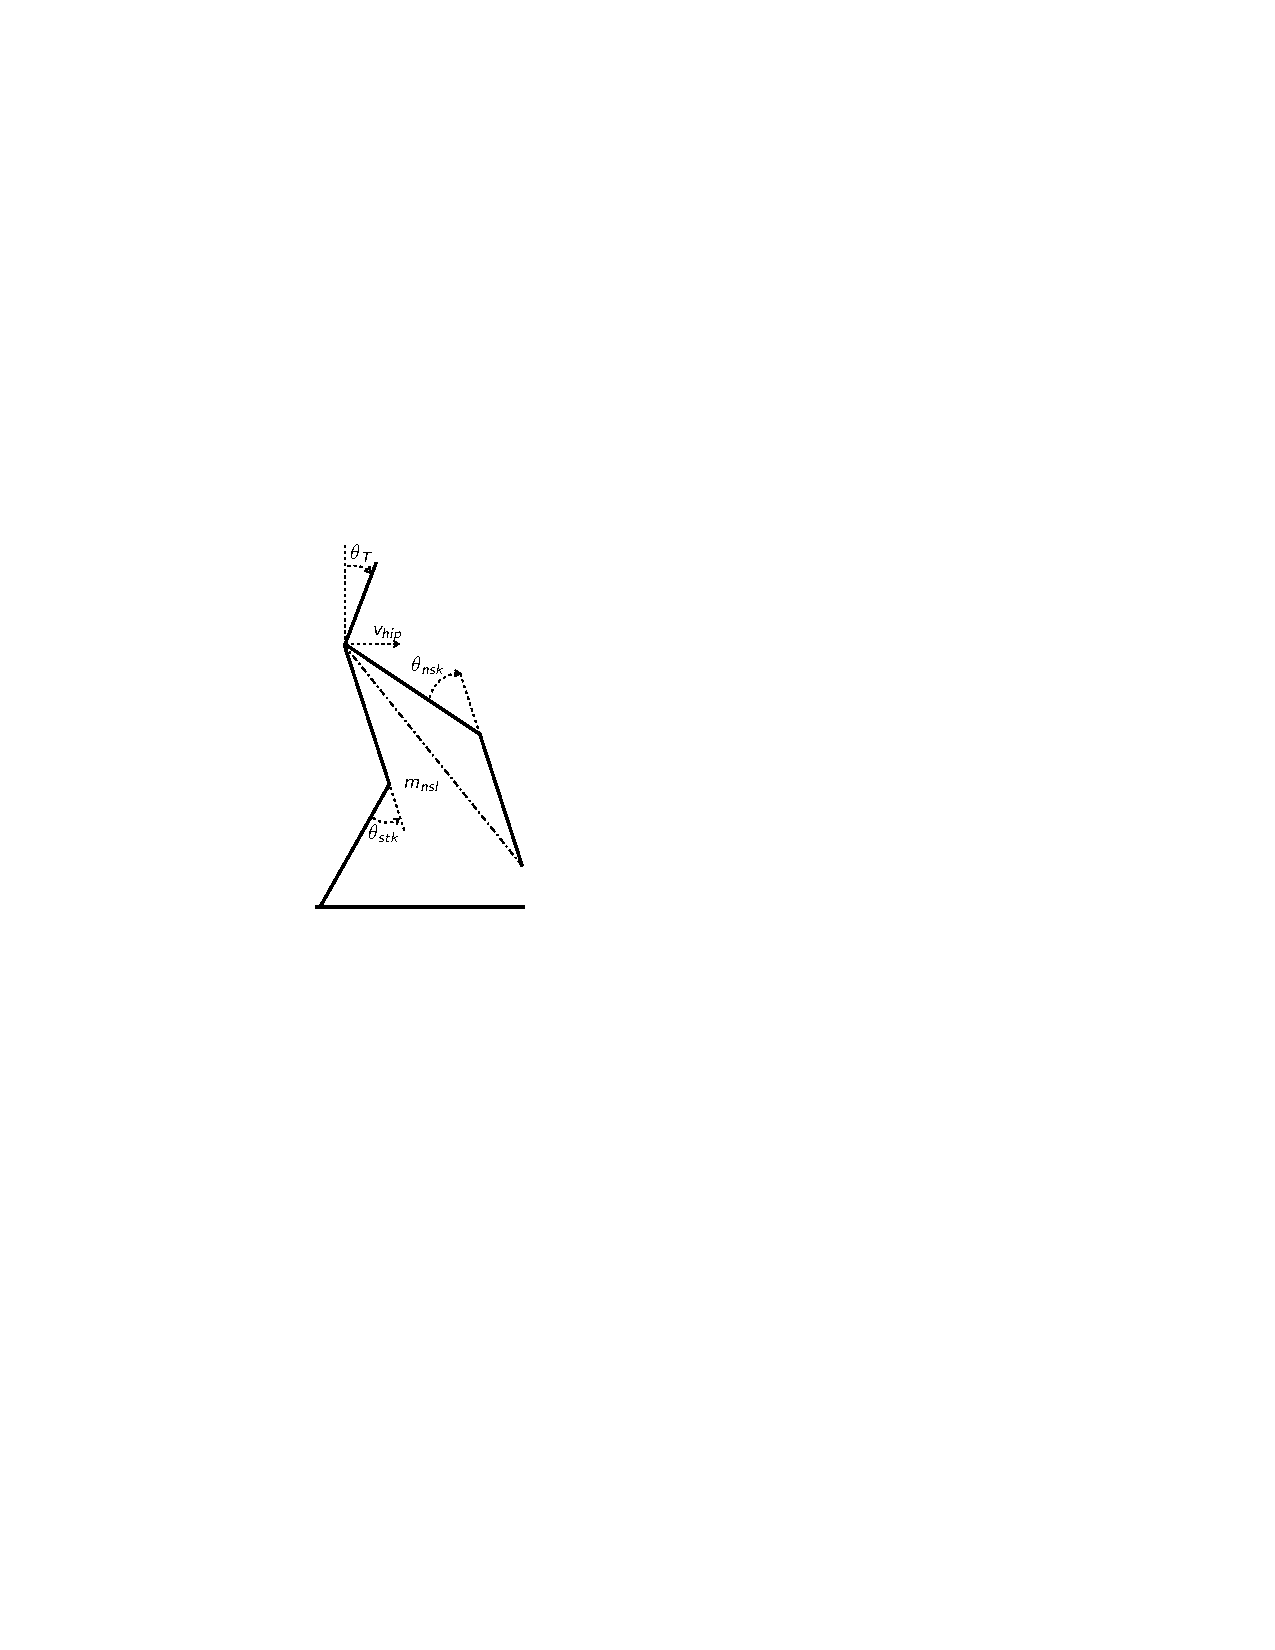
\includegraphics[width=0.8\columnwidth]{pointfoot_robot_const}
      \end{figure}
    \end{column}
  \end{columns}
}

\frame[t]{
  \frametitle{Canonical Walking Functions}
  The following function, termed the \blue{canonical walking function}, fits human kinematics data quite accurately:
  \begin{align}
    \nonumber
    y(t) &= e^{-\zeta \omega_{n} t} (c_{1} \cos (\omega_{d} t) + c_{2} \sin (\omega_{d} t)) + \hat{g}\\
    \tag{CWF}
    \label{eq:cwf}
    y^{H}(t, A)&= e^{-a_{3} t} (a_{1} \cos (a_{2} t) + a_{4} \sin (a_{2} t)) + a_{5}
  \end{align}
  where,
  \begin{itemize}
  \item
    $\zeta$ is the damping ratio,
  \item
    $\omega_{n}$, $\omega_{d}$ are the natural and damped natural frequencies, resp.,
  \item
    $c_{1}$ and $c_{2}$ are initial conditions,
  \item
    and $\hat{g}$ is from a particular solution for constant forcing.
  \end{itemize}
  Parameterize time using hip position:
  \begin{align*}
    \tau(\theta) := \frac{p_\mathit{hip}^{x}(\theta) - p_\mathit{hip}^{x}(\theta^{-})}{v_\mathit{hip}}
  \end{align*}
}

\begin{frame}[t]
  \frametitle{Example: 5-Link Biped}
  \begin{columns}
    \column{1.5in}
    Dynamic Model:
    \begin{align*}
      M(q) \ddot q + H(q, \dot q) = B(q) u
    \end{align*}
    \column{1.5in}
    \begin{figure}
      \centering
      \def\svgwidth{1.0\columnwidth}
      \input{../figs/cg2d-5link-model.eps_latex}
      \vspace{-2em}
      \caption{5-link biped configuration.}
    \end{figure}
  \end{columns}
\end{frame}

\frame{
  \frametitle{Selecting Human Outputs}
  The following human kinematics outputs are viable:
  \begin{enumerate}
    {
    \item[\HF{1}:] $\Oa$, \blue{forward hip velocity}, i.e., the velocity of the $x$-position of the hip,
    \item[\HF{2}:] $\Ob$, \blue{swing leg slope}, i.e., the tangent of the angle between the $z$-axis and the projection of the line connecting the swing ankle and hip,
    \item[\HF{3}:] $\Oc$, \blue{stance knee relative angle},
    \item[\HF{4}:] $\Od$, \blue{swing knee relative angle},
    \item[\HF{5}:] $\Oe$, \blue{vertical torso angle}, the angle of the torso measured with respect to the vertical axis of the world frame.
    }
  \end{enumerate}

  \vspace{1mm}
  For convenience, define the actual and desired outputs:
  \vspace{-1mm}
  \begin{align*}
    y_{1}^{a} = \Oa, \ y_{2}^{a} = \Ob, \ y_{3}^{a} = \Oc, \ y_{4}^{a} = \Od, \ y_{5}^{a} = \Oe,
  \end{align*}
  \vspace{-8mm}
  \begin{align*}
    y_{1}^{d} = y^{H}(\tau(\theta), A_1), \ \ldots, \ y_{5}^{d} = y^{H}(\tau(\theta), A_5)
  \end{align*}
}

\frame{
  \frametitle{Human-Inspired Optimization}
  The form of \eqref{eq:cwf} allows it to encode certain outputs:
  \vspace{-4mm}
  \begin{figure}
    \centering
    \caption{Canonical walking functions with parameters from \eqref{eq:opt}}
    \vspace{-2mm}
    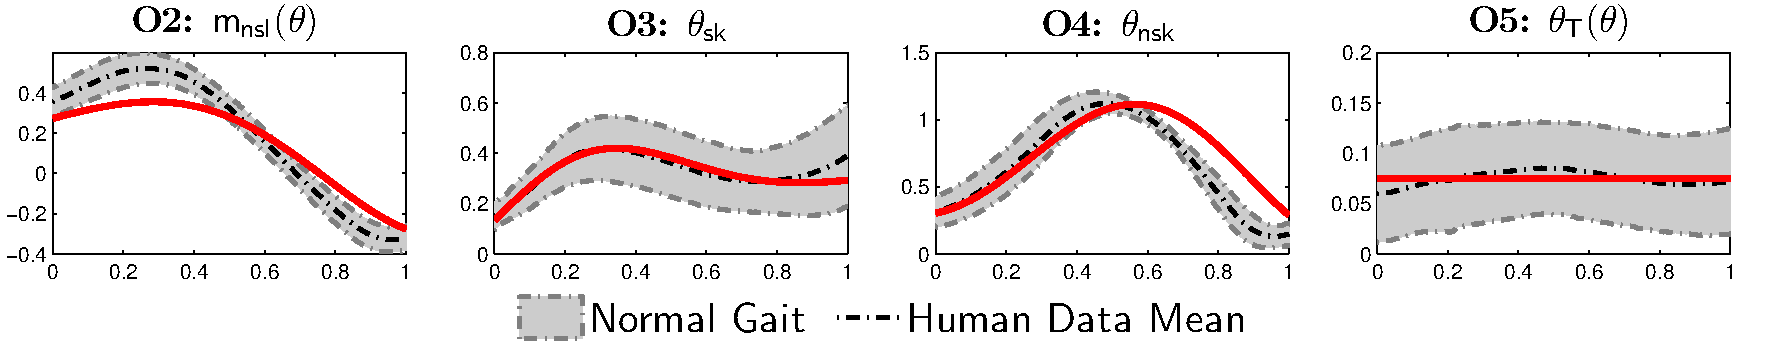
\includegraphics[width=1.0\textwidth]{human_function_fits}
    \vspace{-2mm}
  \end{figure}
  These outputs can be used to construct a \blue{partial hybrid zero dynamics} parameterized by matrix $A$ where outputs \textcolor{blue}{\HF{2}}--\textcolor{blue}{\HF{5}} of the robot are equal to the desired outputs for all time. The optimal parameters $A^*$ are found by solving
  \begin{align}
    \label{eq:opt}
    \tag{$\mathcal{O}$}
    A^{*} = \underset{A \in \R^{5 \times 5}}{\operatorname{argmin}} &  \:\: \mathrm{Cost}_{\mathrm{HD}}(A)  \\[-1mm]
    \nonumber
    \mathrm{s.t.} \quad & \ResetMapReduced(\GuardReduced \cap \HZD_{A}) \subset \PHZD_{A}
  \end{align}
}

\begin{frame}[t]
  \frametitle{Tracking the Partial Hybrid Zero Dynamics}
  Tracking can be accomplished with a variety of control schemes. PD control is interesting due to its model-independent nature:
  \begin{align*}
    \mathcal{K}_{2D}(\theta, \dot{\theta}) \! = \! k_p \left(\!\!
    \begin{array}{c}
      0\\
      y_{d,2} - y_{a,2}\\
      y_{d,3} - y_{a,3}\\
      y_{d,4} - y_{a,4}\\
      y_{d,5} - y_{a,5}
    \end{array}\!\!\right)  + 
    \blkdiag (k_p, k_d I_4)\left(\!\!
    \begin{array}{c}
      y_{d,1} - y_{a,1}\\
      \dot{y}_{d,2} - \dot{y}_{a,2}\\
      \dot{y}_{d,3} - \dot{y}_{a,3}\\
      \dot{y}_{d,4} - \dot{y}_{a,4}\\
      \dot{y}_{d,5} - \dot{y}_{a,5}
    \end{array}\!\!\right)
  \end{align*}

  This control law will result in walking in simulation (and in experiment in other works) and will satisfy assumptions made by functional Routhian reduction (introduced later).
\end{frame}

\begin{frame}[t]
  \frametitle{Procedure Summary}
  \begin{figure}
    \includemedia[
      width=0.8\columnwidth,
      height=0.45\columnwidth,
      addresource=human_experiment.mp4,
      activate=pageopen,
      flashvars={source=human_experiment.mp4&loop=true&autoPlay=true}
    ]{}{VPlayer9.swf}
    \caption{Human-inspired control produces robotic gaits from human data.}
  \end{figure}
\end{frame}

\begin{frame}[t]
  \frametitle{3D Simulation Results}
  \only<1>{
    \begin{figure}
      \centering
      \caption{Walking gait for 3D model with $v_\mathit{hip} = .6$ m/s}
      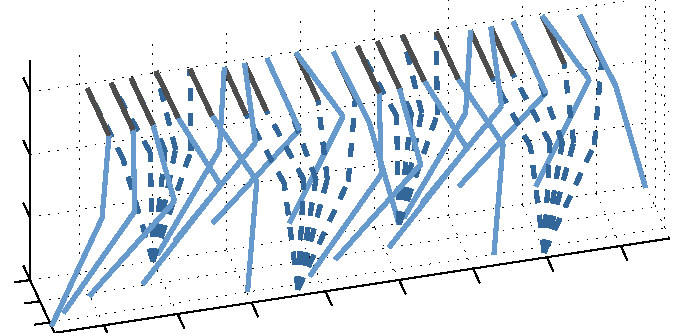
\includegraphics[width=.9\textwidth]{hic_frr_tiles_3d}
    \end{figure}
  }
  \only<2>{
    \begin{figure}
      \centering
      \caption{Phase portraits, human outputs, and actuator torques}
      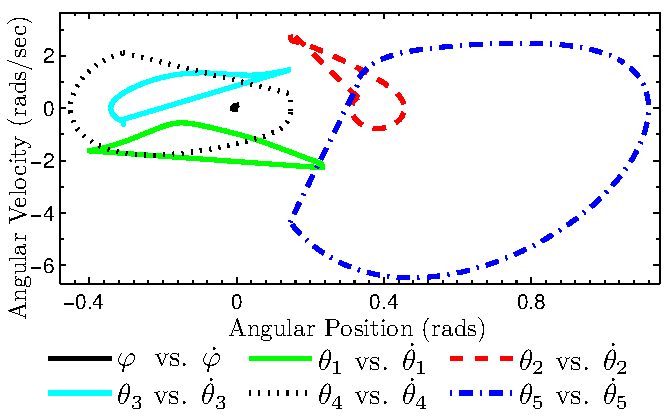
\includegraphics[width=.4\textwidth]{hic_frr_pp_3d_theta}\quad
      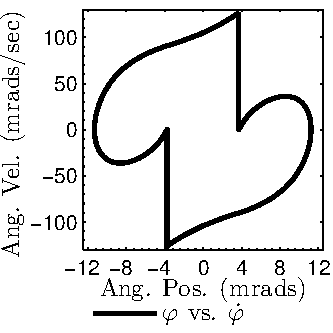
\includegraphics[width=.25\textwidth]{hic_frr_pp_3d_phi}\\[.3em]
      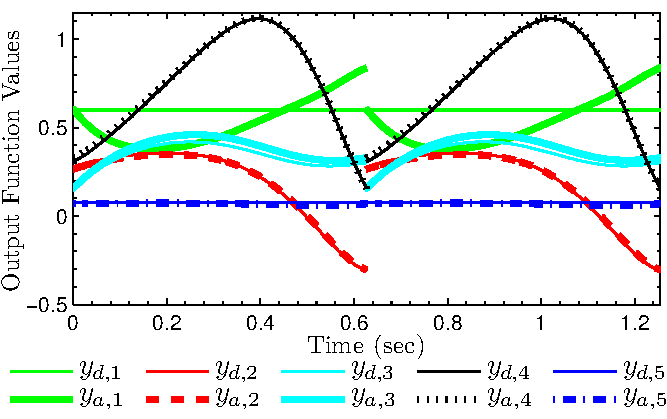
\includegraphics[width=.4\textwidth]{hic_frr_outputs_3d}\quad
      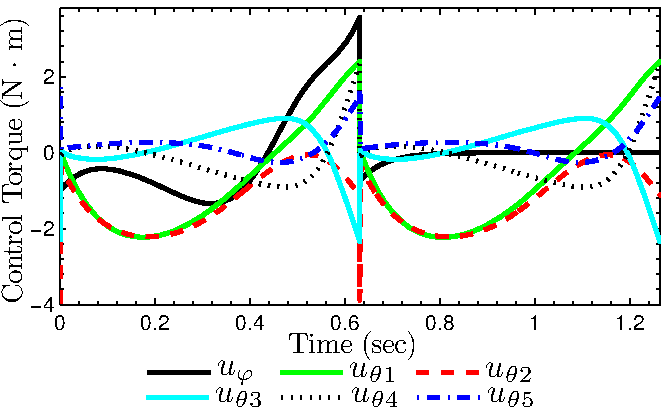
\includegraphics[width=.4\textwidth]{hic_frr_torques_3d}
    \end{figure}
  }
\end{frame}

\begin{frame}[t]
  \frametitle{3D Experiment Results}
  \begin{figure}
    \centering
    \caption{Experimental validation of HIC/FRR scheme}
    \only<1>{
      \includegraphics[height=2cm]{nao_tiles}\\[.3em]
      \includegraphics[height=3.25cm]{exp_angles}
    }
    \only<2>{
      \includemedia[
        %width=1.0\columnwidth,
        %height=0.5625\columnwidth,
        width=1.0\columnwidth,
        height=0.5\columnwidth,
        addresource=nao_reduction.mp4,
        activate=pageopen,
        flashvars={source=nao_reduction.mp4&loop=true&autoPlay=true}
      ]{}{VPlayer9.swf}
    }
  \end{figure}
\end{frame}

\begin{frame}[t]
  \frametitle{Combining ES and HIC}
  \only<1>{
    \begin{figure}
      \centering
      \includegraphics[width=1.0\columnwidth]{energy_conserved_5link}
      \caption{Demonstration of Energy Shaping and Human-Inspired Control.}
    \end{figure}
  }

  \only<2>{
    \begin{figure}
      \centering
      \includemedia[
        %width=1.0\columnwidth,
        %height=0.5625\columnwidth,
        width=1.0\columnwidth,
        height=0.5\columnwidth,
        addresource=5link_es.mp4,
        activate=pageopen,
        flashvars={source=5link_es.mp4&loop=true&autoPlay=true}
      ]{}{VPlayer9.swf}
      \caption{Energy shaping to stabilize to a gait from distant initial condition.}
    \end{figure}
  }
\end{frame}


%\section{Conclusions}
\showtoc

\subsection{Remaining Work and Concluding Remarks}
\begin{frame}
  \frametitle{Current Results}
  \begin{itemize}
  \item 2D Compass-gait
  \item 2D 3-link
  \item 3D 3-link
  \item 2D 7-link
  \item 2D 5-link with HIC
  \end{itemize}
\end{frame}

\begin{frame}
  \frametitle{Remaining Work}
  \begin{itemize}
  \item 3D 5-link ES+HIC+FRR
  \item Formal proof of energy shaping
  \item 3D 7-link
  \item Application to SLIP model
  \end{itemize}
\end{frame}

\begin{frame}
  \frametitle{Questions}
  \Large{Questions?}
\end{frame}


\end{document}
